%%% aQGC %%%
\chapter{Interpretation with Effective Field Theory}
\label{chap:aQGC}
Given the results in chapter~\ref{chap:results} that there is no significant excess against the SM expectations, the limits on new physics contributions are evaluated in this chapter.
%\subsection{Introduction}
%The boson field self-interactions respect the $SU(2)\times U(1)_Y$ gauge invariance in the electroweak sector of the SM and serve as a very sensitive tool to search for the manifestations of physics beyond the SM.
%The VBS is one of the processes directly sensitive to the quartic-gauge coupling vertices of the SM.
%Variations of these vertices from the SM are known as anomalous quartic-gauge couplings (aQGC), and can arise from alterations of the electroweak or Higgs sector of the SM.
%The effect of such new physics introduced by aQGC can be realized using the effective field theory~\cite{degrande2013effective} and linearly parameterized by the effective Lagrangian as:
%\begin{equation*}
%  \mathcal{L}=\mathcal{L}_{sm}+\sum_{i}\frac{c_i}{\Lambda^{2}}\mathcal{L}_i+\sum_{n}\frac{f_n}{\Lambda^{4}}\mathcal{L}_n,
%\end{equation*}
%where $\mathcal{L}$ represents possible dim-6 and dim-8 operators and $c_i$ and $f_n$ are correspond their Wilson coefficients. The $\Lambda$ represents the energy scale over which the new degrees of freedom are integrated out. 
%In this note, the name of Lagrangian term that contains the given operator is denoted by its Wilson coefficient i.e. $L_{n} = \frac{f_{n}}{\Lambda^4} O_{n}$ is called as $f_{n}$.
%The odd-dimension operators violate lepton and baryon number conservation and are ignored.
%Both of dim-6 and dim-8 operators can contribute to the VBS processes through aTGC and aQGC, respectively,
%but due to the tight constraints of dim-6 operators from inclusive diboson measurements, only dim-8 operators are discussed in this note.
%The Eboli model~\cite{eboli2006p} is employed to describe the signals, which introduces twentyone new dim-8 operators satisfying the SM $SU(2)\times U(1)_Y$ symmetry. 
%These operators can be categorized by the types of the coupling; scalar types that contain just covariant derivatives of the Higgs field: $f_{S0}$, $f_{S1}$, $f_{S2}$, tensor types  that contain just field strengths: $f_{T0}$, ..., $f_{T9}$, and mixed operators that exhibit two covariant derivatives of the Higgs field and two field strengths: $f_{M0}$, ..., $f_{M7}$. 
%Table~\ref{tab:operators} shows the vertices that can be modified by the given operator. 
%The operators $f_{S0}$ and $f_{S2}$ are Hermitian conjugates, so they are treated as one single operator by setting both coefficients to be the same value.
%The semileptonic VBS is a golden channel that can test nineteen oeperators simultaneously, which has  $WW$, $WZ$, and $ZZ$ pairs in the final state.
%It is found via simulations that the tensor operators produce purely transversely polarized $W/Z$ bosons, while the scalar operators longitudinal bosons.
%In particular in the merged analysis, higher selection efficiency for the scalar operators is expected since the boosted boson tagger is optimized for the logitudinally-polarized bosons.

%\begin{table}[ht!]
%\begin{center}
%\resizebox{0.70\textwidth}{!}{
%\begin{tabular}{|c|c|c|c|c|c|c|c|c|c|}
%\hline & WWWW & WWZZ & ZZZZ & WWAZ & WWAA & ZZZA & ZZAA & ZAAA & AAAA \\
%\hline $\mathcal{L}_{S02}, \mathcal{L}_{S1}$ & $\mathrm{X}$ & $\mathrm{X}$ & $\mathrm{X}$ & %$\mathrm{O}$ & $\mathrm{O}$ & $\mathrm{O}$ & $\mathrm{O}$ & $\mathrm{O}$ & $\mathrm{O}$ \\
%\hline $\mathcal{L}_{M0}, \mathcal{L}_{M1}, \mathcal{L}_{M6}, \mathcal{L}_{M7}$ & $\mathrm{X}$ & %$\mathrm{X}$ & $\mathrm{X}$ & $\mathrm{X}$ & $\mathrm{X}$ & $\mathrm{X}$ & $\mathrm{X}$ & %$\mathrm{O}$ & $\mathrm{O}$ \\
%\hline $\mathcal{L}_{M2}, \mathcal{L}_{M3}, \mathcal{L}_{M4}, \mathcal{L}_{M5}$ & $\mathrm{O}$ & %$\mathrm{X}$ & $\mathrm{X}$ & $\mathrm{X}$ & $\mathrm{X}$ & $\mathrm{X}$ & $\mathrm{X}$ & %$\mathrm{O}$ & $\mathrm{O}$ \\
%\hline $\mathcal{L}_{T0}, \mathcal{L}_{T1}, \mathcal{L}_{T2}$ & $\mathrm{X}$ & $\mathrm{X}$ & %$\mathrm{X}$ & $\mathrm{X}$ & $\mathrm{X}$ & $\mathrm{X}$ & $\mathrm{X}$ & $\mathrm{X}$ & %$\mathrm{X}$ \\
%\hline $\mathcal{L}_{T5}, \mathcal{L}_{T6}, \mathcal{L}_{T7}$ & $\mathrm{O}$ & $\mathrm{X}$ & %$\mathrm{X}$ & $\mathrm{X}$ & $\mathrm{X}$ & $\mathrm{X}$ & $\mathrm{X}$ & $\mathrm{X}$ & %$\mathrm{X}$ \\
%\hline $\mathcal{L}_{T8}, \mathcal{L}_{T9}$ & $\mathrm{O}$ & $\mathrm{O}$ & $\mathrm{X}$ & $\mathrm{O}$ & $\mathrm{O}$ & $\mathrm{X}$ & $\mathrm{X}$ & $\mathrm{X}$ & $\mathrm{X}$ \\
%\hline
%\end{tabular}
%}
%\caption{Correspondences between Wilson coefficients and vertices. $\mathrm{X}$ shows the existence of the vertex with the interaction by the operator.}
%\label{tab:operators}
%\end{center}
%\end{table}

As mentioned in Section~\ref{subsec:EFT}, aQGC interpretation is done via EFT Lagrangian. 
The SM+EFT matrix element can be written as
\begin{equation}
   |A_{SM}+\frac{f_i}{\Lambda^4}A_i|^2=|A_{SM}|^2+\sum\limits_i \frac{f_i^2}{\Lambda^8}|A_{i}|^2+ \sum\limits_i 2 \frac{f_i}{\Lambda^4} \mathrm{Re}(A_{SM}^\star A_i) +\sum\limits_{i\neq j} \frac{f_i}{\Lambda^4} \frac{f_j}{\Lambda^4} \mathrm{Re}(A_i^\star A_j)
\end{equation}
where $|A_SM|^2$ is the SM matrix element, $|A_{i}|^2$ represents the pure-EFT matrix elements for the $O_{i}$ operator listed in eq~\ref{eq:OpratorFS}-\ref{eq:OpratorFT} , $2 \mathrm{Re}(A_{SM}^\star A_i)$ is its corresponding interference term with the SM, and $\mathrm{Re}(A_i^\star A_j)$ is possible interference term between EFT operators $O_{i}$ and $O_{j}$. 
Theoretically, it cannot separate the effects of Wilson coefficients $f_i$ and the scale $\Lambda^4$, so the parameter of interest in this analysis is the ratio $\frac{f_i}{\Lambda^4}$. %Sometimes it is just called as $f_i$.
The pure-EFT term is scaled by the quadrature of $\frac{f_i}{\Lambda^4}$ and the interference term by $\frac{f_{i}}{\Lambda^4}$.
They are also called as the quadratic term and the interference (linear) term, respectively.
%interference term is neglected in this analysis
In this analysis, the term with $\mathrm{Re}(A_i^\star A_j)$ is ignored for simplicity and for consistency to other previous results on aQGC search, and evaluate the contributions from each operator on a one-by-one basis.
\section{Statistical interpretation}
The aQGC signal is extracted with a profile-likelihood fit as described in section~\ref{sec:likelihood}, but replacing the signal to the aQGC sample, and the standard model EW VV+jj signal is included as background with other standard model background samples.
The POI is set as $\mu_{\mathrm{aQGC}} = \frac{f_i}{\Lambda^4}$, where signal template is defined as $\mu_{\mathrm{aQGC}}^2*$~quadratic~signal $+$ $\mu_{\mathrm{aQGC}}*$~interference~signal.
%The signal strength, $\mu$ is interpreted in terms of Wilson coefficient, $\mu$ = $\frac{f_i}{\Lambda^4}$. 
%The POI is set to include both quadratic terms and interference terms simultaneously, thereby two signal strength is parameterized as $\mu_{QUAD} = \mu_{INT}^2$.
Figure~\ref{fig:quadint} shows the quadratic and interference signal distributions of di-boson invariant mass ($m_{VV}$) in HP SR.
All $m_{VV}$ distributions for other Wilson coefficients are shown in appendix~\ref{app:aQGCresults}.  
The contribution of quadratic term and the linear term depends on the magnitude of $\mu_\mathrm{aQGC}$.
As figure~\ref{fig:largemu} shows, the contribution of the quardratic term is dominant where the $\mu_\mathrm{aQGC}$ is large, and the number of signal becomes more symmetrical. Where the $\mu_\mathrm{aQGC}$ is small, the interference term contribution is dominant, the number of signal becomes more asymmetrical and can take negative values.
\begin{figure}[ht]
    \centering
        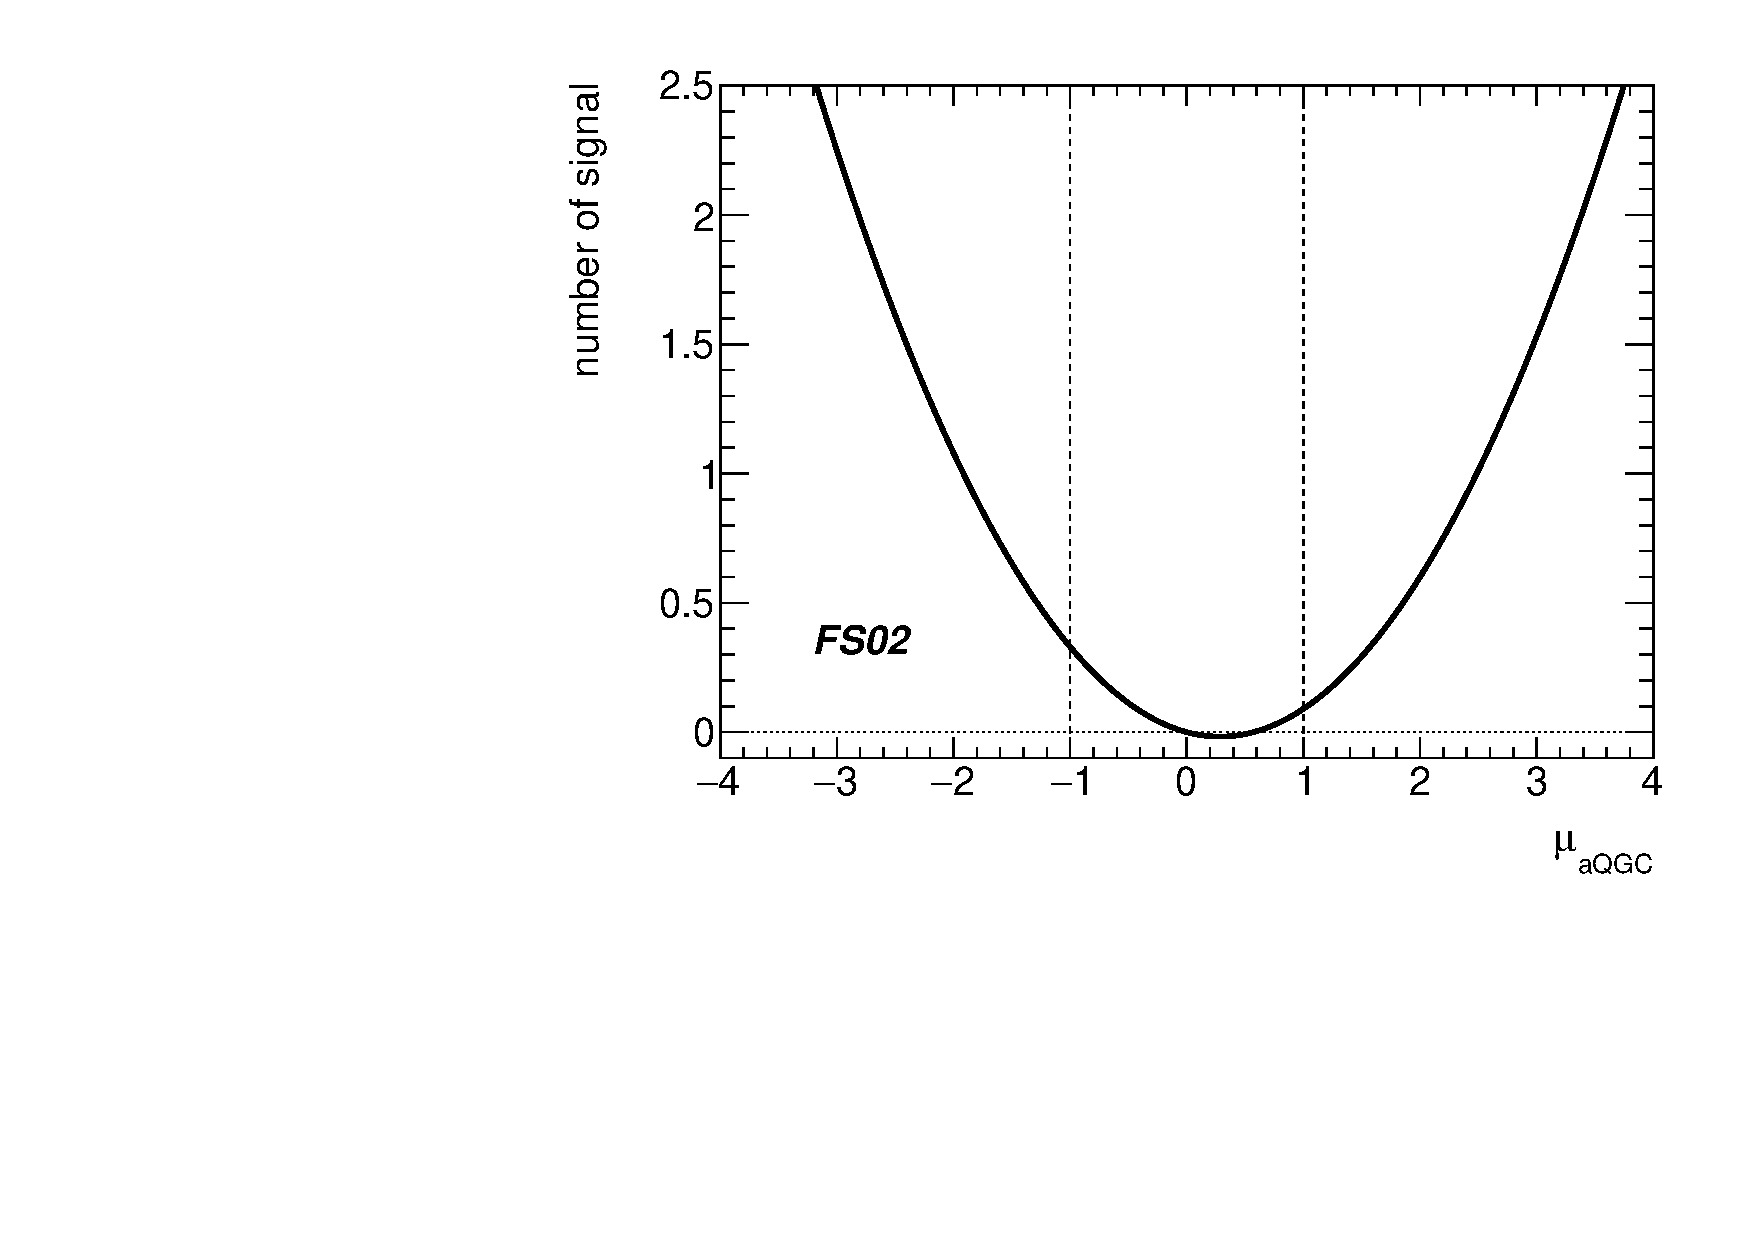
\includegraphics[width=0.50\textwidth]{figures/aQGC/largemu.pdf}
        \caption{Number of the FS02 signals with respect to the $\mu_\mathrm{aQGC}$ value. The signal is produced at $\frac{f_i}{\Lambda^4} = 1~[\mathrm{TeV}^{-4}]$. }
        \label{fig:largemu}
\end{figure}
%, the region which has the most signal constraining power in the 2-lepton channel.
\begin{figure}[ht]
    \centering
        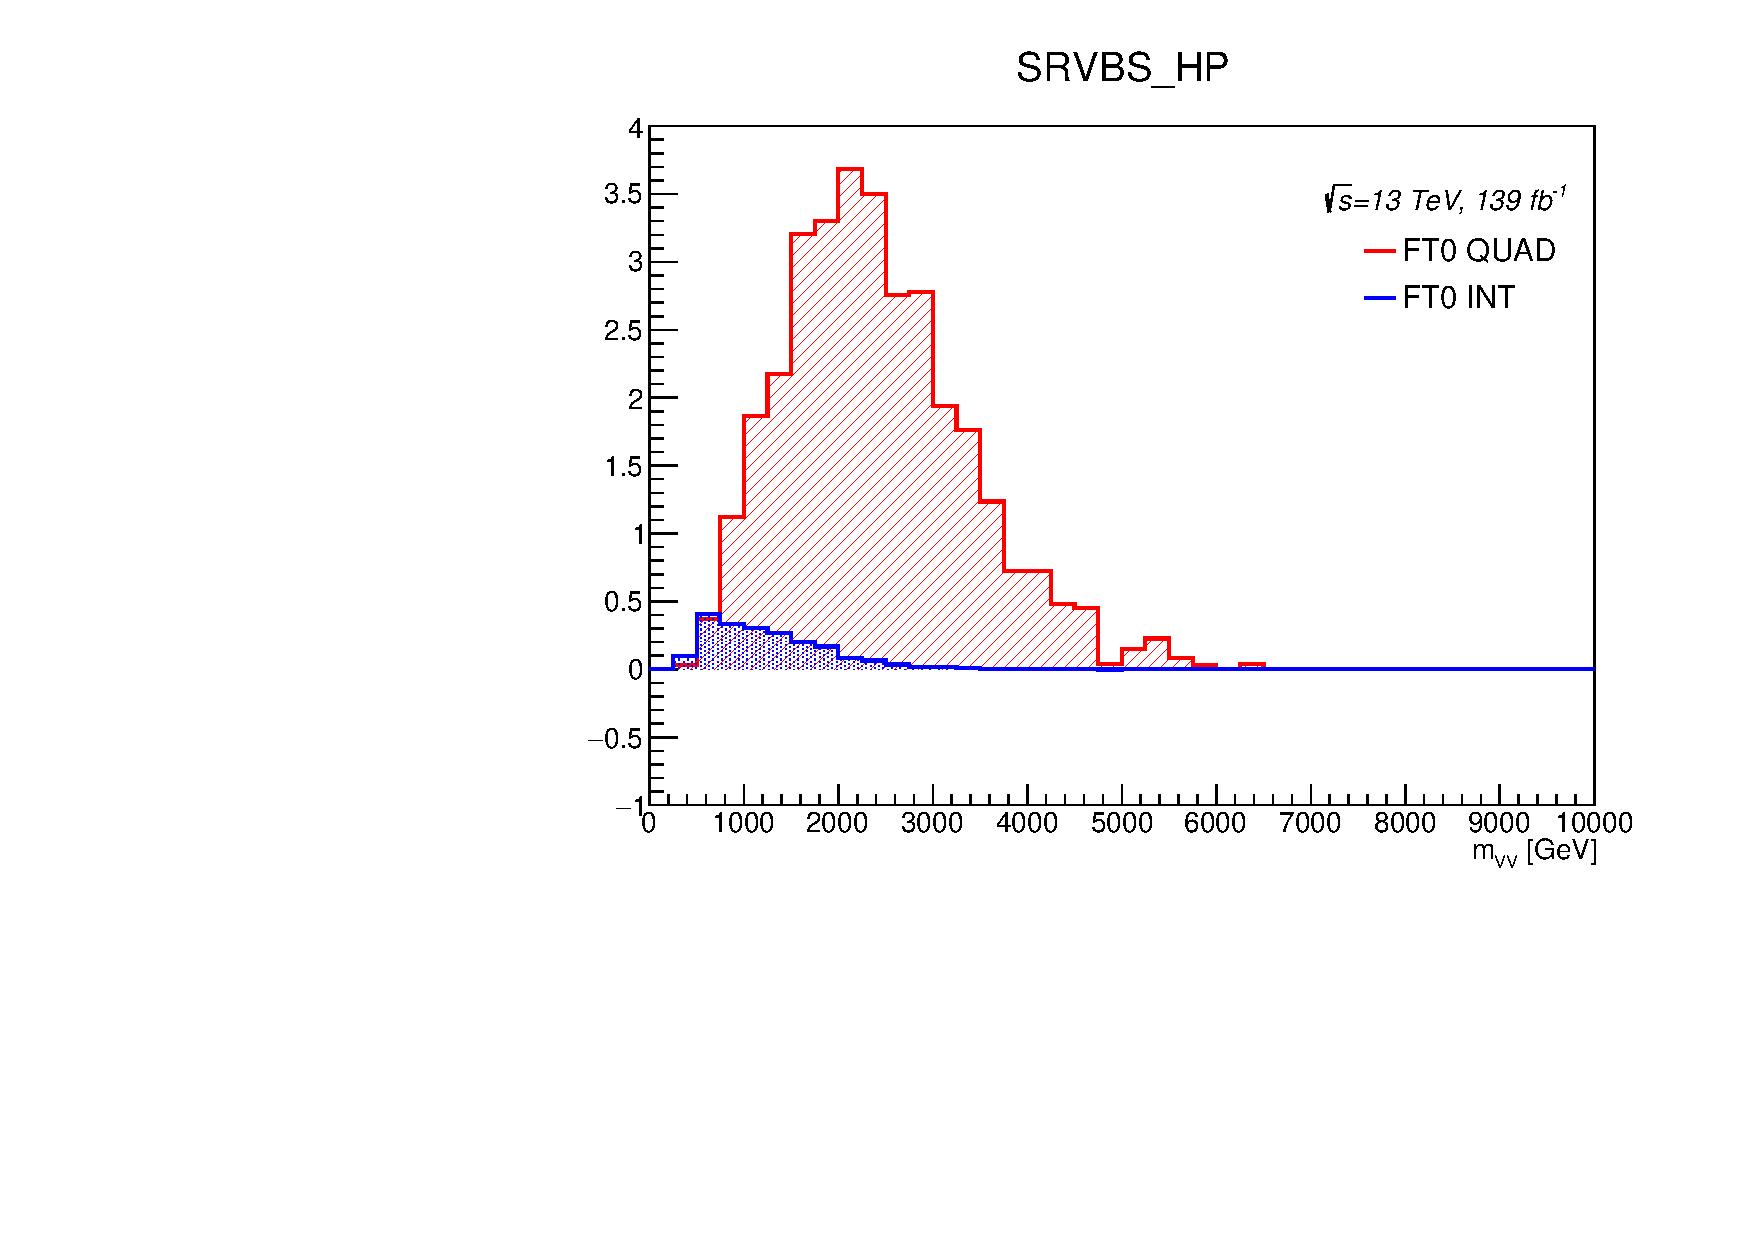
\includegraphics[width=0.45\textwidth]{figures/aQGC/FT0_0ptag1pfat0pjet_0ptv_SRVBS_HP_MllJ.pdf}
    	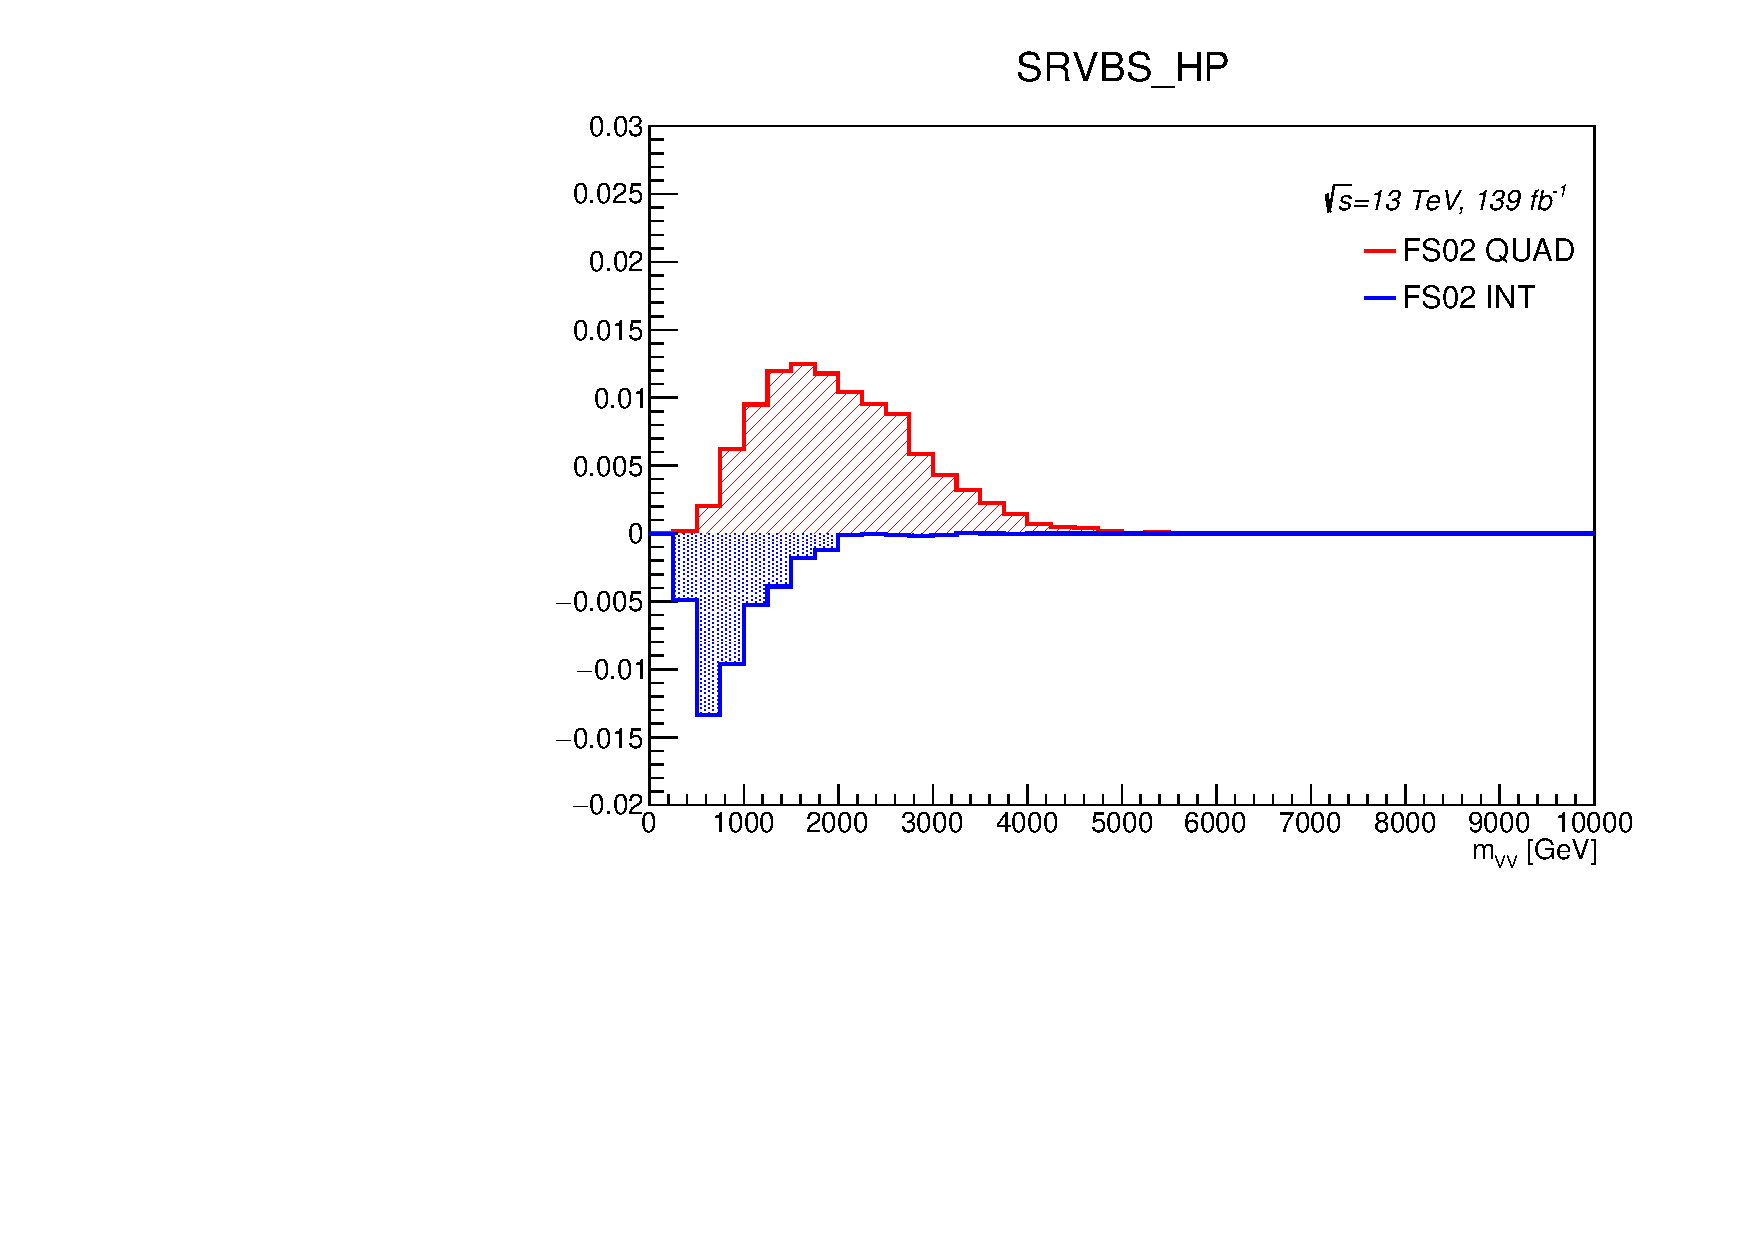
\includegraphics[width=0.45\textwidth]{figures/aQGC/FS02_0ptag1pfat0pjet_0ptv_SRVBS_HP_MllJ.pdf}
        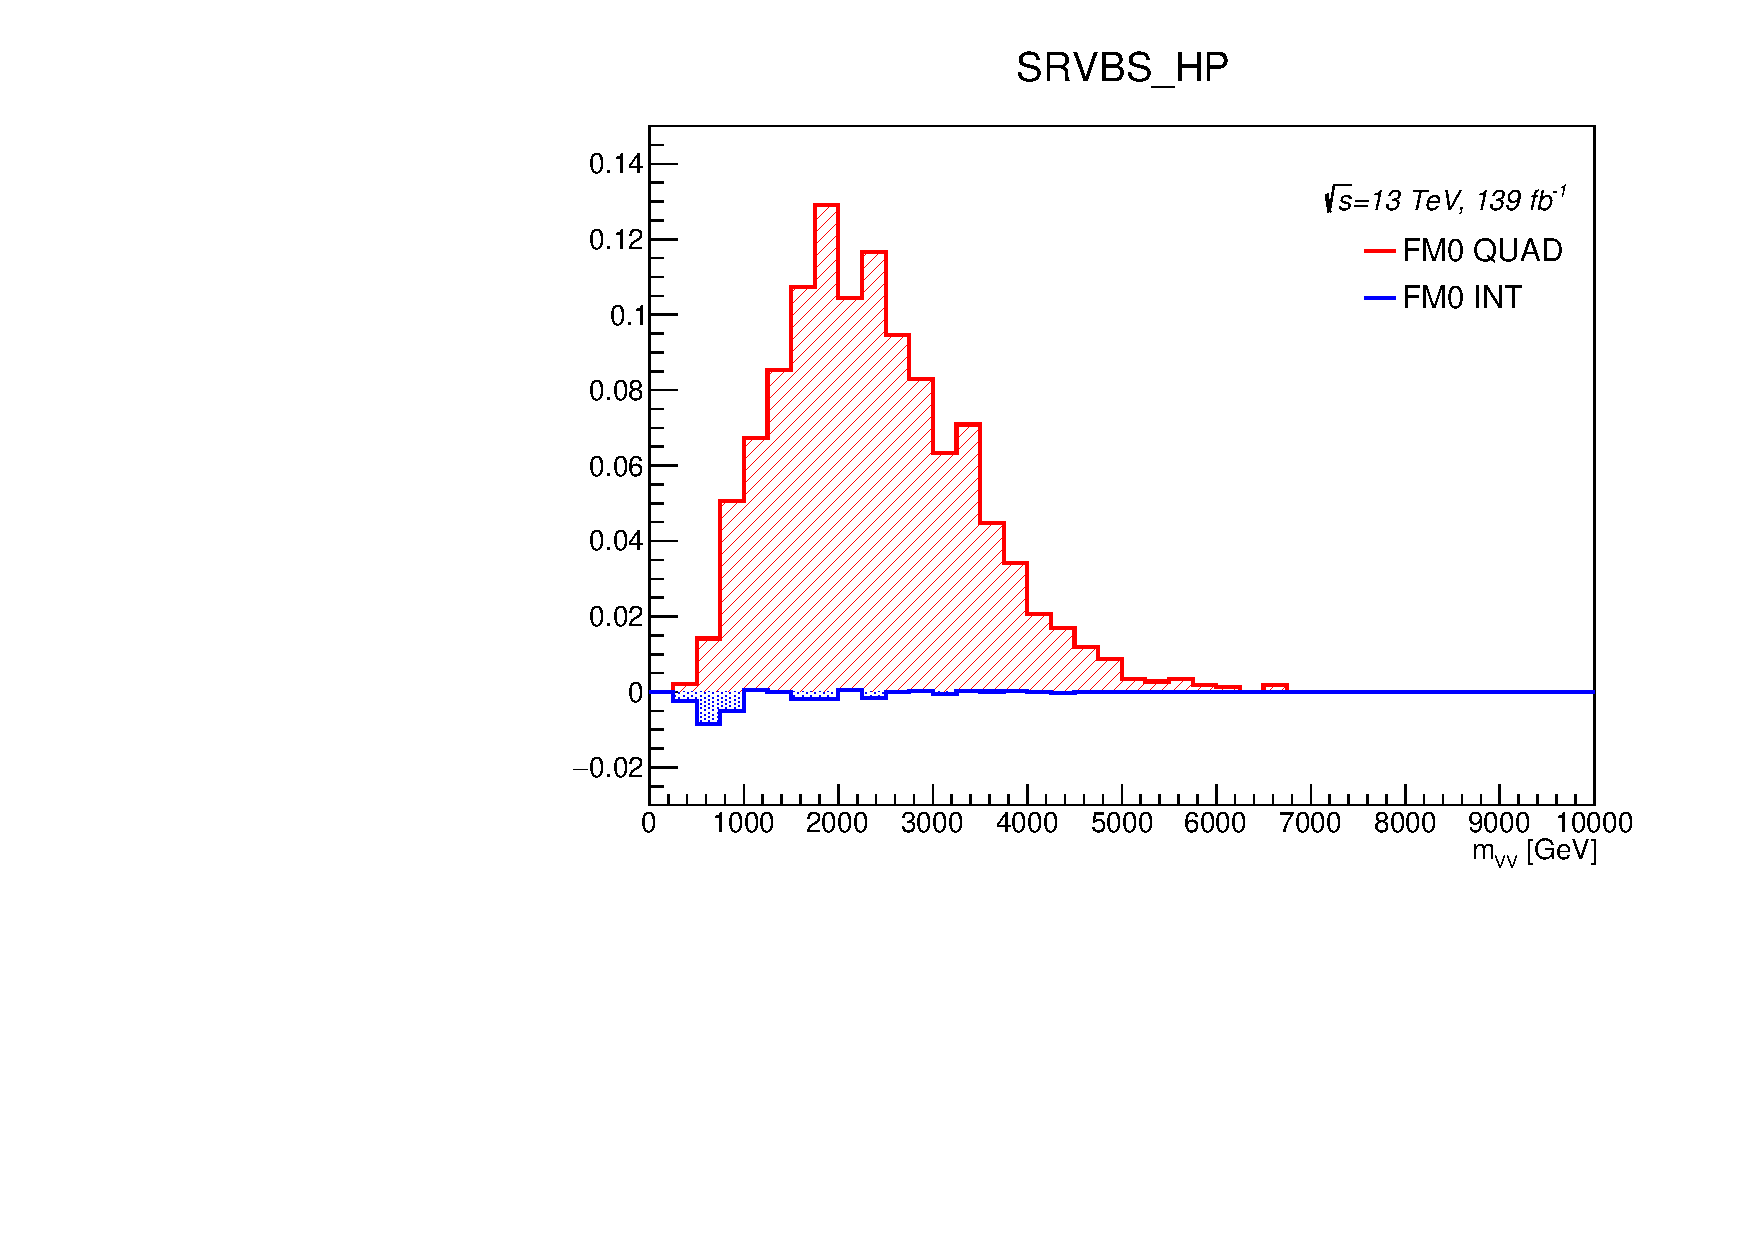
\includegraphics[width=0.45\textwidth]{figures/aQGC/FM0_0ptag1pfat0pjet_0ptv_SRVBS_HP_MllJ.pdf}
        \caption{The comparison of the quadratic term and the interference term with FT0 (top left), FS02 (top right), and FM0 (bottom middle) in 2-lepton channel HP SR. The contribution of the interference term can be negative, and it is larger in FS terms. The signal sample is produced at $\frac{f_i}{\Lambda^4} = 1~[\mathrm{TeV}^{-4}]$. }
        \label{fig:quadint}
\end{figure}
For the purpose of excluding a signal hypothesis, confidence intervals are derived to set limits. 
Confidence intervals are calculated with asymptotic formulae using Wilks' theorem~\cite{10.1214/aoms/1177732360}, assuming that the profile likelihood test statistic follows $\chi^2$ distribution~\cite{Cowan:2010js}.
%Explaing the definition of test statistic
%The test statistic is 

\section{Clipping method}
\label{subsec:clipping}
As the EFT may violate unitarity at a large energy scale, the clipping method, mentioned in section~\ref{subsec:EFT}, is used to study the range of cut-off scale that the experimental result can give limits on perturbatively calculable models.
%to preserve the unitarity at high center of mass energies. 
The EFT signal is set to zero at truth $m_{VV} > E_{clip}$, where the $E_{clip}$ is [1.5, 2, 3, 5, $\infty$]~TeV. 
%These five clipping points are chosen so that we can compare the results with other channels or experiments, as recommended from the anomalous gauge couplings (aGC) taskforce.~\cite{ATL-COM-PHYS-2017-433} 
%Figure~\ref{fig:clipped} shows how the $m_{VV}$ is shown at the low clipping energy.
The background samples, which are all standard model predictions, are not clipped.
The expected and observed limits are obtained with all 3 channels at each of the clipping points and compared with the theoretical unitarity bound.
\section{Study of final discriminant in aQGC search}
\label{subsec:2binapproach}
The aQGC terms can modify the amplitude of the VBS process at the higher effective center-of-mass energy, $m_{VV}$, as shown in Figure~\ref{fig:2lepaQGCshapeMVVh}.
It is found that the reconstructed $m_{VV}$ (or \mt\ in \zlep\ channel) is the best variable to separate the aQGC signals from the all SM processes, while it cannot separate the SM EW VV+jj process from the SM background as shown in figure~\ref{fig:2lepaQGCshapeMVVh}.
The RNN score distributions for the aQGC samples are similar to the one for the SM electroweak signal and still useful to suppress the non-VBS background as shown in Fig.~\ref{fig:2lepaQGCshapeRNNh}.
\begin{figure}[]
    \centering
   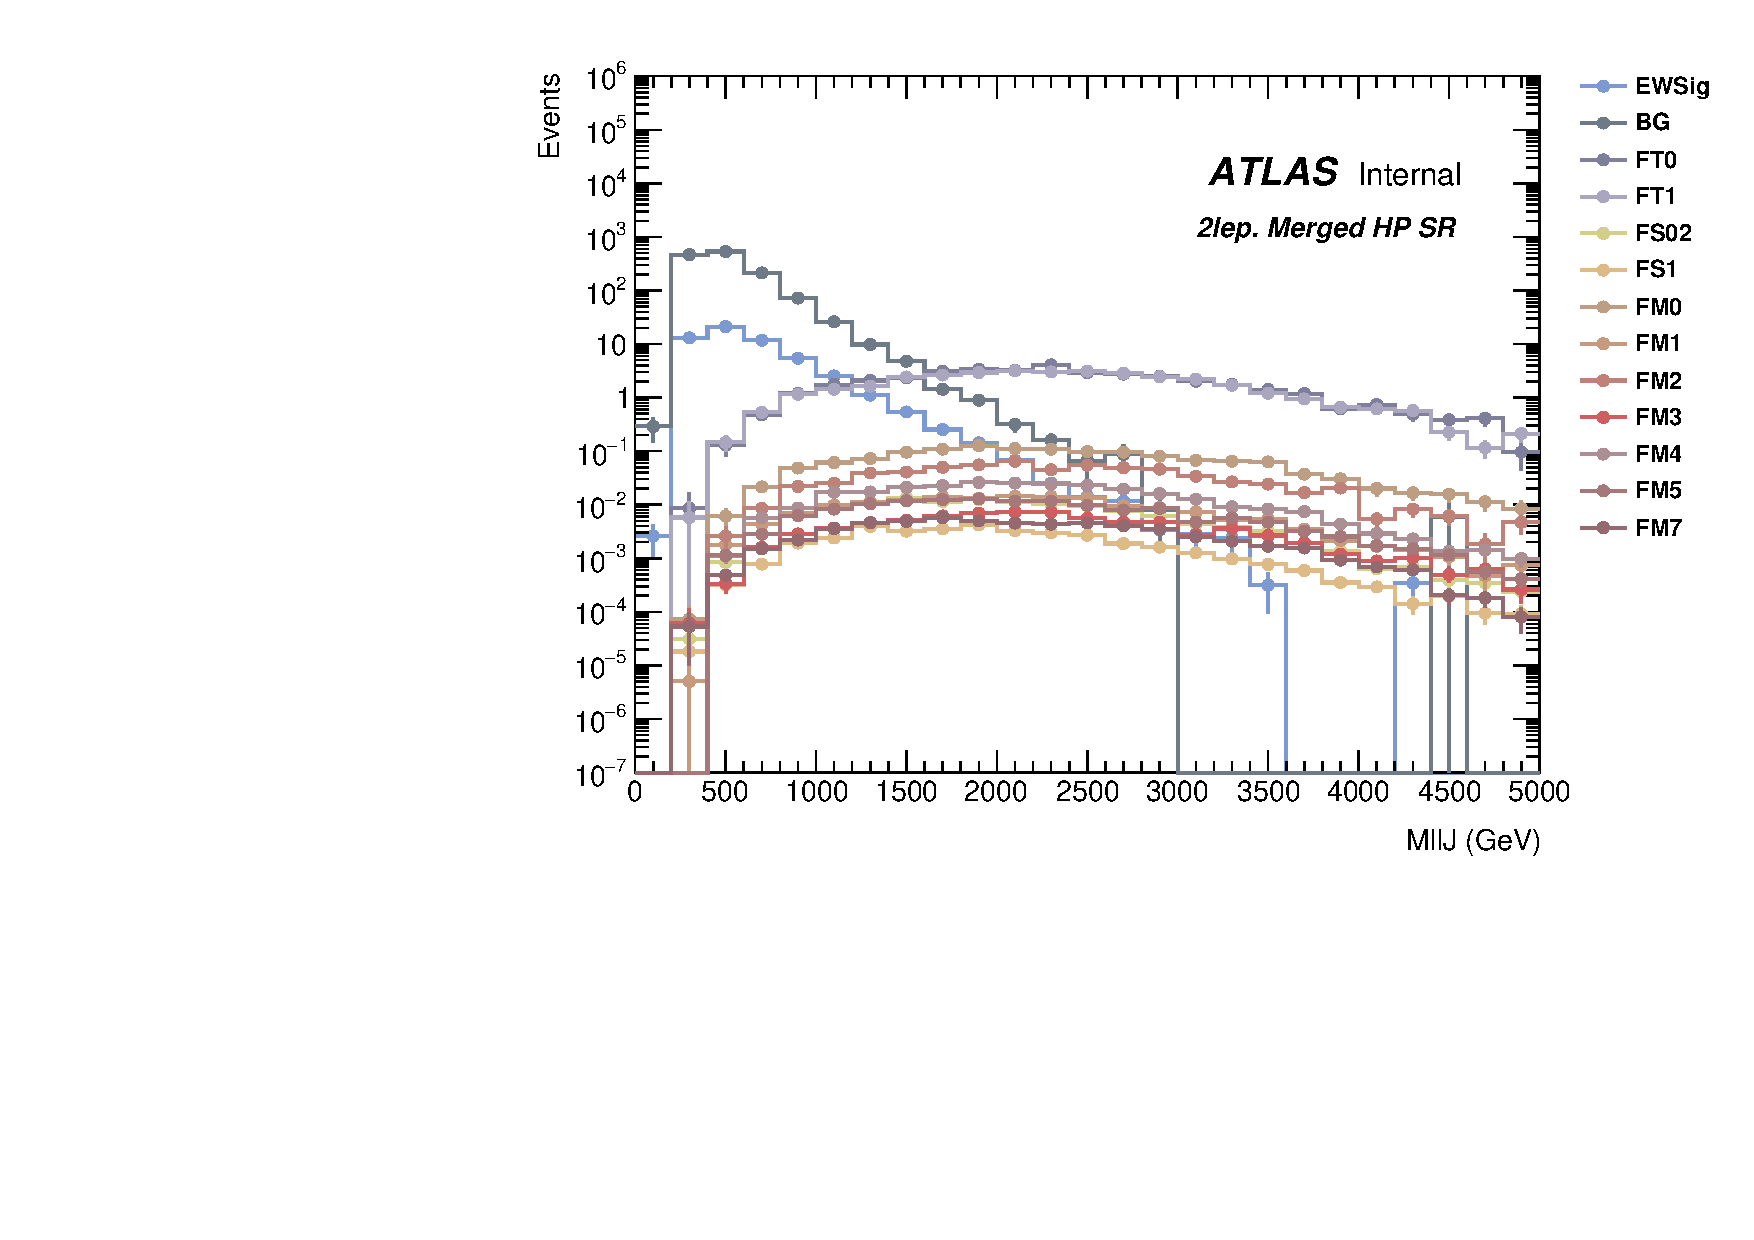
\includegraphics[width=0.45\textwidth]{figures/aQGC/MllJ_SR_HP_aQGC.pdf}
   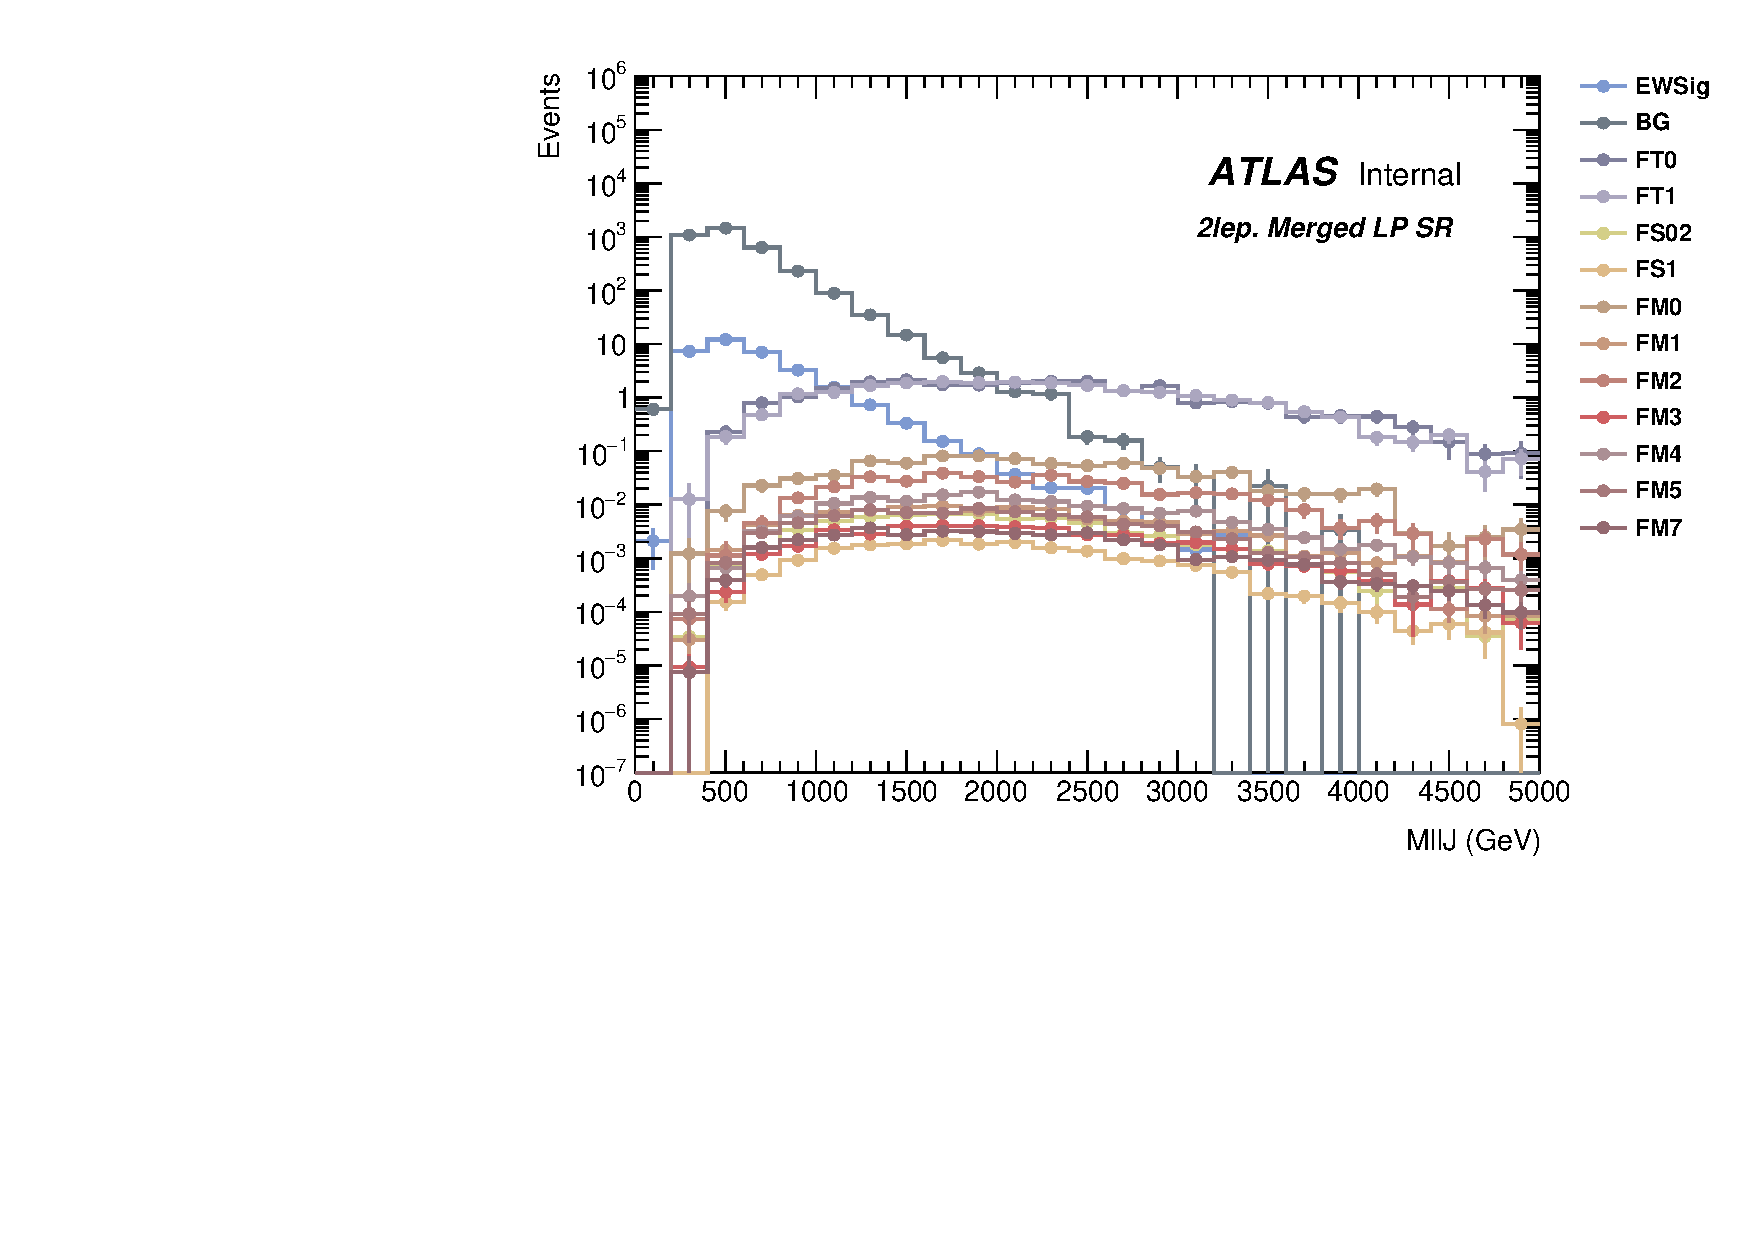
\includegraphics[width=0.45\textwidth]{figures/aQGC/MllJ_SR_LP_aQGC.pdf}
    \caption{$m_{VV}$ shape distribution of each Wilson coefficient in Merged Signal regions. Only quadratic terms are shown.}
    \label{fig:2lepaQGCshapeMVVh}
\end{figure}
\begin{figure}[]
    \centering
   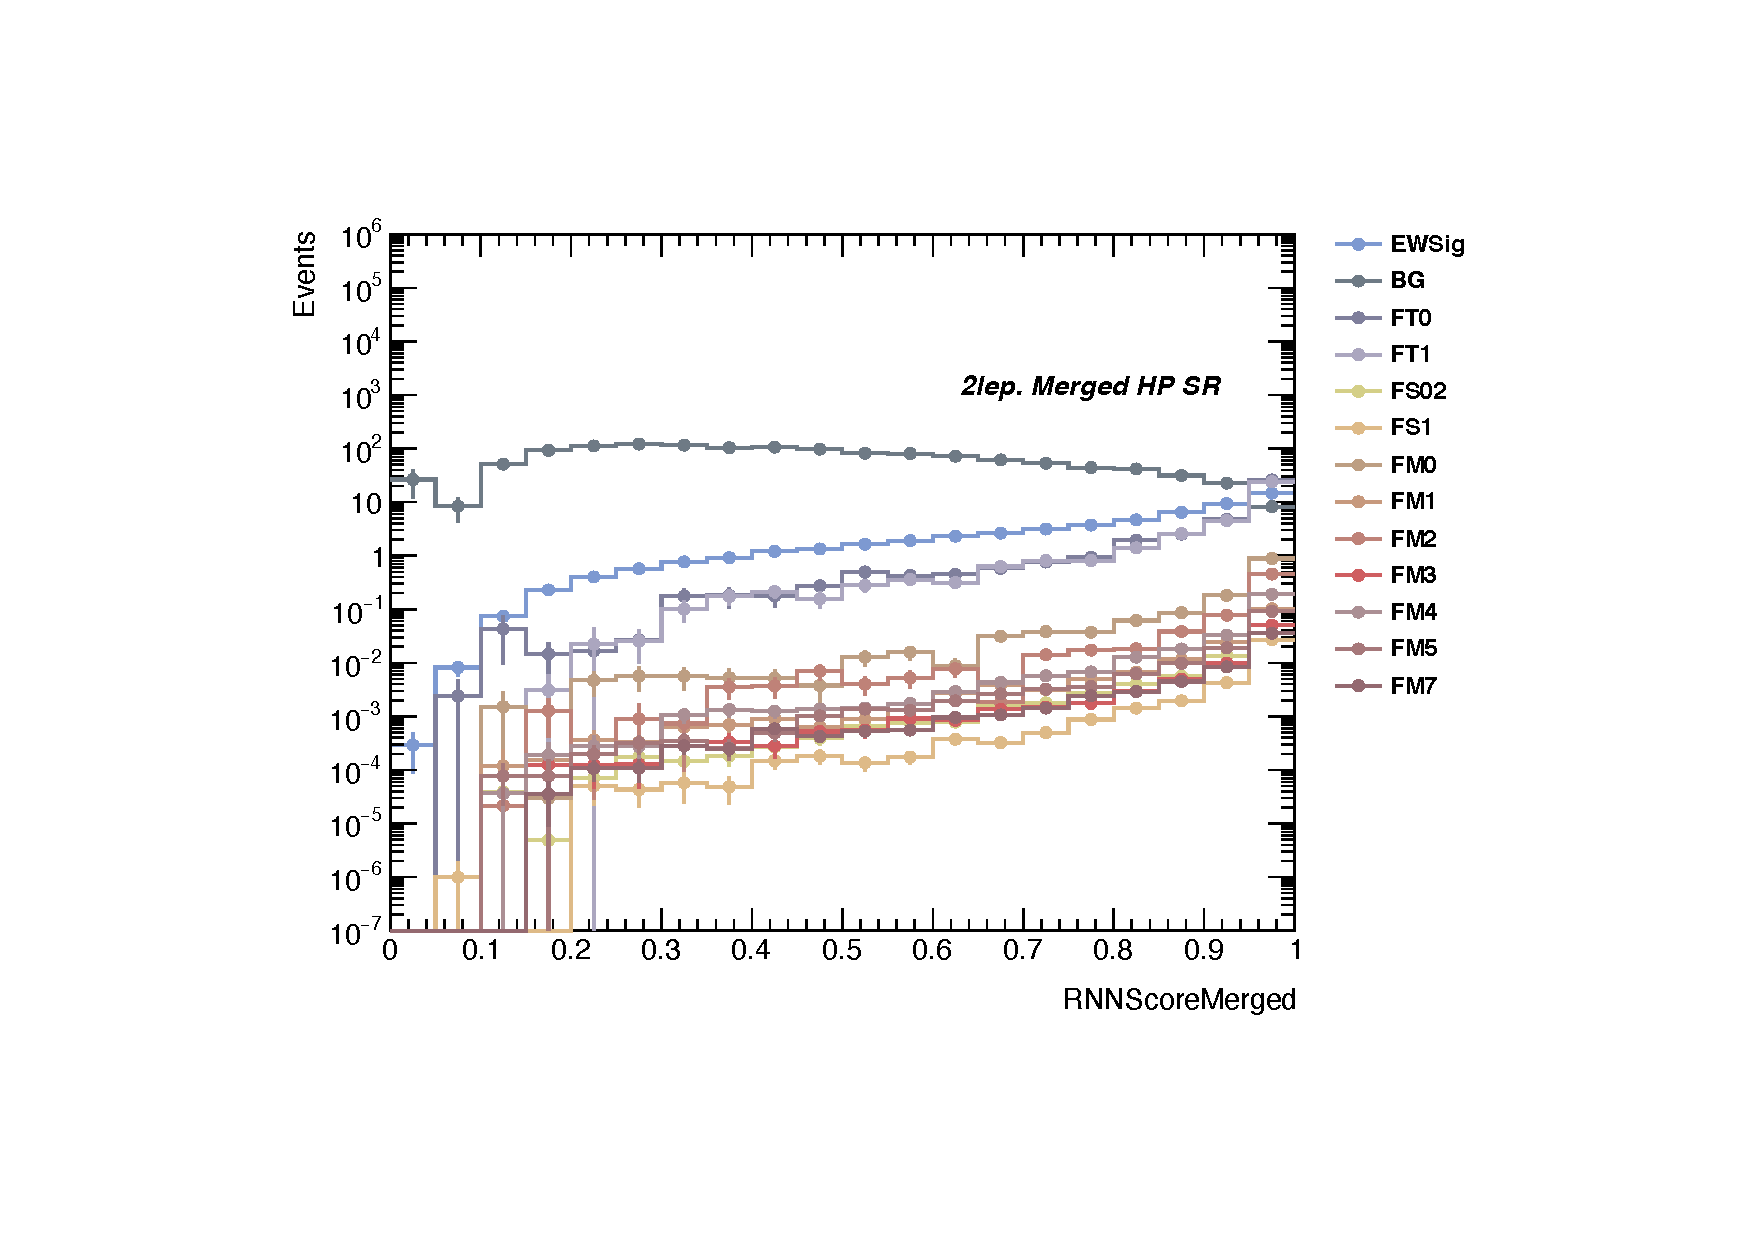
\includegraphics[width=0.45\textwidth]{figures/aQGC/RNNScoreMerged_SR_HP_aQGC.pdf}
   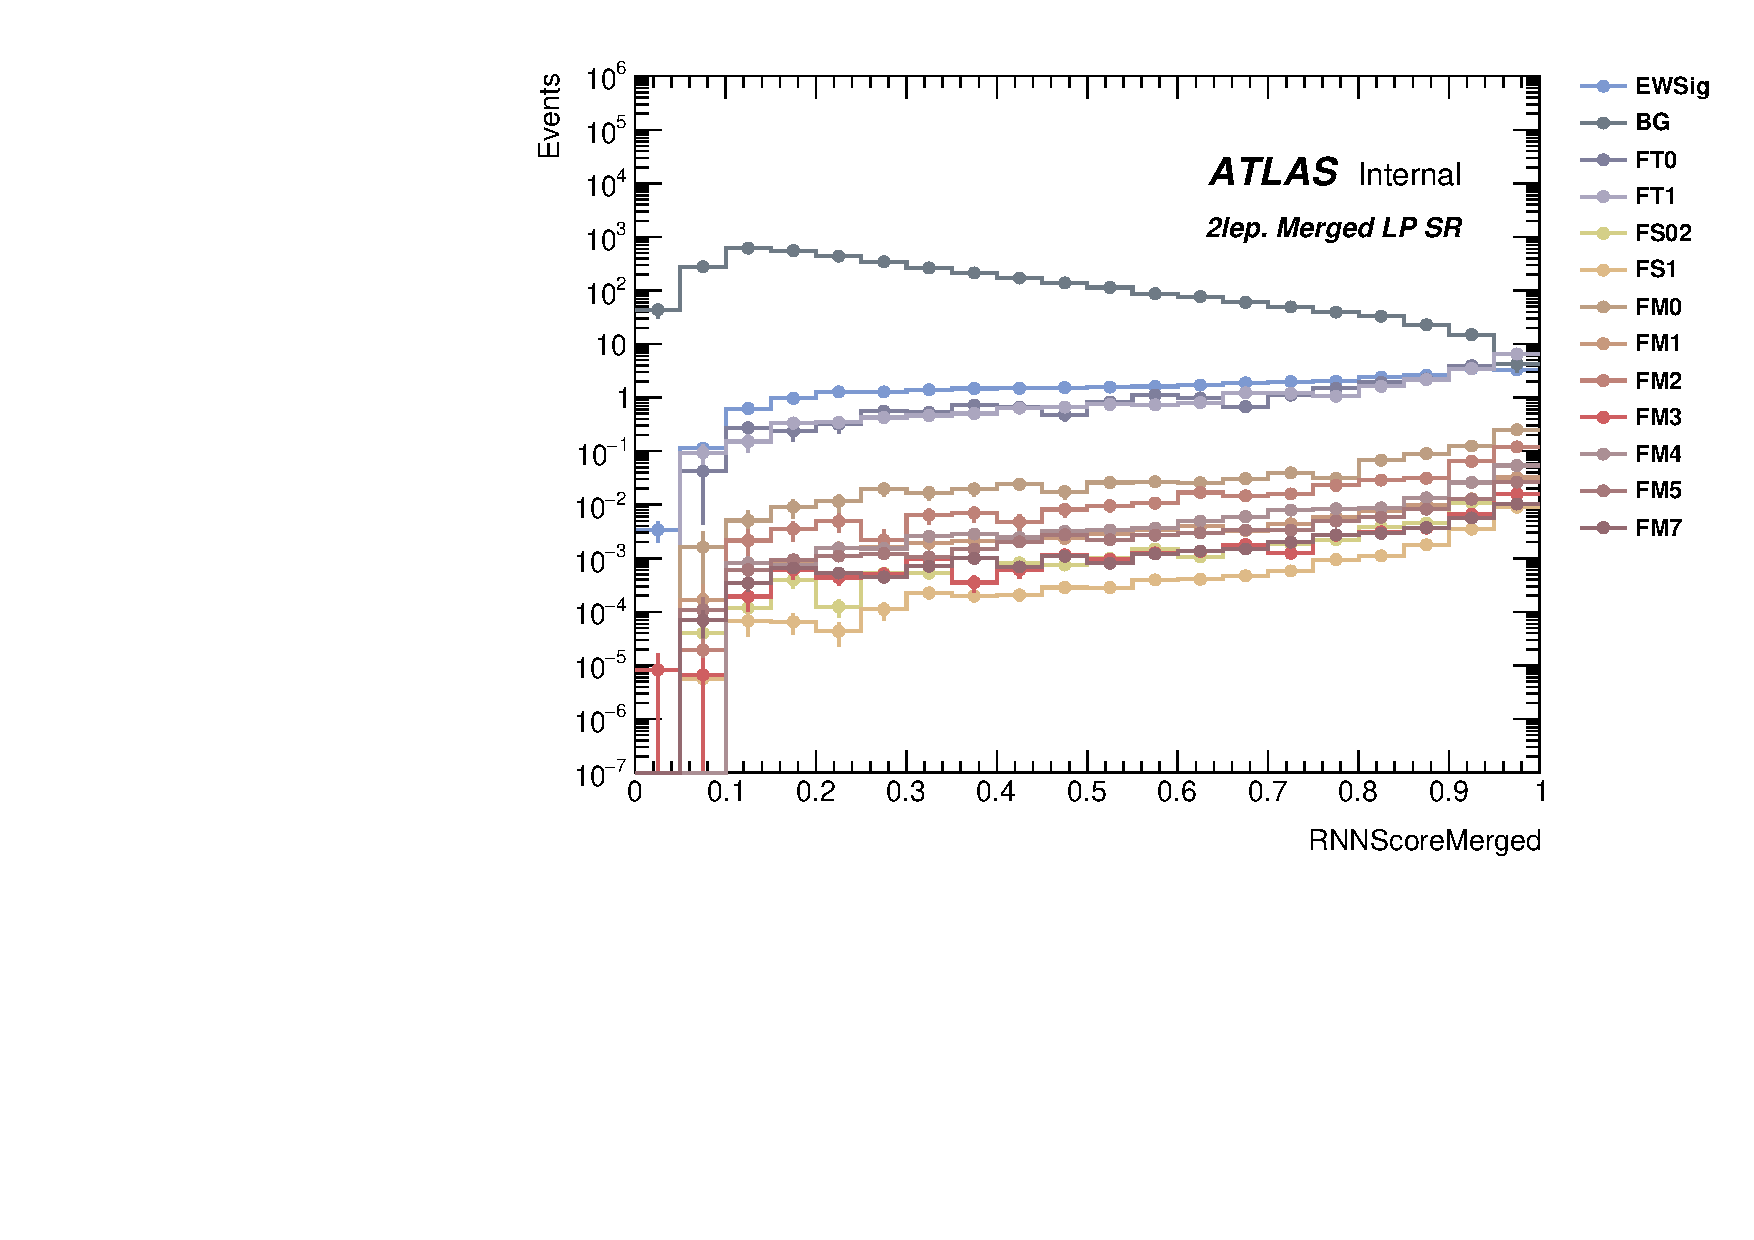
\includegraphics[width=0.45\textwidth]{figures/aQGC/RNNScoreMerged_SR_LP_aQGC.pdf}
    \caption{RNN score shape distribution of each Wilson coefficient in Merged Signal regions. Only quadratic terms are shown.}
    \label{fig:2lepaQGCshapeRNNh}
\end{figure}
Finally we would like to separate aQGC signals from both SM electroweak signal and the SM non-VBS background.
So that the final discriminant can make use of the both separation power of $m_{VV}$ and the RNN score, ideally 2-dimensional likelihood fit using $m_{VV}$ and RNN score is the best option, but considering that number of bins deteriorates the stability of the fit, we briefly optimized the binning strategy.
%%%%%%
We found a fit to RNN score distributions after SRs are further separated into 2 bin $m_{VV}$ categories is usable enough.
Its sensitivity is comparable with a fit to $m_{VV}$ distribution.
The optimal threshold to separate the SRs may depends on the clipping energy.
The threshold value at each clipping value is scanned and checked the sensitivity in figure~\ref{fig:ThresholdScan}.
%we compared the results with the following conditions.
%The fitting results with the following conditions are compared:
%\begin{itemize}
%  \item A fit to $m_{VV}$ distribution as discriminant, without any cuts on the RNN score;
%  \item A fit to the RNN score distributions after
%        SRs are further separated into two subcategories: \\
%        Low $m_{VV}$ : $m_{VV}$ $< 2000$~GeV and \\
%        High $m_{VV}$ : $m_{VV}$ $\geq 2000$~GeV. \\
%\end{itemize}
%The threshold 2000~GeV is derived from figure~\ref{fig:2lepaQGCshapeMVVh}.
%With the second option, the number of SRs is twice as shown in Figure~\ref{fig:2lepTwoBin}.
%(binning??)
%Unconditional Asimov fit (The log-likelihood fit using Asimov dataset without fixing the $\mu$ value) by using FT0 signal in only \tlep\ channel is performed.
%Only quadratic term is used in this study.
%The systematic uncertainties are not included in the fitting here, just the floated normalization factor is considered.
%The Asimov data used here is constructed from the background plus SM electroweak VV+jj signal samples.
%The expected limits and uncertainty of the expected signal strength of FT0 signal are shown in table~\ref{tab:2binlimit}.
%Significantly better upper limit on the signal strength is obtained by the second option (a fit to RNN score with the categorization by $m_{VV}$)
%than the first option (a fit to $m_{VV}$ distribution).
%The signal strength obtained by the second option (a fit to RNN score with the categorization by $m_{VV}$) and the first option (a fit to $m_{VV}$ distribution) is the same. 
%We found the first option cannot give any constraints on the SM electroweak VV+jj signal.
%It can be a motivation to use the RNN score also in the aQGC search study.

%\begin{figure}[ht]
%    \centering
%    	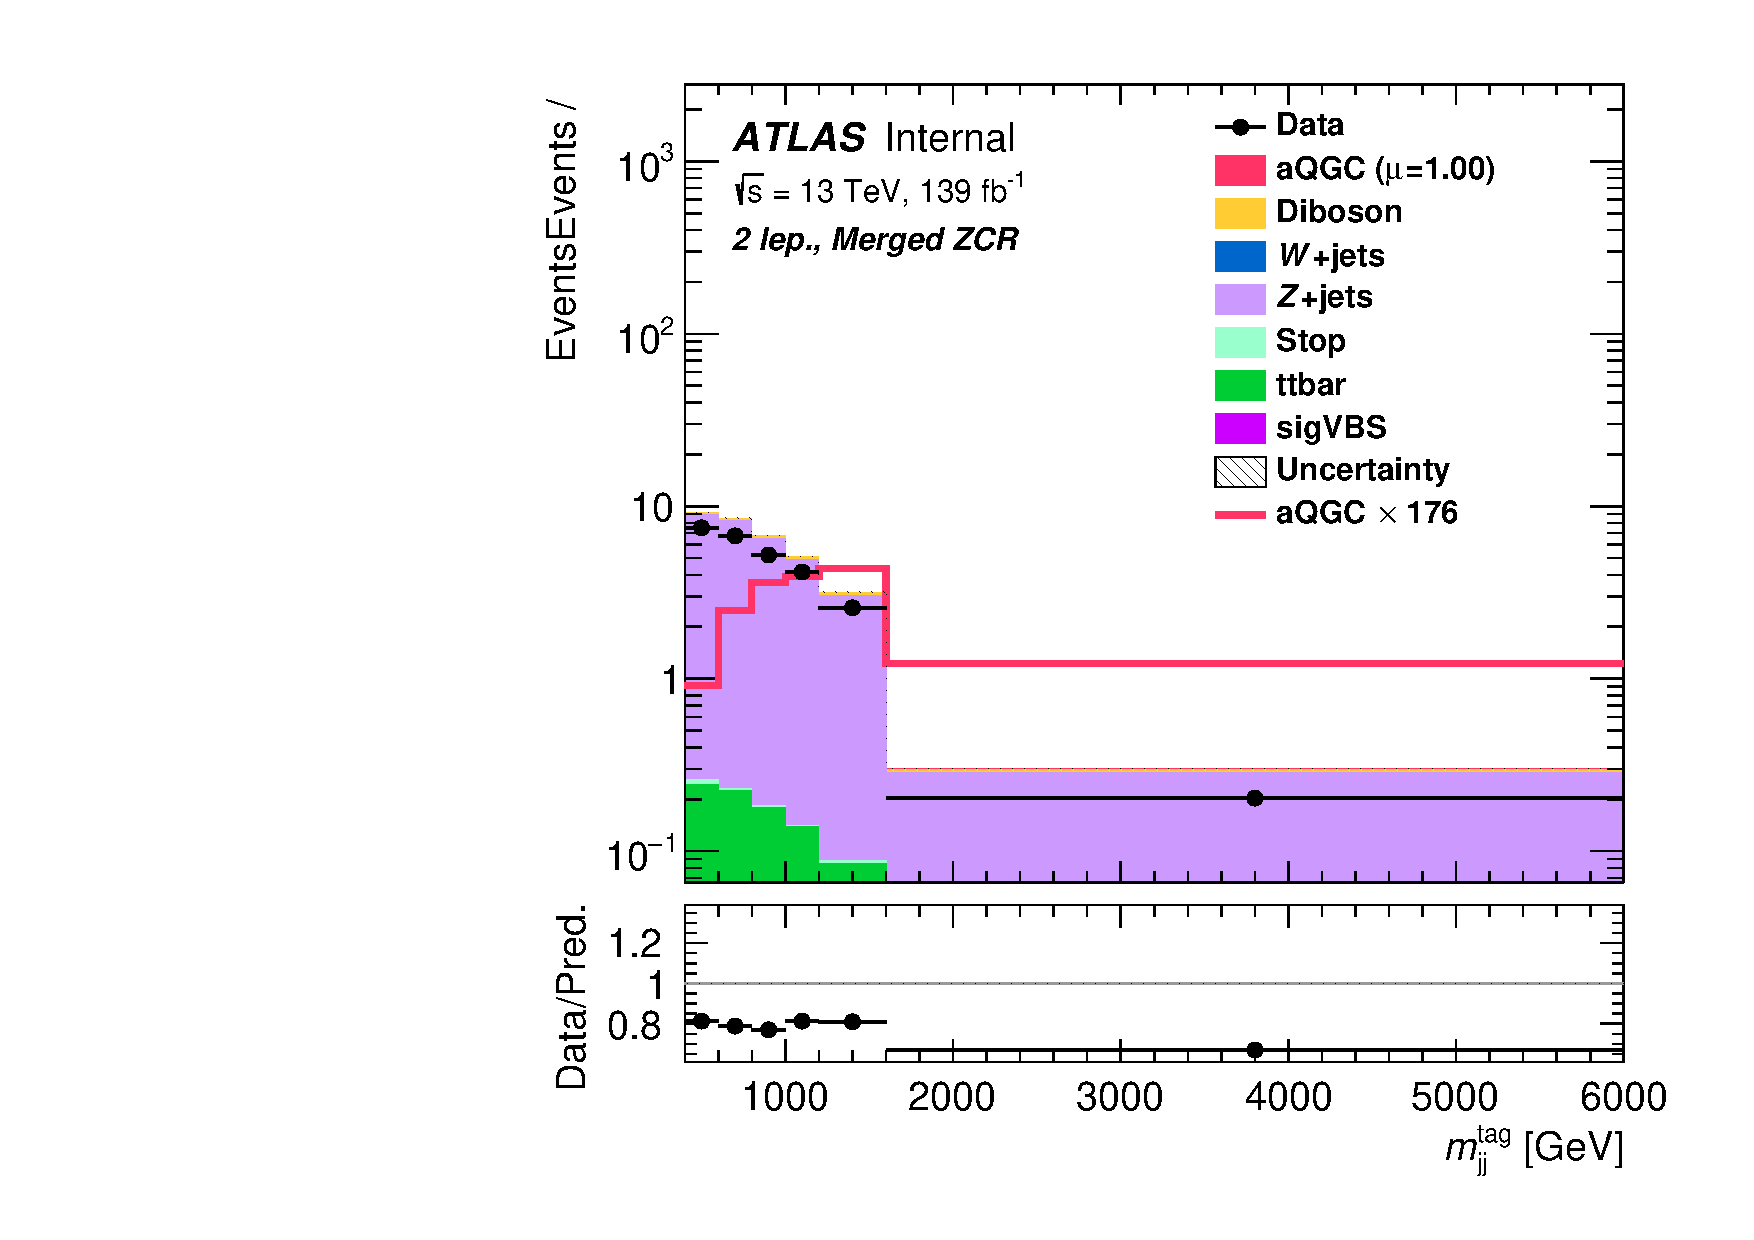
\includegraphics[width=0.32\textwidth]{figures/aQGC/Region_distMTagMerJets_DCRVjet_BMin0_J0_incJet1_L2_T0_incFat1_Y6051_incTag1_Fat1_Prefitlog.pdf}
%    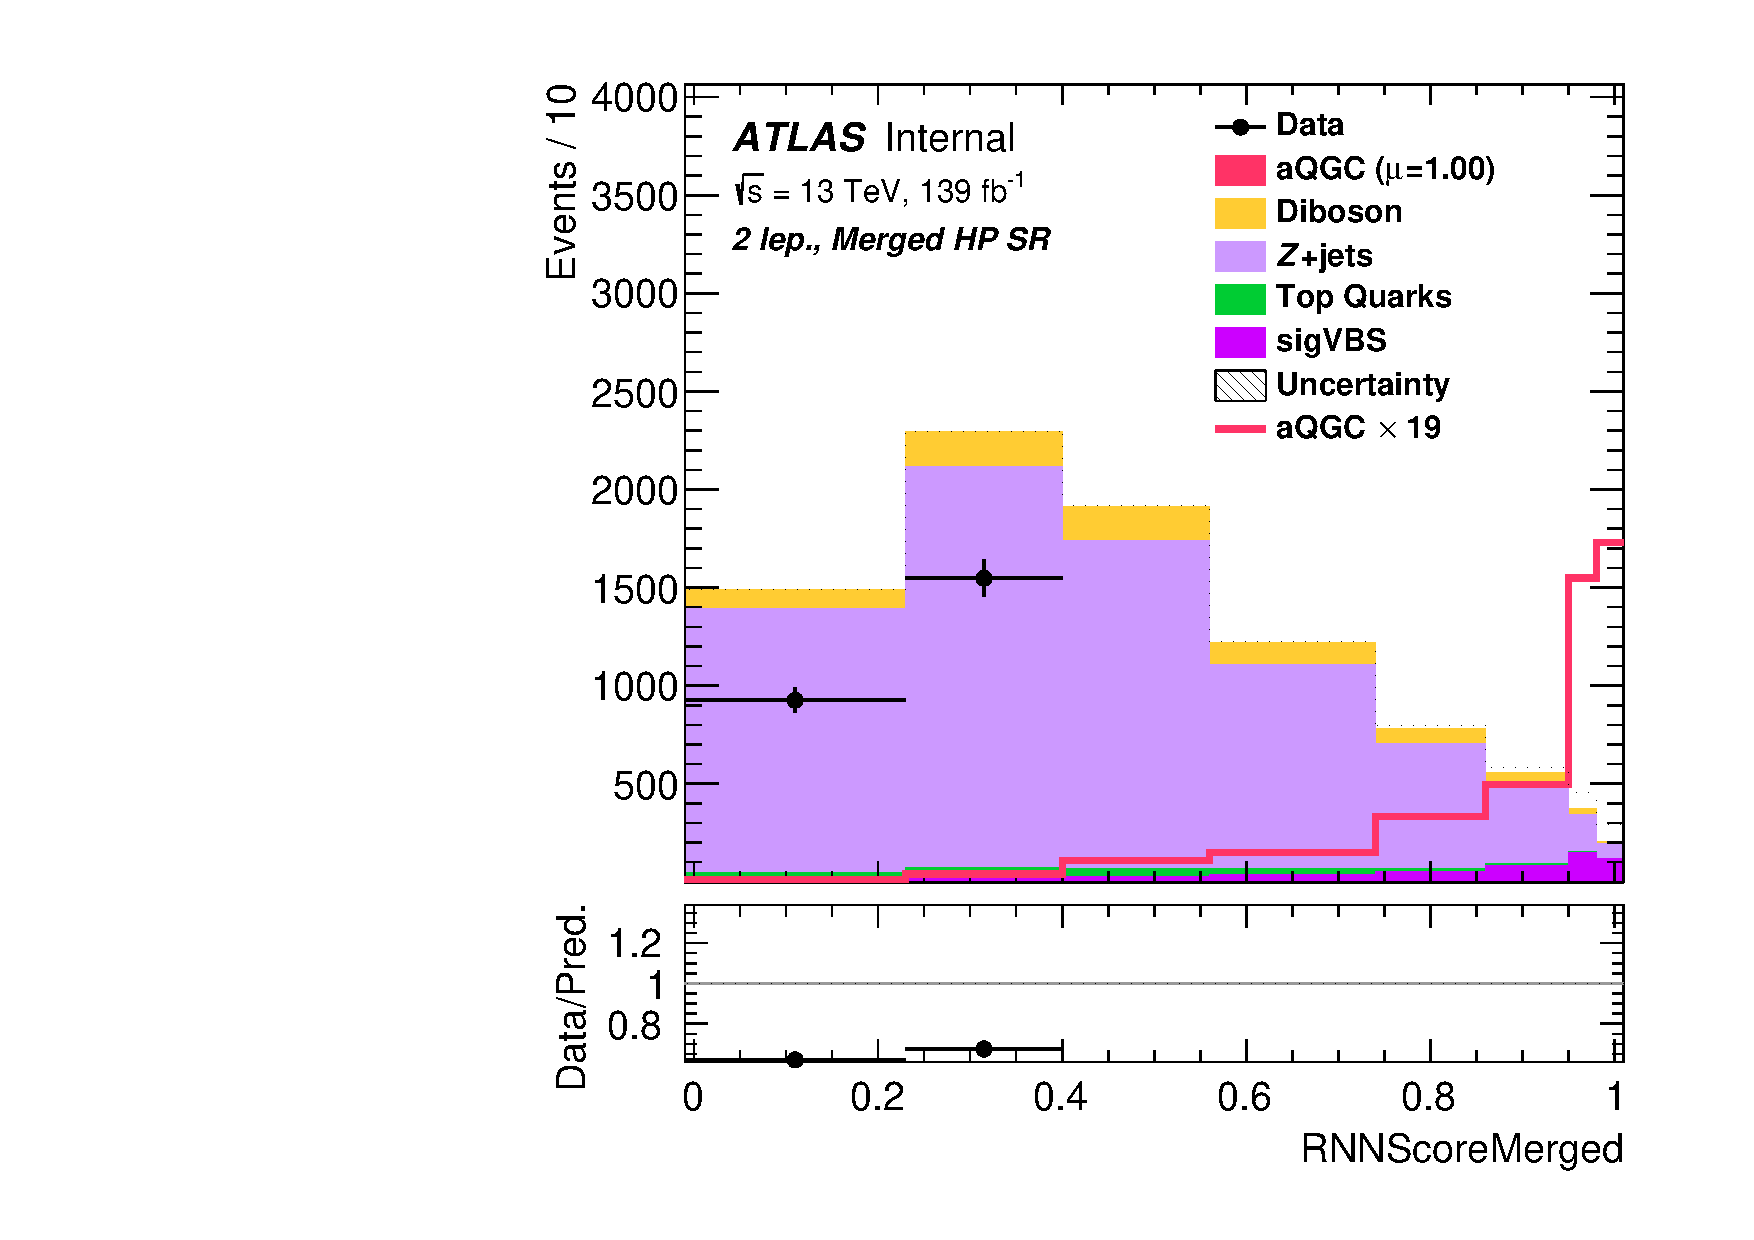
\includegraphics[width=0.32\textwidth]{figures/aQGC/Region_distRNNScoreMerged_DSRVBSHPLMVV_BMin0_J0_incJet1_L2_T0_incFat1_Y6051_incTag1_Fat1_Prefit.pdf}
% 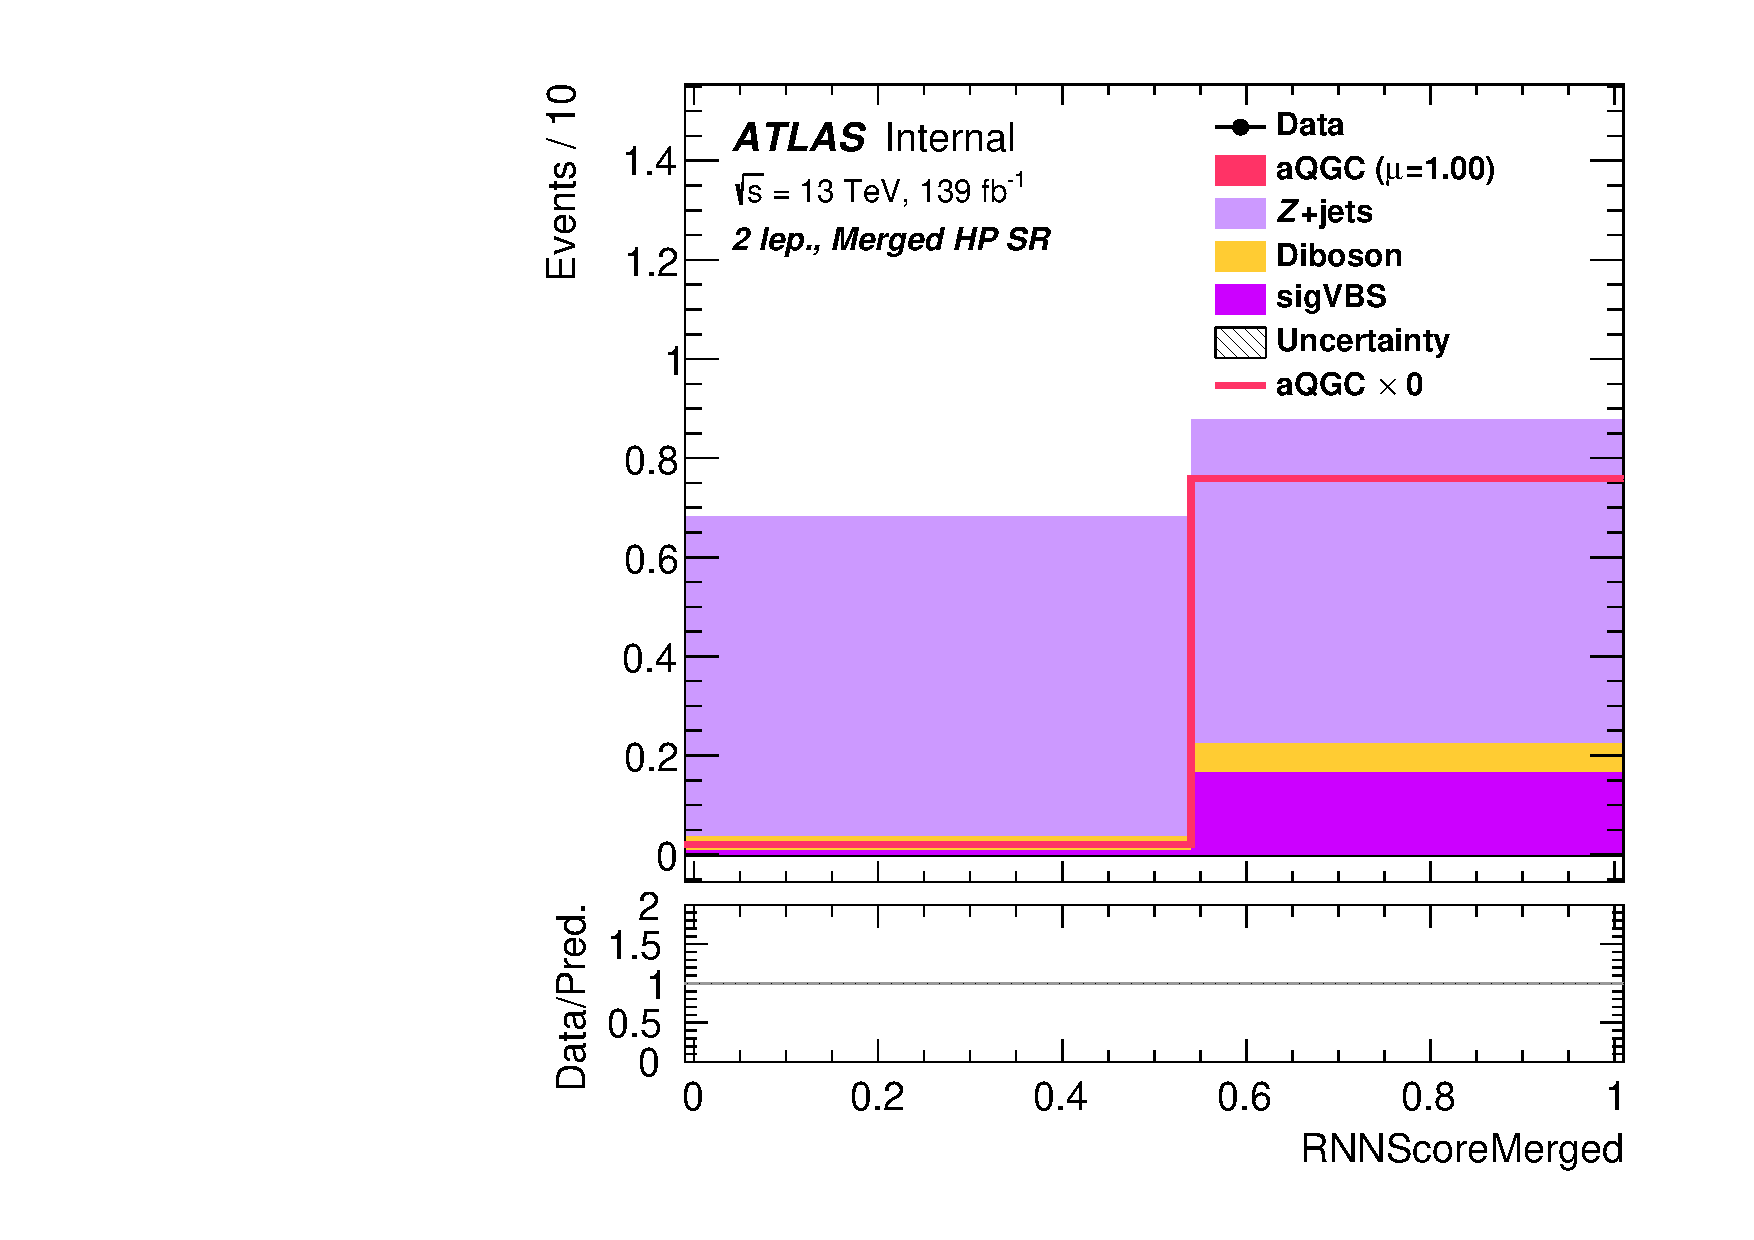
\includegraphics[width=0.32\textwidth]{figures/aQGC/Region_distRNNScoreMerged_DSRVBSHPHMVV_BMin0_J0_incJet1_L2_T0_incFat1_Y6051_incTag1_Fat1_Prefit.pdf}
%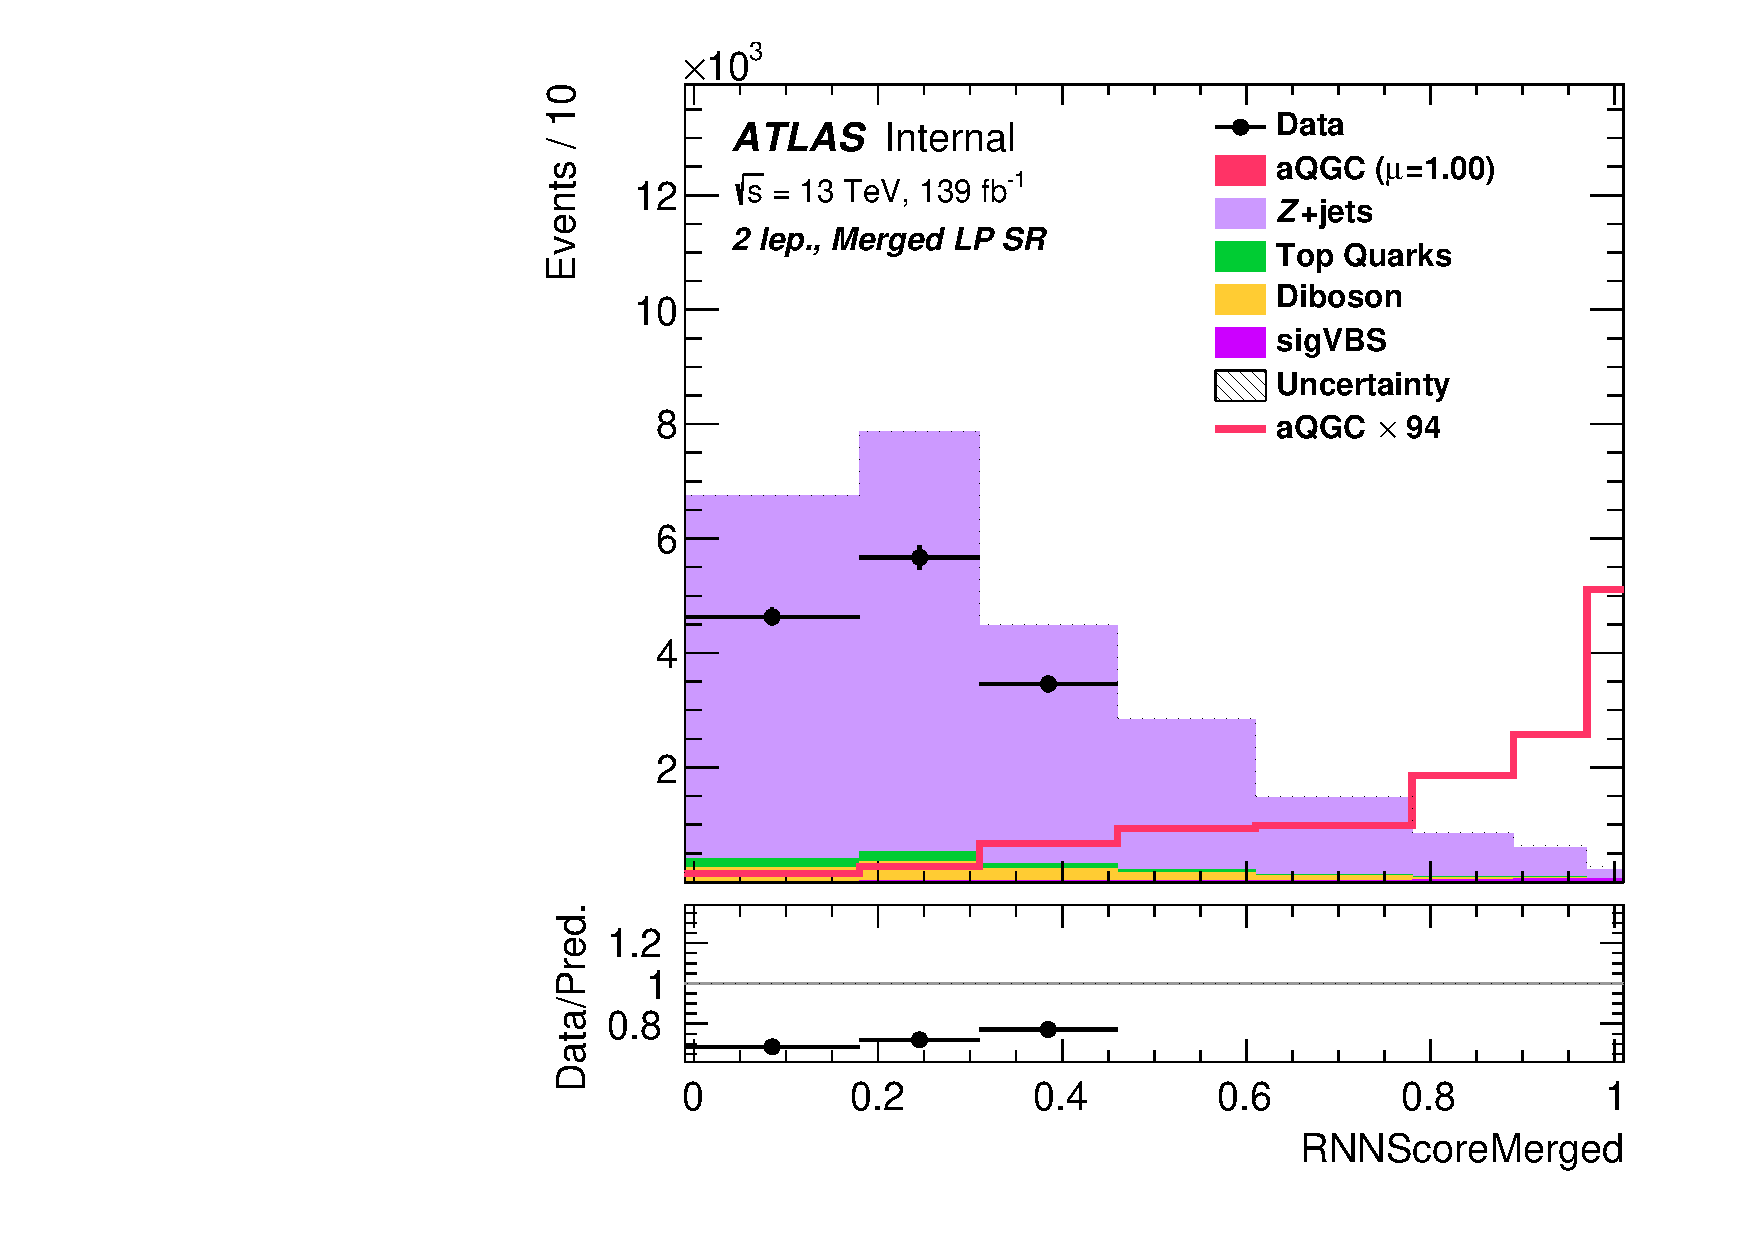
\includegraphics[width=0.32\textwidth]{figures/aQGC/Region_distRNNScoreMerged_DSRVBSLPLMVV_BMin0_J0_incJet1_L2_T0_incFat1_Y6051_incTag1_Fat1_Prefit.pdf}
%    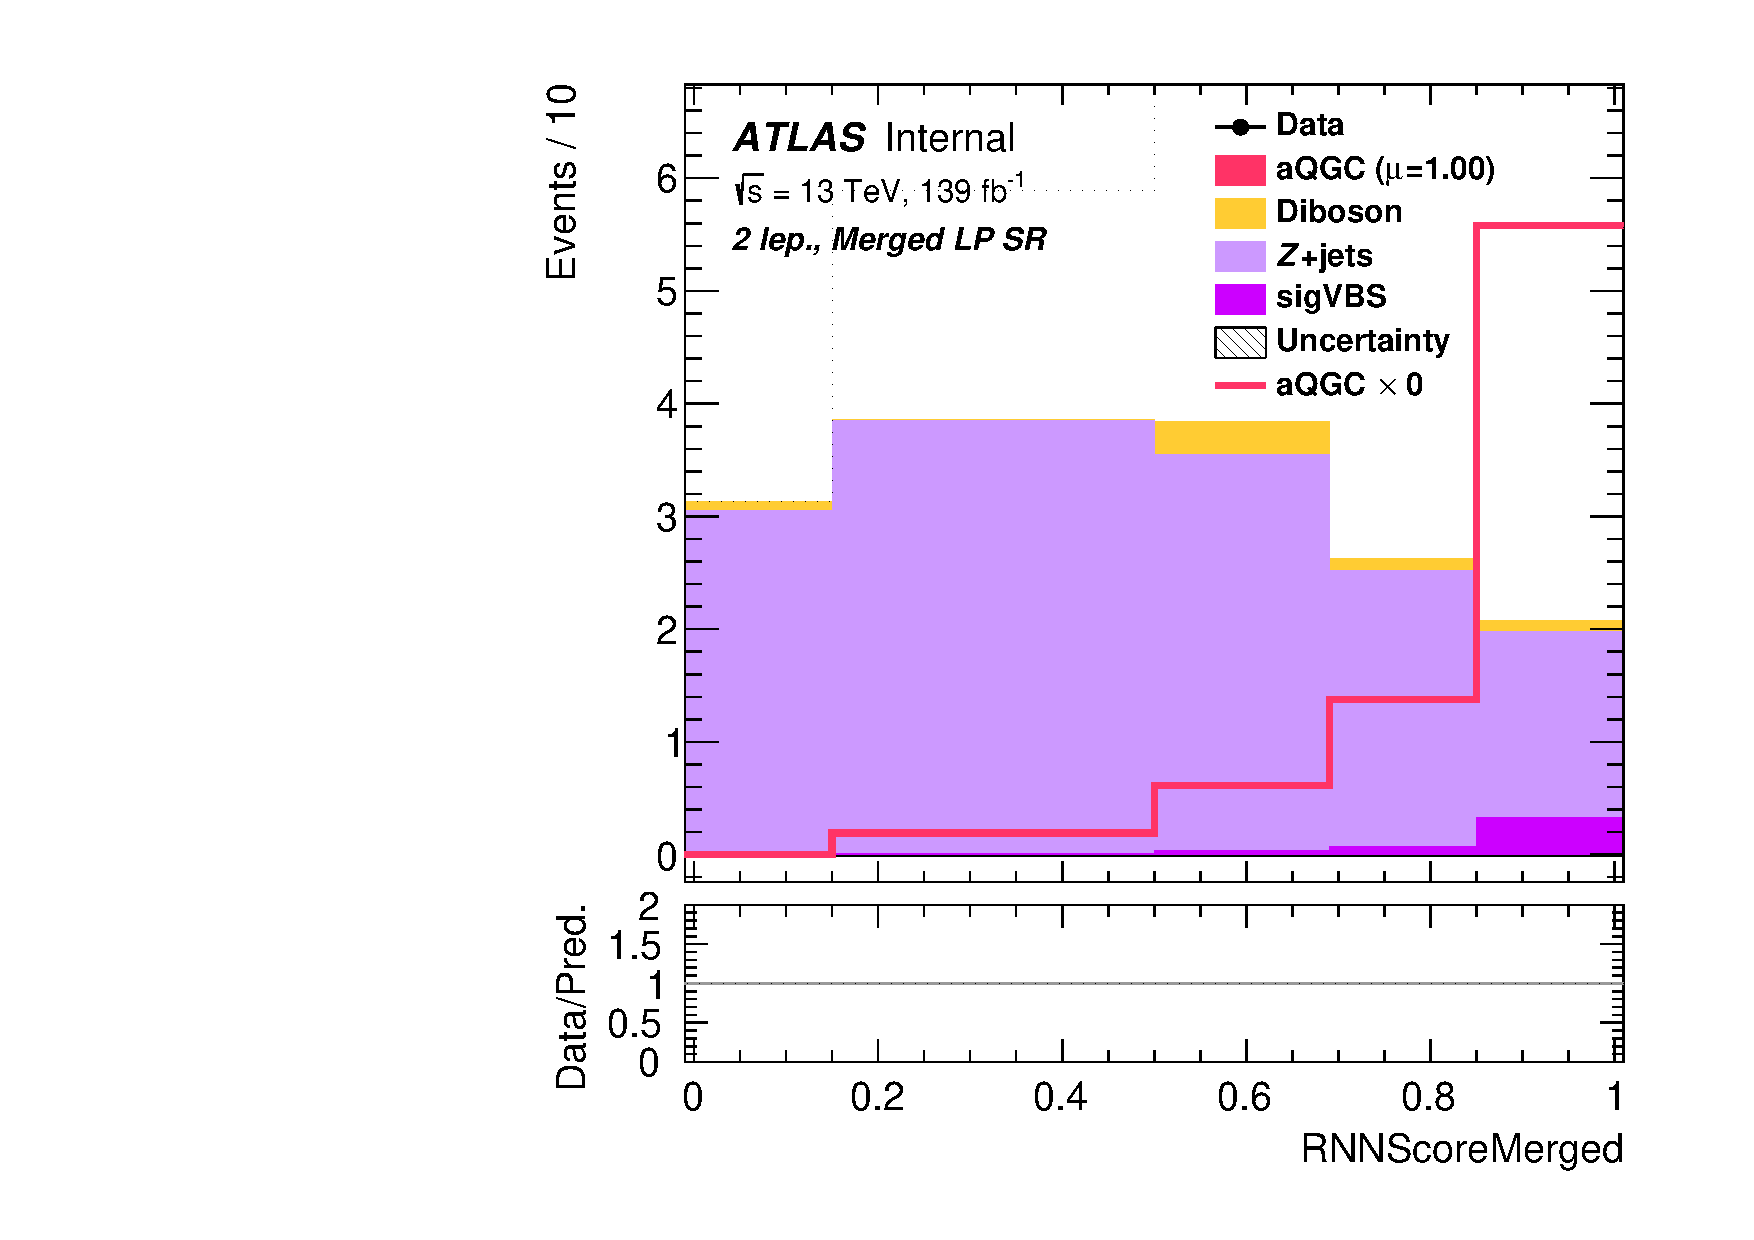
\includegraphics[width=0.32\textwidth]{figures/aQGC/Region_distRNNScoreMerged_DSRVBSLPHMVV_BMin0_J0_incJet1_L2_T0_incFat1_Y6051_incTag1_Fat1_Prefit.pdf}
%        \caption{Prefit plots for 2-bin strategy are shown. The RNN score is used as a discriminant for signal regions. operator FT0 in \tlep\ channel are shown. The standard model EW signal is floated as the background.}
%        \label{fig:2lepTwoBin}
%\end{figure}

%\begin{table}[ht!]
%\small
%\begin{center}
%\resizebox{0.9\textwidth}{!}{
%\begin{tabular}{ | l || l | l | l |}
%\hline
%                                    & Fit to $m_{VV}$ w/o further categorization & Fit to RNN score w/o further categorization  & Fit to RNN scores in separated bins of low- and high-$m_{VV}$  \tabularnewline \hline
%Unconditional fitted $\mu$          & -2.7e-06 $\pm$ 0.067   & 3.38e-05 $\pm0.038$      & 3.35e-05 $\pm0.029$  \tabularnewline \hline
%Norm sigVBS                         & 1 $\pm$ 2.1            & 1 $\pm$ 0.94             & 1 $\pm$ 0.48         \tabularnewline \hline
%Norm Z                              & 1 $\pm$ 0.036          & 1 $\pm$ 0.029            & 1 $\pm$ 0.027        \tabularnewline \hline
%Norm VV                             & 1 $\pm$ 1.13           & 1 $\pm$ 0.71             & 0.99 $\pm$ 0.64      \tabularnewline \hline
%Expected limit of $\mu$             & 0.19                   & 0.72                     & 0.10                 \tabularnewline \hline
%Expected limit of Wilson coefficient & 0.44                   & 0.85                     & 0.32                 \tabularnewline \hline
%\end{tabular}
%}
%\caption{Expected signal strength and limits in every two options. only \tlep channel is used for the fit. The result for single bin fit with RNN is also shown as a reference. The normalization fitted for standard model signal, and Z and diboson backgrounds are shown as Norm in the table.}
%\label{tab:2binlimit}
%\end{center}
%\end{table}

%\begin{table}[ht!]
%\small
%\begin{center}
%\resizebox{\textwidth}{!}{
%\begin{tabular}{ | l || l | l | l |}
%\hline
%                                    & Fit to $m_{VV}$ w/o further categorization & Fit to RNN score w/o further categorization  & Fit to RNN scores in separated bins of low- and high-%$m_{VV}$  \tabularnewline \hline
%Unconditional fitted $\mu$          & 8.83e-06 $\pm0.032$    & 1.02e-04 $\pm0.34$       & 1.09e-05 $\pm0.028$  \tabularnewline \hline
%Norm sigVBS                         & 1 $\pm$ 1.08           & 1 $\pm$ 0.79             & 1 $\pm$ 0.41         \tabularnewline \hline
%Norm Z                              & 1 $\pm$ 0.012          & 1 $\pm$ 0.010            & 1 $\pm$ 0.01         \tabularnewline \hline
%Expected limit of $\mu$             & 0.11                   & 0.70                     & 0.11                 \tabularnewline \hline
%Expected limit of Wilson coefficient & 0.33                  & 0.84                     & 0.33                 \tabularnewline \hline
%\end{tabular}
%}
%\caption{Expected signal strength and limits in every two options. only \tlep~channel is used for the fit. The result for single bin fit with RNN is also shown as a reference. The normalization fitted for the standard model signal, and Z backgrounds are shown as Norm in the table.}
%\label{tab:2binlimit}
%\end{center}
%\end{table}

%\section{Optimization of the threshold of 2-bin approach}
%\label{subsec:aQGCbinninb}
%Of course, the optimal threshold of $m_{VV}$ can be different depending on the clipping energy.
%In addition, a fine-tuning of the $m_{VV}$ threshold might be needed by considering the stability of the background estimation.
%The expected limit is shown in each threshold for $m_{VV}$ of 1000~GeV, 1500~GeV, 2000~GeV for a variety of the clipping points in Figure~\ref{fig:ThresholdScan}.
As expected, a higher $m_{VV}$ threshold is preferred at the higher clipping point, while a lower $m_{VV}$ threshold is favored at the lower clipping point.
1500~GeV is chosen as the best compromise to separate SRs into low- and high-$m_{VV}$ bins for the 2-lepton channel.

Since the meaning of the actual $m_{VV}$ distributions used in each lepton channel are different,
(fully reconstructed system in the \tlep\ and in the \olep\, and transverse mass in the \zlep\ solving neutrino ambiguity )
the optimal thresholds to separate SRs into low- and high-$m_{VV}$ bins in \olep\ and \zlep\ channels are also studied and  determined in table~\ref{tab:2binthreshold}.
%In \olep\ channel, the same threshold as \tlep\ channel, 1500~GeV, is just chosen since the reconstructed $m_{VV}$ distribution is similar. 
%In \zlep\ channel, the threshold needs to be optimized, since it uses \mt\ instead of $m_{VV}$.
%As shown in Figure~\ref{fig:mVVdist} the \mt\ shape in \zlep\ channel is different from $m_{VV}$ in \tlep\ channel.
%Here, the background yield in each bin of the high-$\mt$ regions is adjusted to be more than 5 so that
%the asymptotic calculation of the sensitivity is ensured with a certain number of background events.
%The threshold finalized is shown in Table, for each lepton channel, and for each region.
%Only in \tlep\ channel, less than 5 background events are expected in the second bin of the HP signal region.
%We are going to test if the asymptotic formulae works fine, by running toy experiments [TO DO].
\begin{figure}[h]
        \centering
    	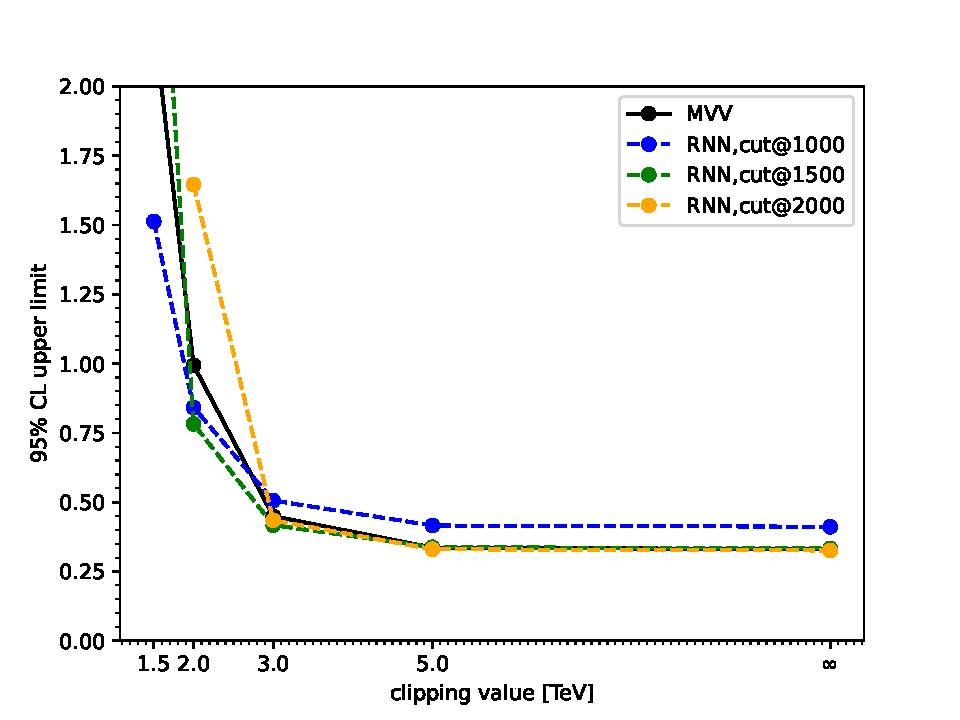
\includegraphics[width=0.50\textwidth]{figures/aQGC/ClippedFT02bin.pdf}
        \caption{Expected limits for 5 clipping points with each threshold for dividing $m_{VV}$ into 2 bins.}
        \label{fig:ThresholdScan}
\end{figure}
%\begin{figure}[ht]
%    \centering
%    	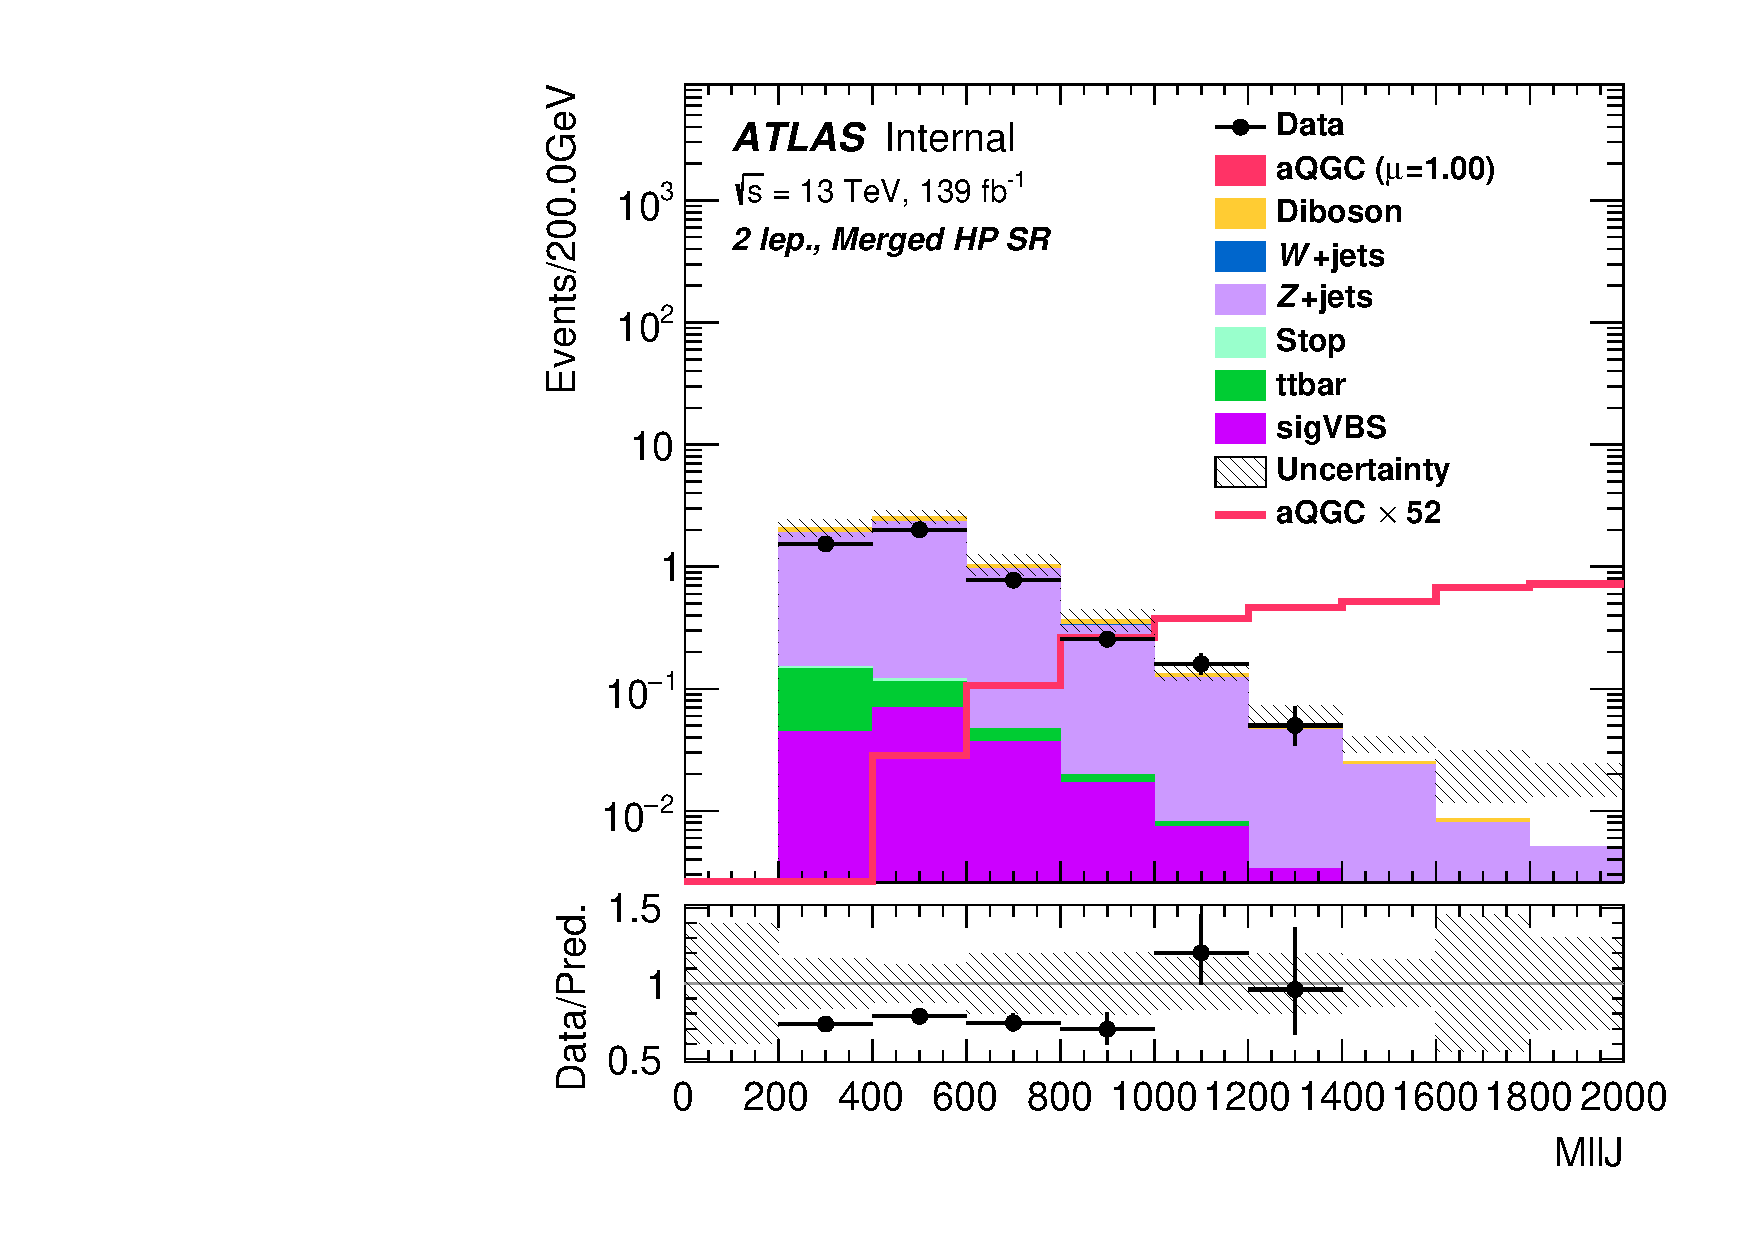
\includegraphics[width=0.32\textwidth]{figures/aQGC/MVV/Region_distMllJ_DSRVBSHP_BMin0_J0_incJet1_L2_T0_incFat1_Y6051_incTag1_Fat1_Prefitlog.pdf}
%    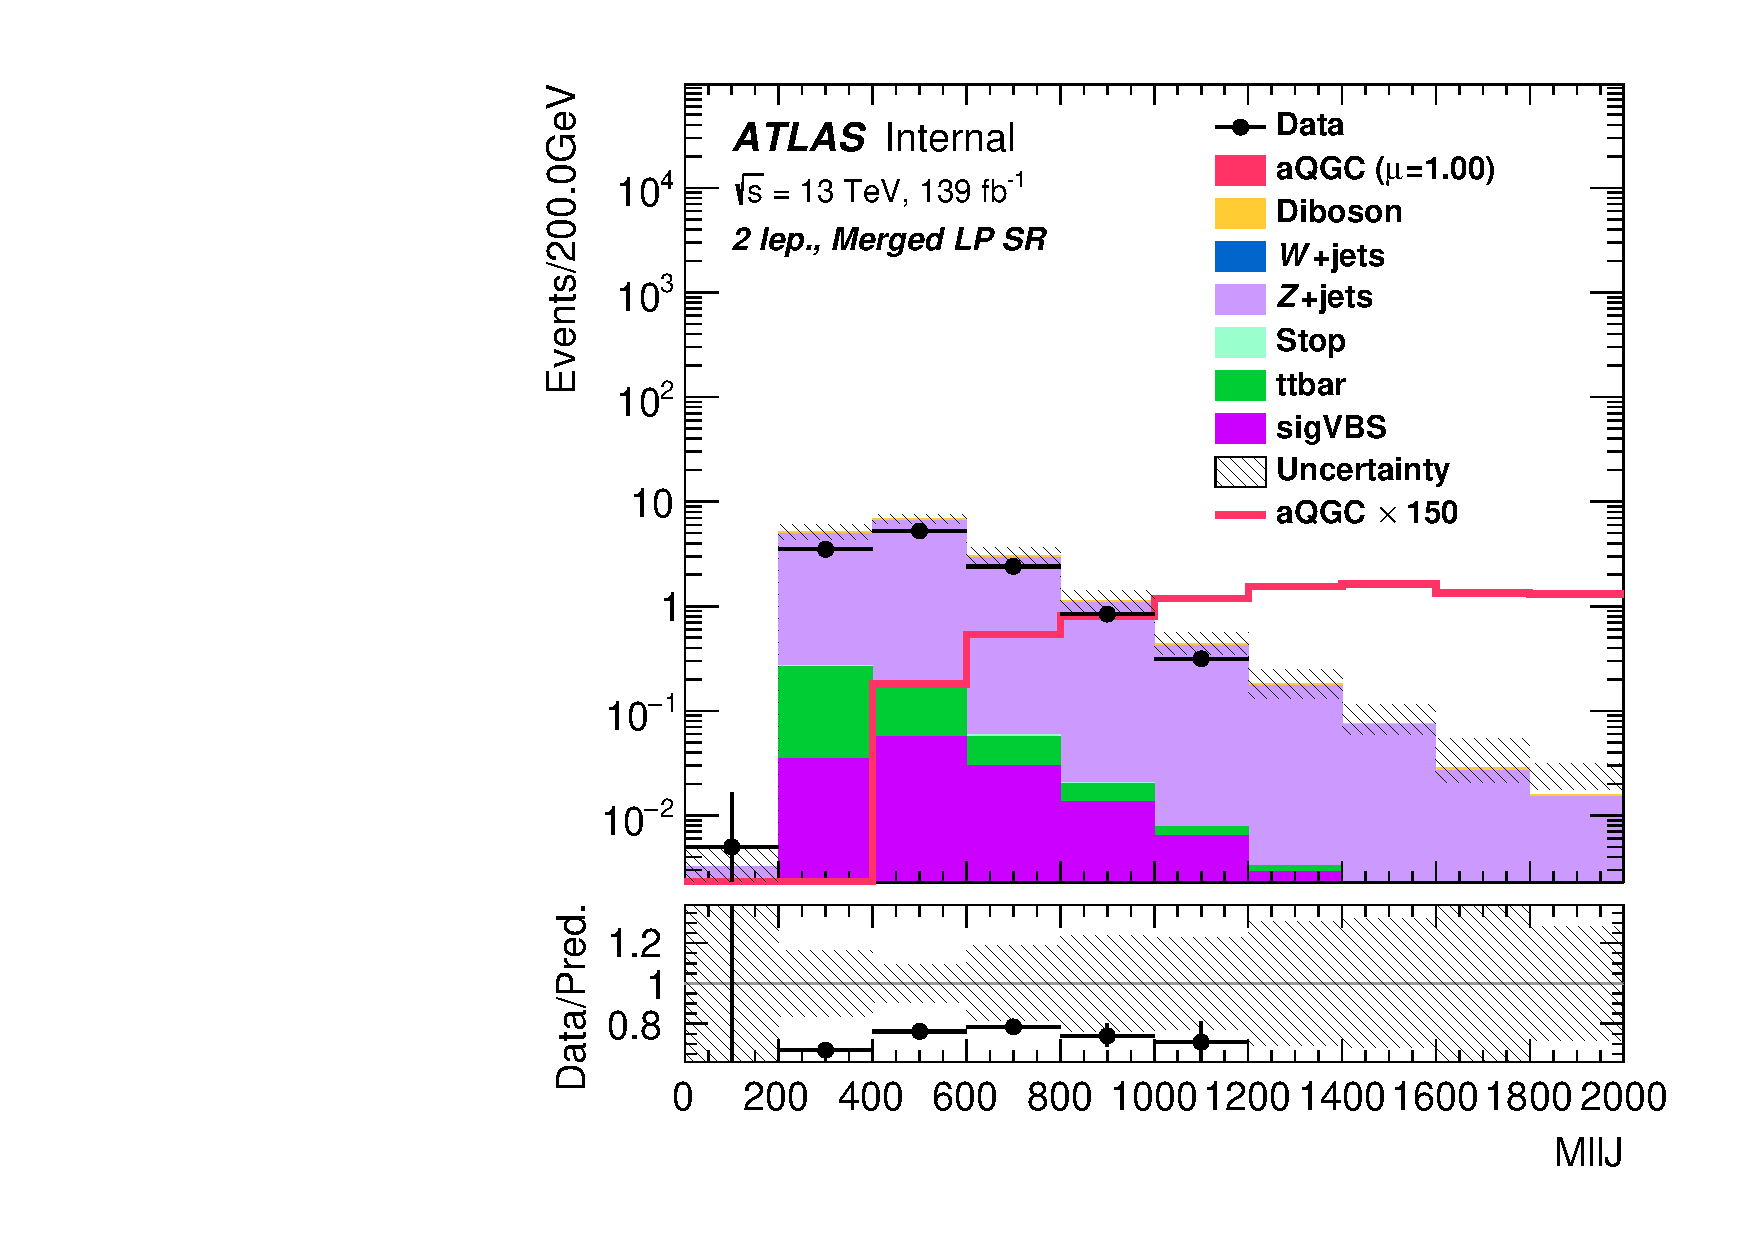
\includegraphics[width=0.32\textwidth]{figures/aQGC/MVV/Region_distMllJ_DSRVBSLP_BMin0_J0_incJet1_L2_T0_incFat1_Y6051_incTag1_Fat1_Prefitlog.pdf}
%  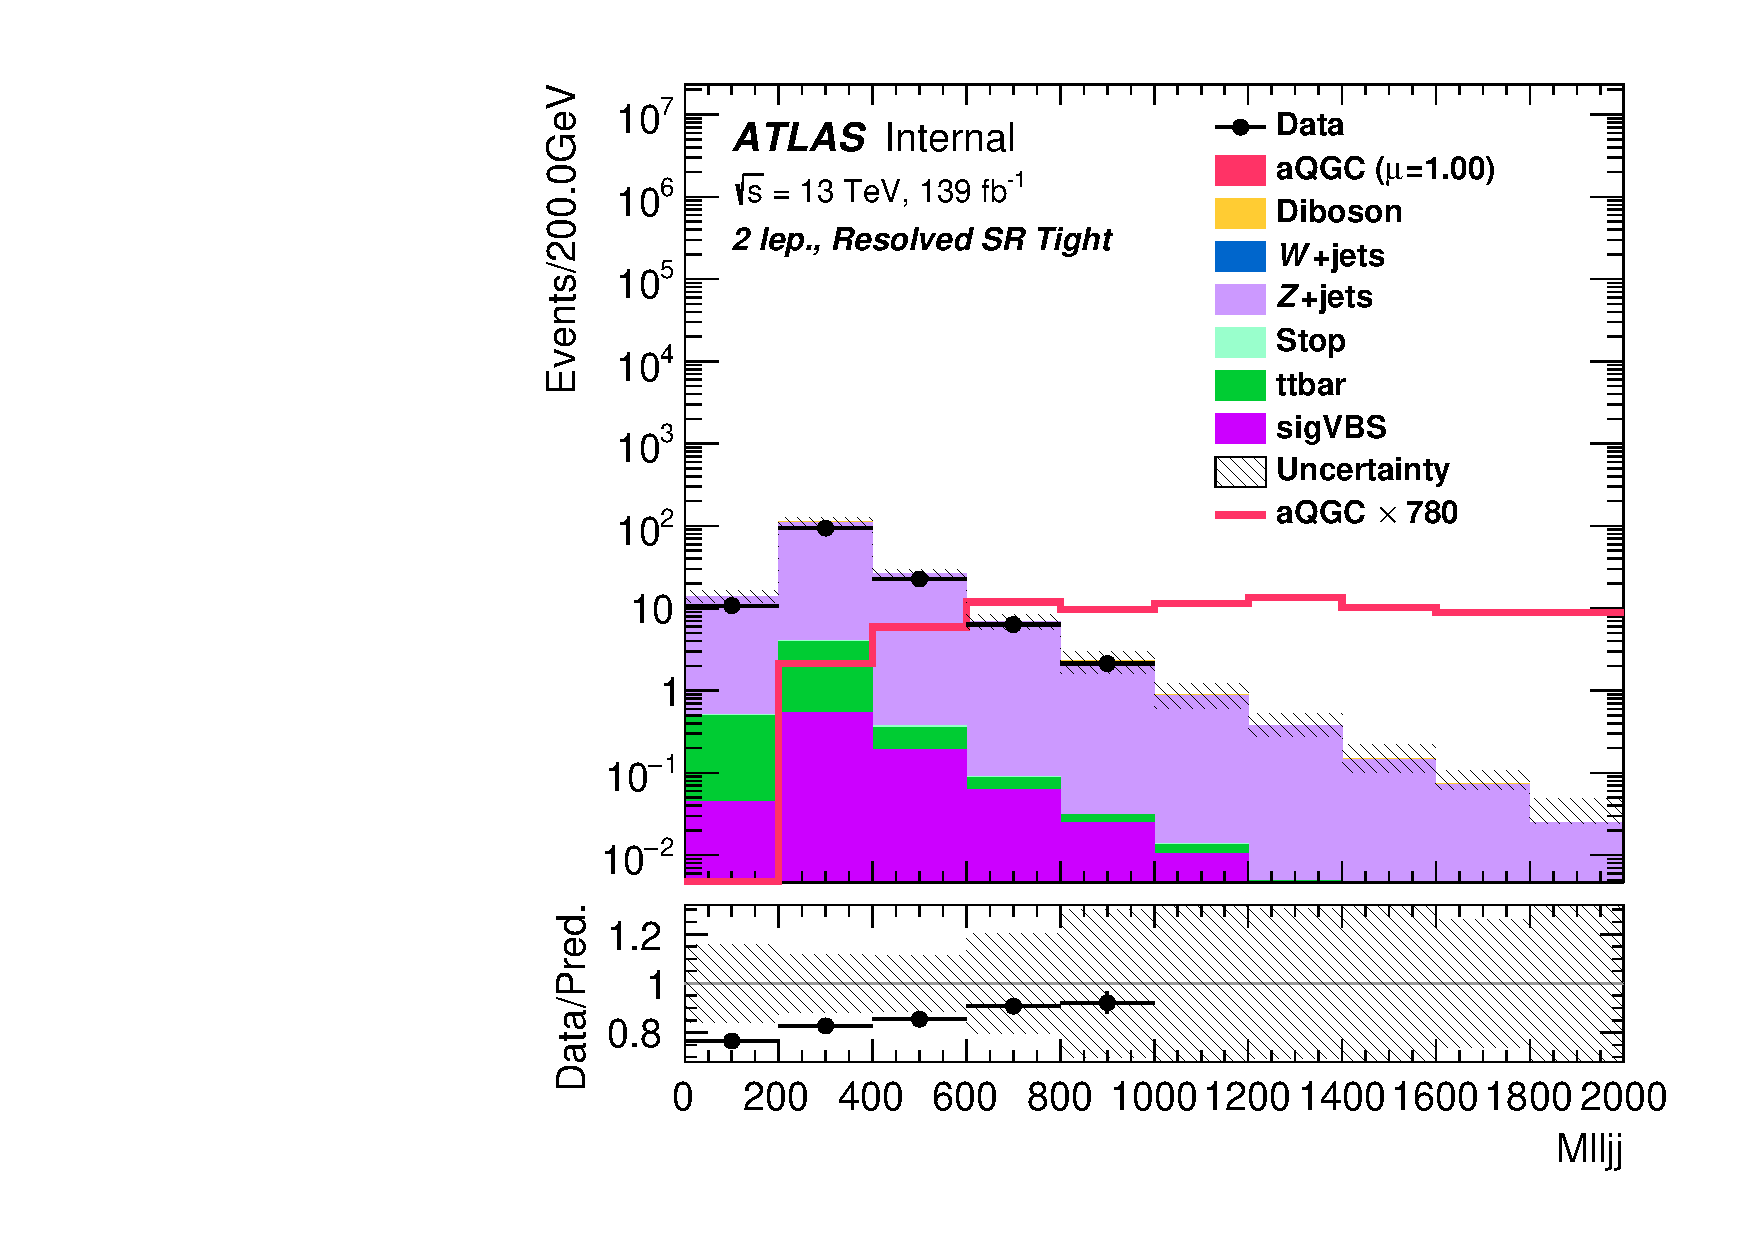
\includegraphics[width=0.32\textwidth]{figures/aQGC/MVV/Region_distMlljj_DSRVBSFid_BMin0_T0_Y6051_incTag1_J2_L2_incJet1_Prefitlog.pdf}
%    	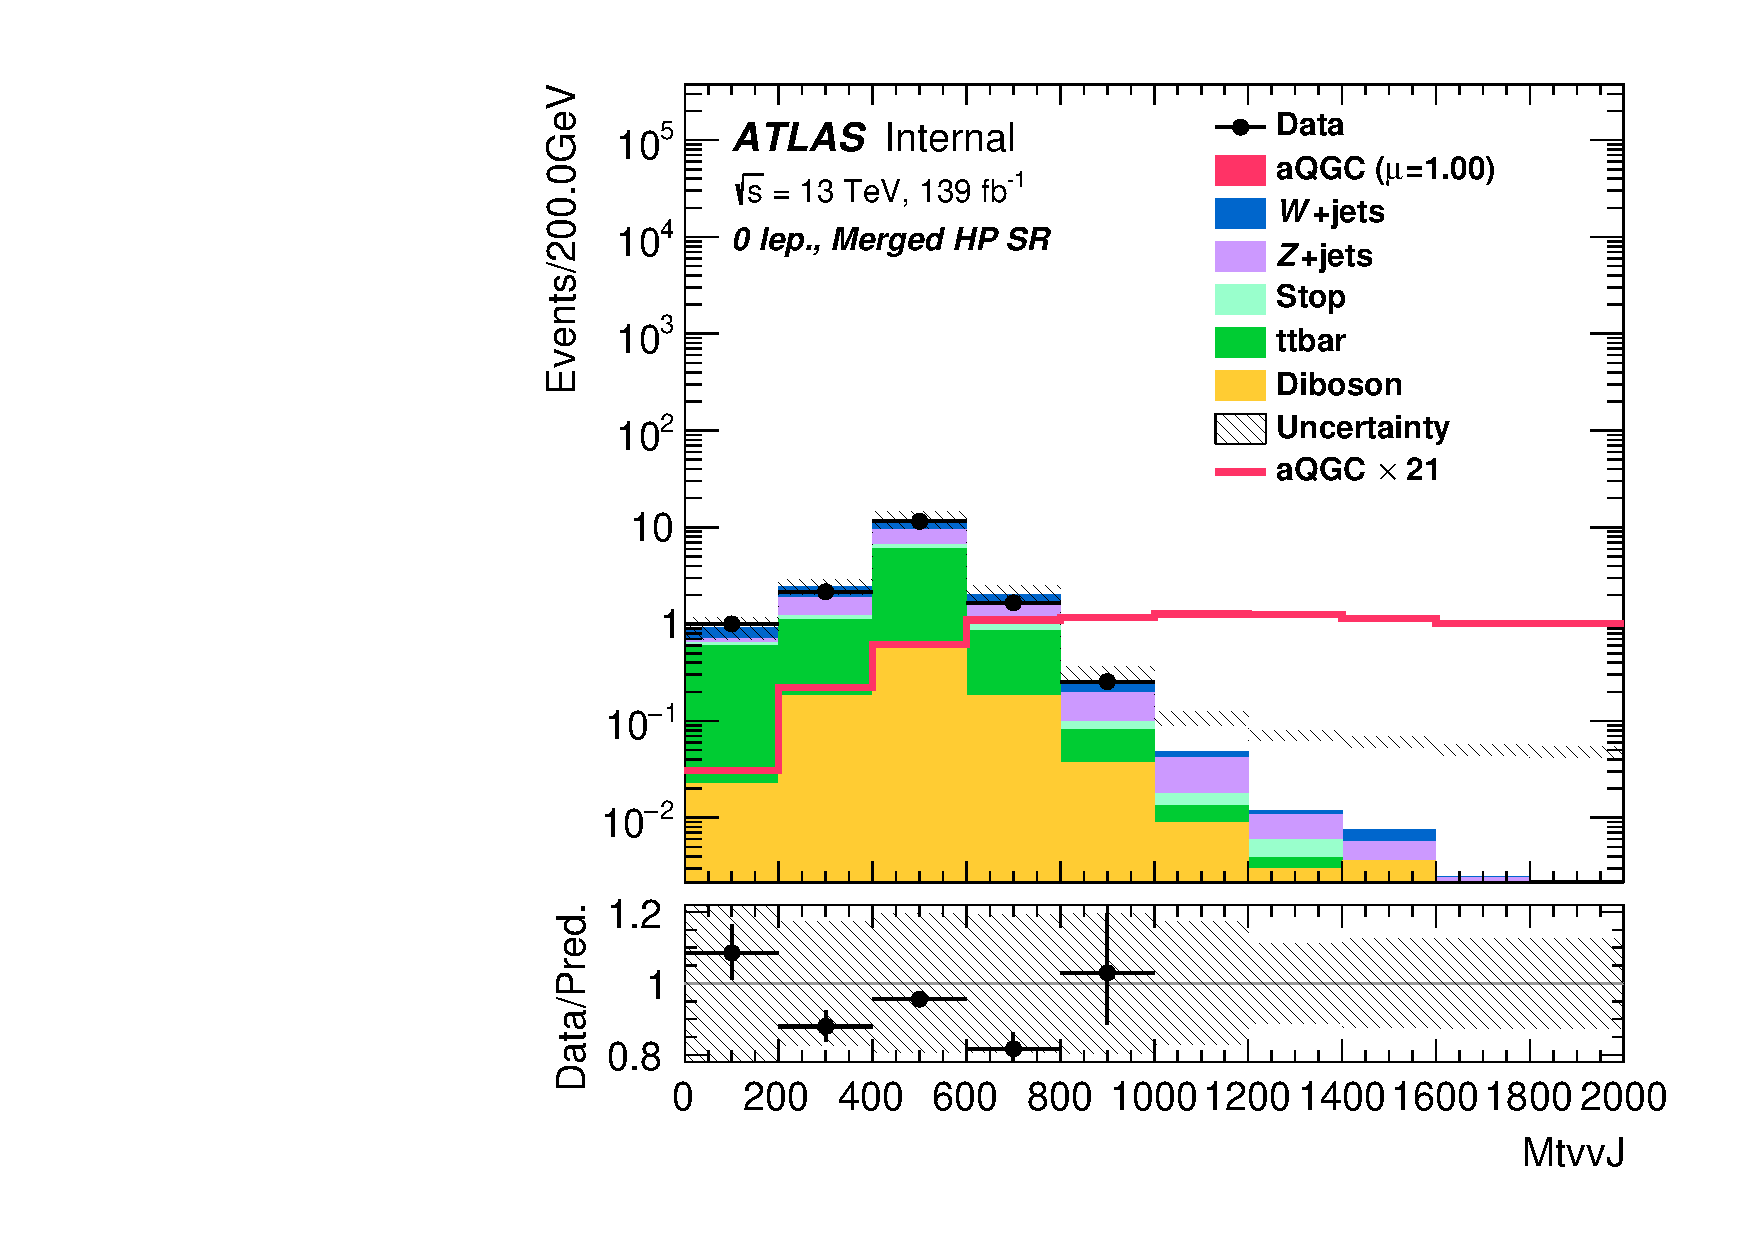
\includegraphics[width=0.32\textwidth]{figures/aQGC/MVV/Region_distMtvvJ_DSRVBSHP_BMin0_J0_incJet1_L0_T0_incFat1_Y6051_incTag1_Fat1_Prefitlog.pdf}
%    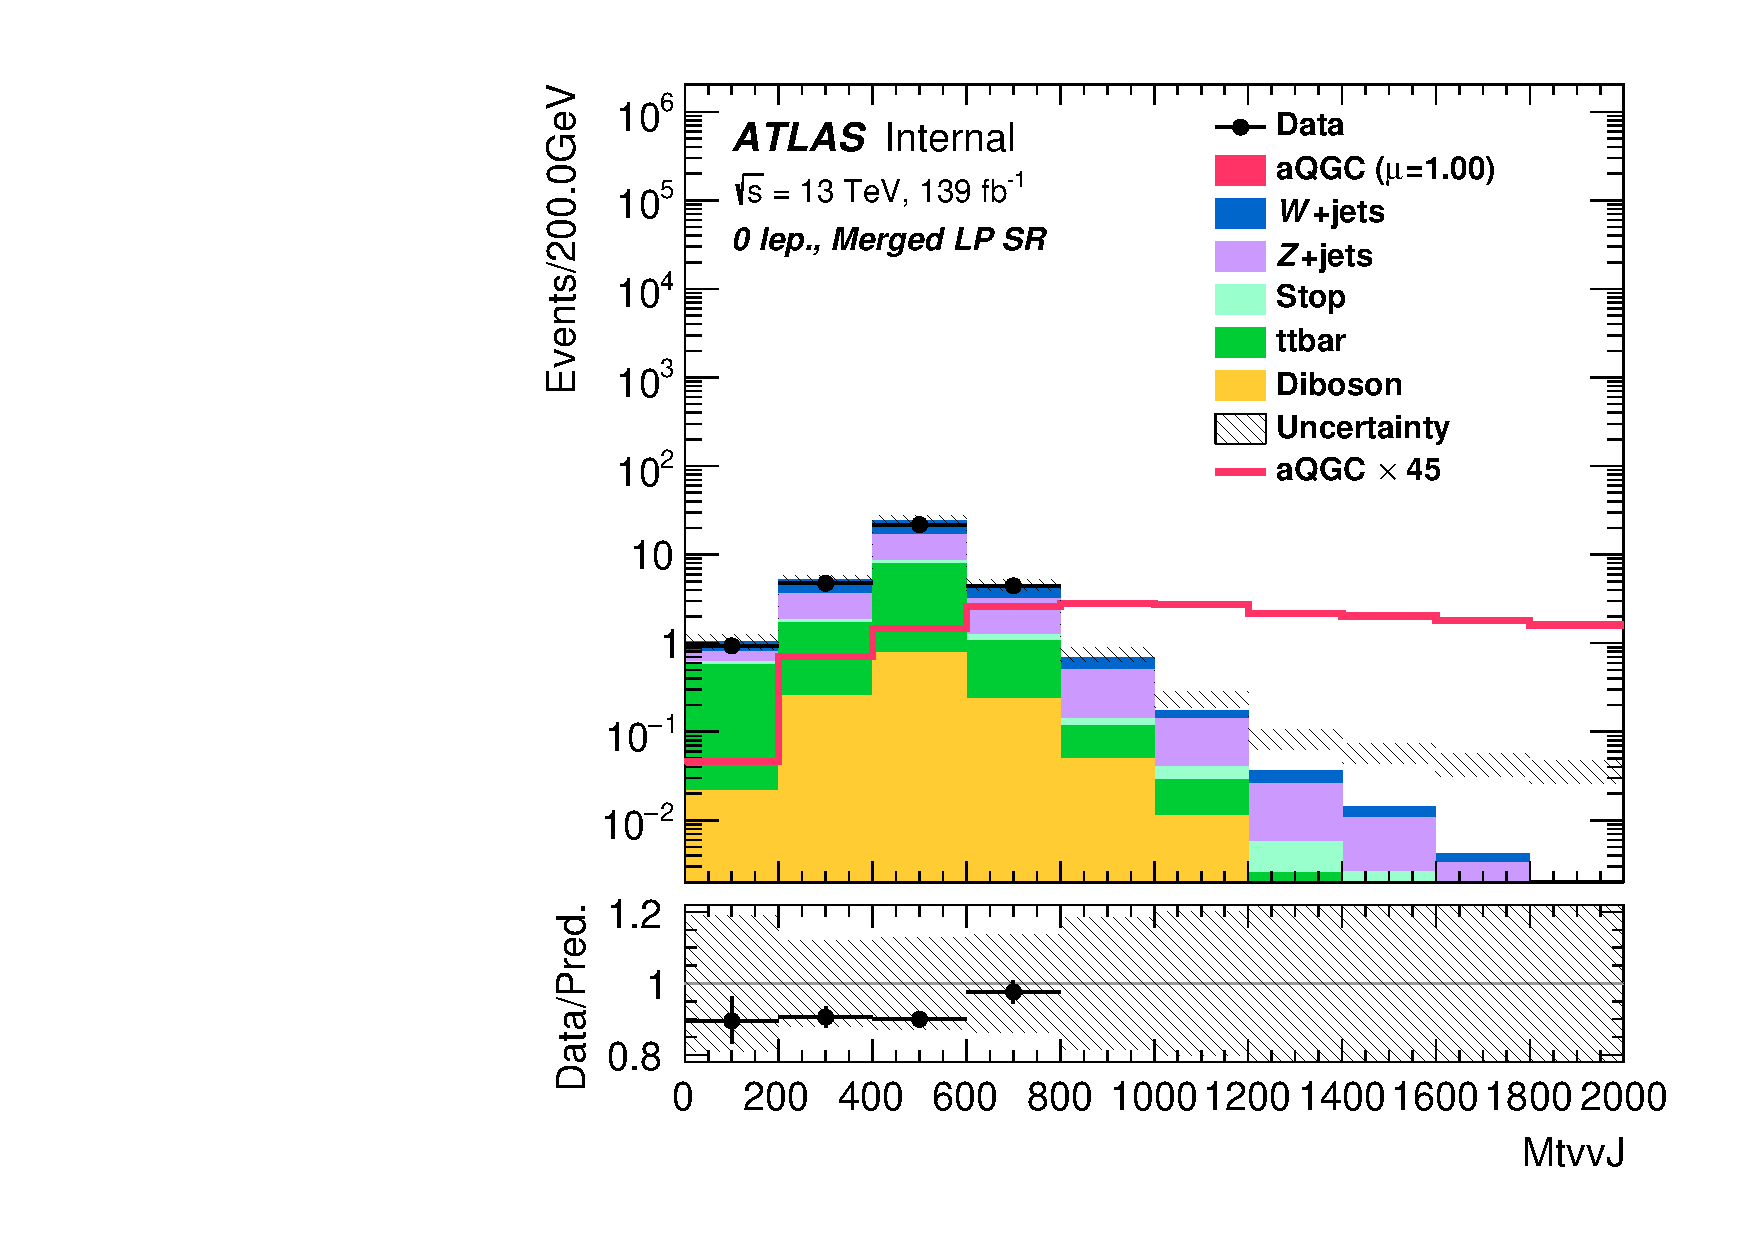
\includegraphics[width=0.32\textwidth]{figures/aQGC/MVV/Region_distMtvvJ_DSRVBSLP_BMin0_J0_incJet1_L0_T0_incFat1_Y6051_incTag1_Fat1_Prefitlog.pdf}
% 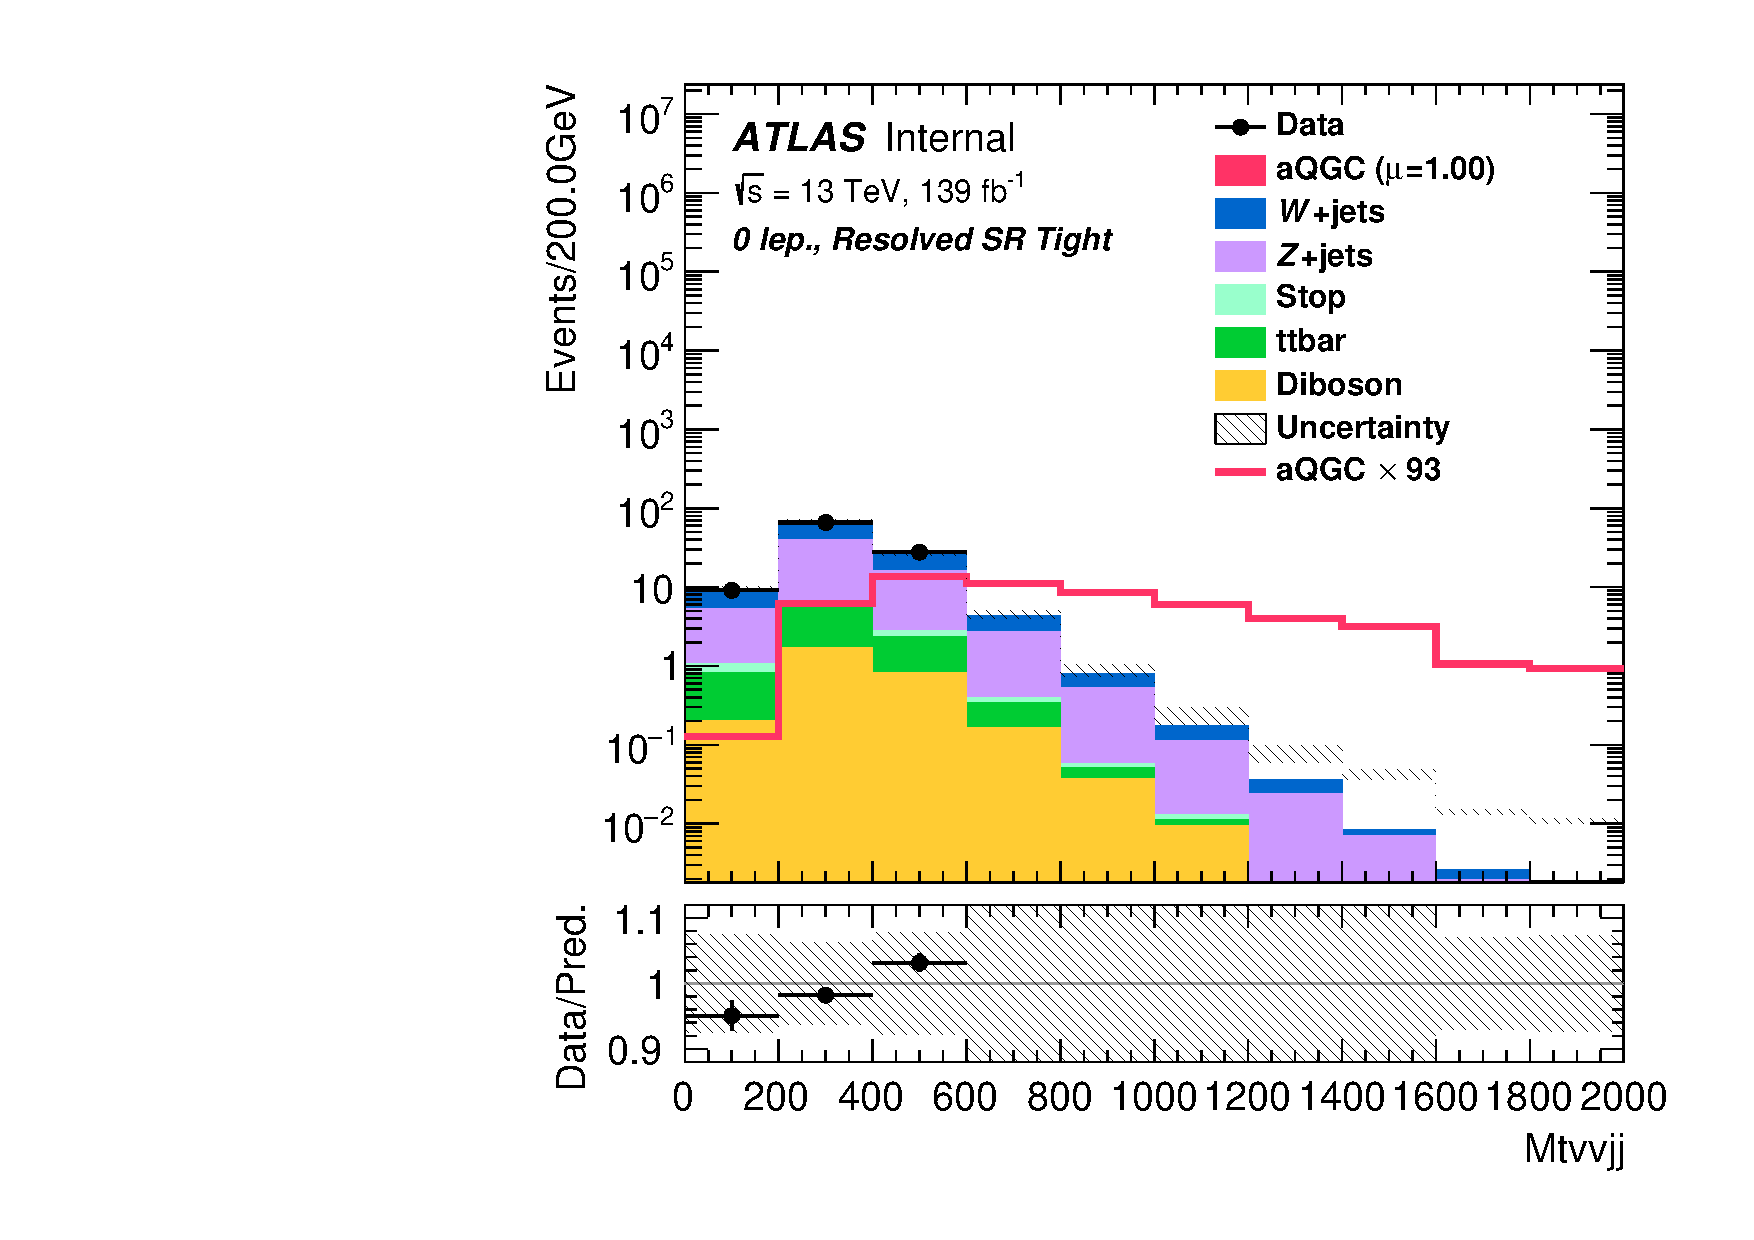
\includegraphics[width=0.32\textwidth]{figures/aQGC/MVV/Region_distMtvvjj_DSRVBSFid_BMin0_T0_Y6051_incTag1_J2_L0_incJet1_Prefitlog.pdf}
%        \caption{fig: $m_{VV}$ distribution for \tlep\ (left) and $m_{tv}$ distribution for \zlep\ (right)}
%        \label{fig:mVVdist}
%\end{figure}
\begin{table}[ht!]
\small
\begin{center}
%\resizebox{0.9\textwidth}{!}{
\begin{tabular}{ | l || l | l | l |}
\hline
Threshold values (GeV)          & SRVBS\_HP  & SRVBS\_LP & SRVBS\_Fid  \tabularnewline \hline
0-lepton & 1050      & 1200     & 1200       \tabularnewline \hline
1-lepton & 1500      & 1500     & 1500       \tabularnewline \hline
2-lepton & 1500      & 1500     & 1500       \tabularnewline \hline
\end{tabular}
\caption{Threshold value to separate the $m_{VV}$ distribution for the 1-lepton and the 2-lepton and $m_{tv}$ distribution for the 0-lepton channel. }
\label{tab:2binthreshold}
\end{center}
\end{table}

\section{Limits setting}
Finally, by using both quadratic and interference terms as a combined signal template, the expected 95\% CL upper and lower limits are obtained by the fit to the Asimov dataset constructed from the background plus SM EW VV+jj samples, as well as observed limits with data.
All SRs in \zlep, \olep\, and \tlep\ channels are separated into low- and high-$m_{VV}$ bins as discussed in Section~\ref{subsec:2binapproach} and combined statistically.
All systematic uncertainties discussed for Standard Model measurement are included in the fitting.
The SM EW VV+jj signal samples are added to the background as a free floated normalization factor, and all the analysis regions are correlated with EW VV+jj signal samples.
Due to the small statistics in high-$m_{VV}$ regions compared with the low-$m_{VV}$ regions, the overall behaviors of the post-fit nuisance parameters are almost the same as the SM measurement.
The postfit plots for FT0 parameter in signal regions are shown in figure~\ref{fig:postSR0lepaQGC}, \ref{fig:postSR1lepaQGC},\ref{fig:postSR2lepaQGC}. 
Overall the expected background reproduces the data well within the uncertainty except for the several right-most bins of the high-$m_{VV}$ region.
In the right-most bins of the high-$m_{VV}$ region, some data excess can be seen in the 0-lepton resolved signal region and in the 1-lepton merged LP signal region.
\begin{figure}[]
    \centering
    %0lep
    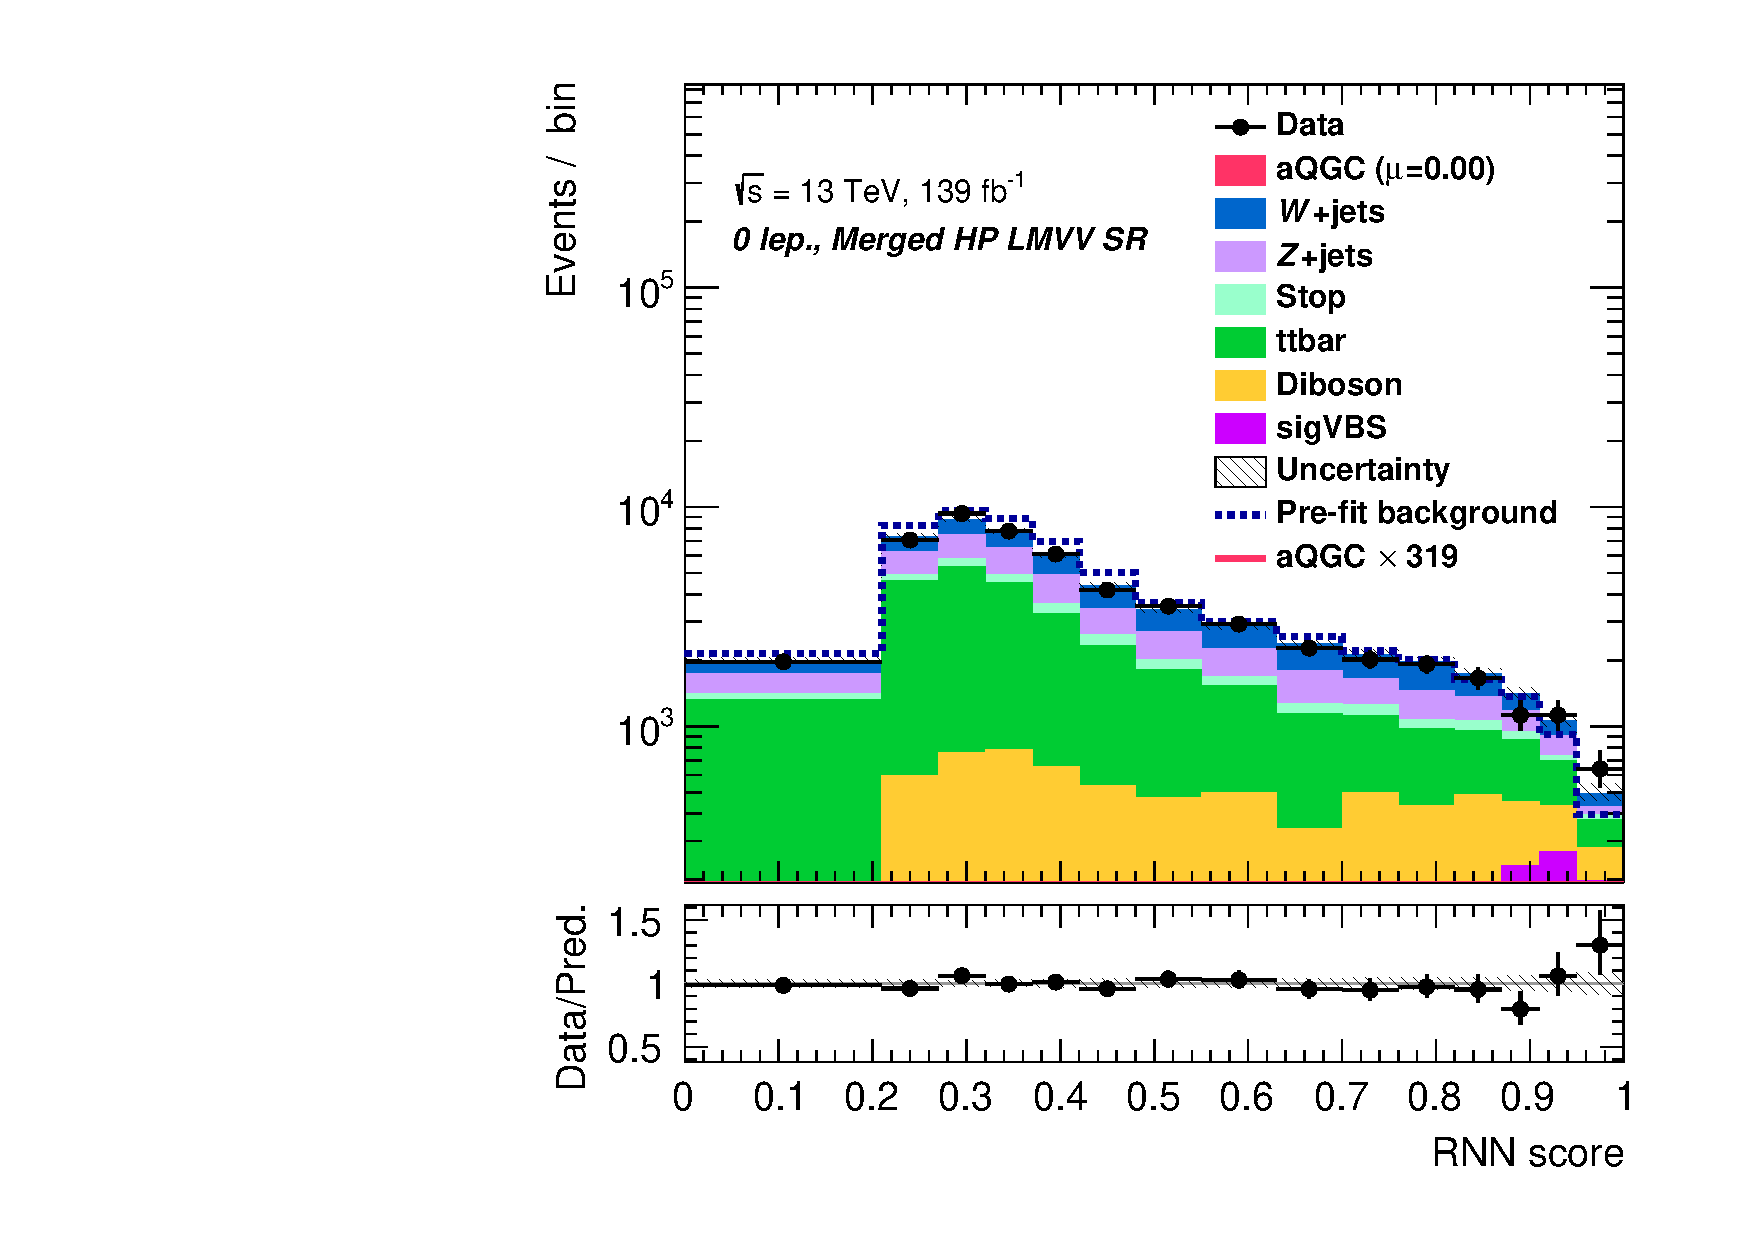
\includegraphics[width=0.45\textwidth]{figures/aQGC/PostFit/Region_distRNN_DSRVBSHPLMtvvJ1050_BMin0_J0_incJet1_L0_T0_incFat1_Y6051_incTag1_Fat1_GlobalFit_unconditionnal_mu1log}
    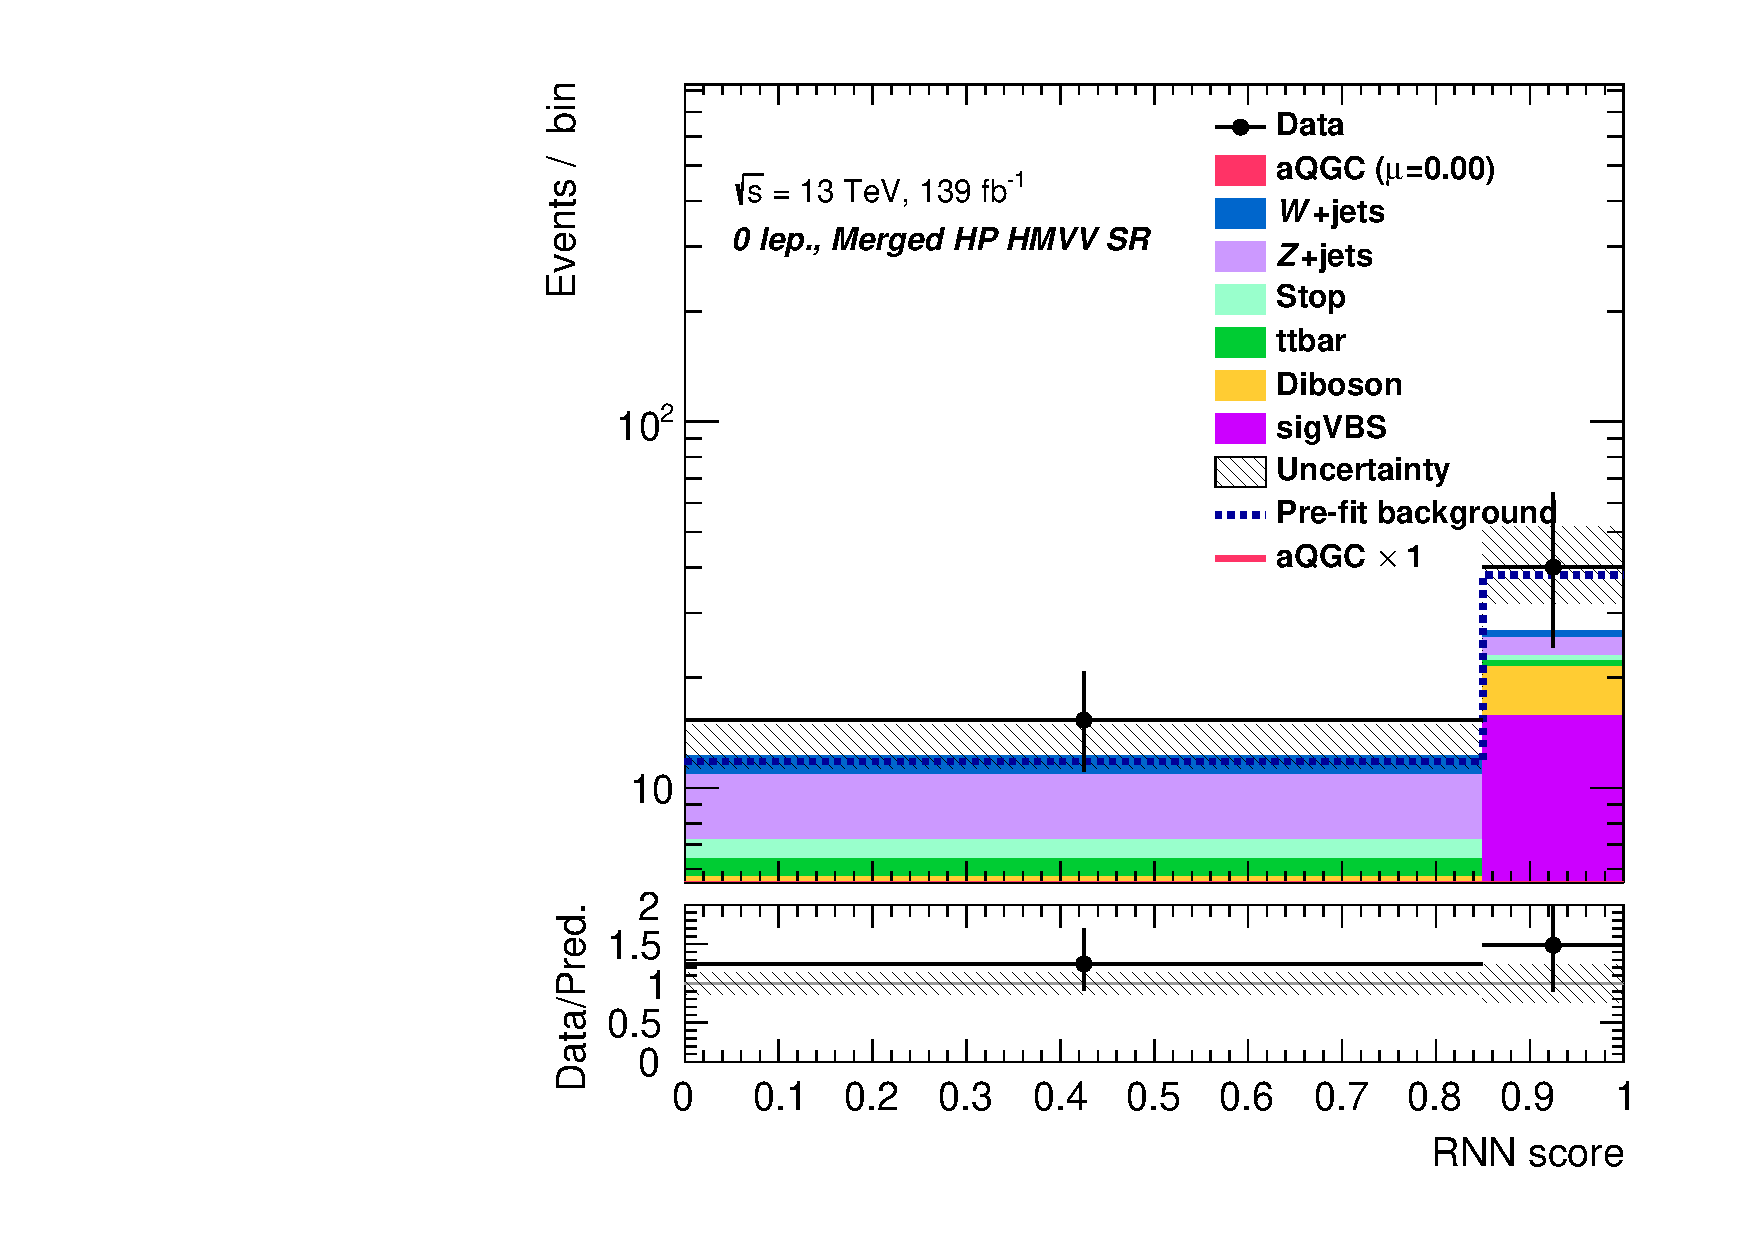
\includegraphics[width=0.45\textwidth]{figures/aQGC/PostFit/Region_distRNN_DSRVBSHPHMtvvJ1050_BMin0_J0_incJet1_L0_T0_incFat1_Y6051_incTag1_Fat1_GlobalFit_unconditionnal_mu1log}    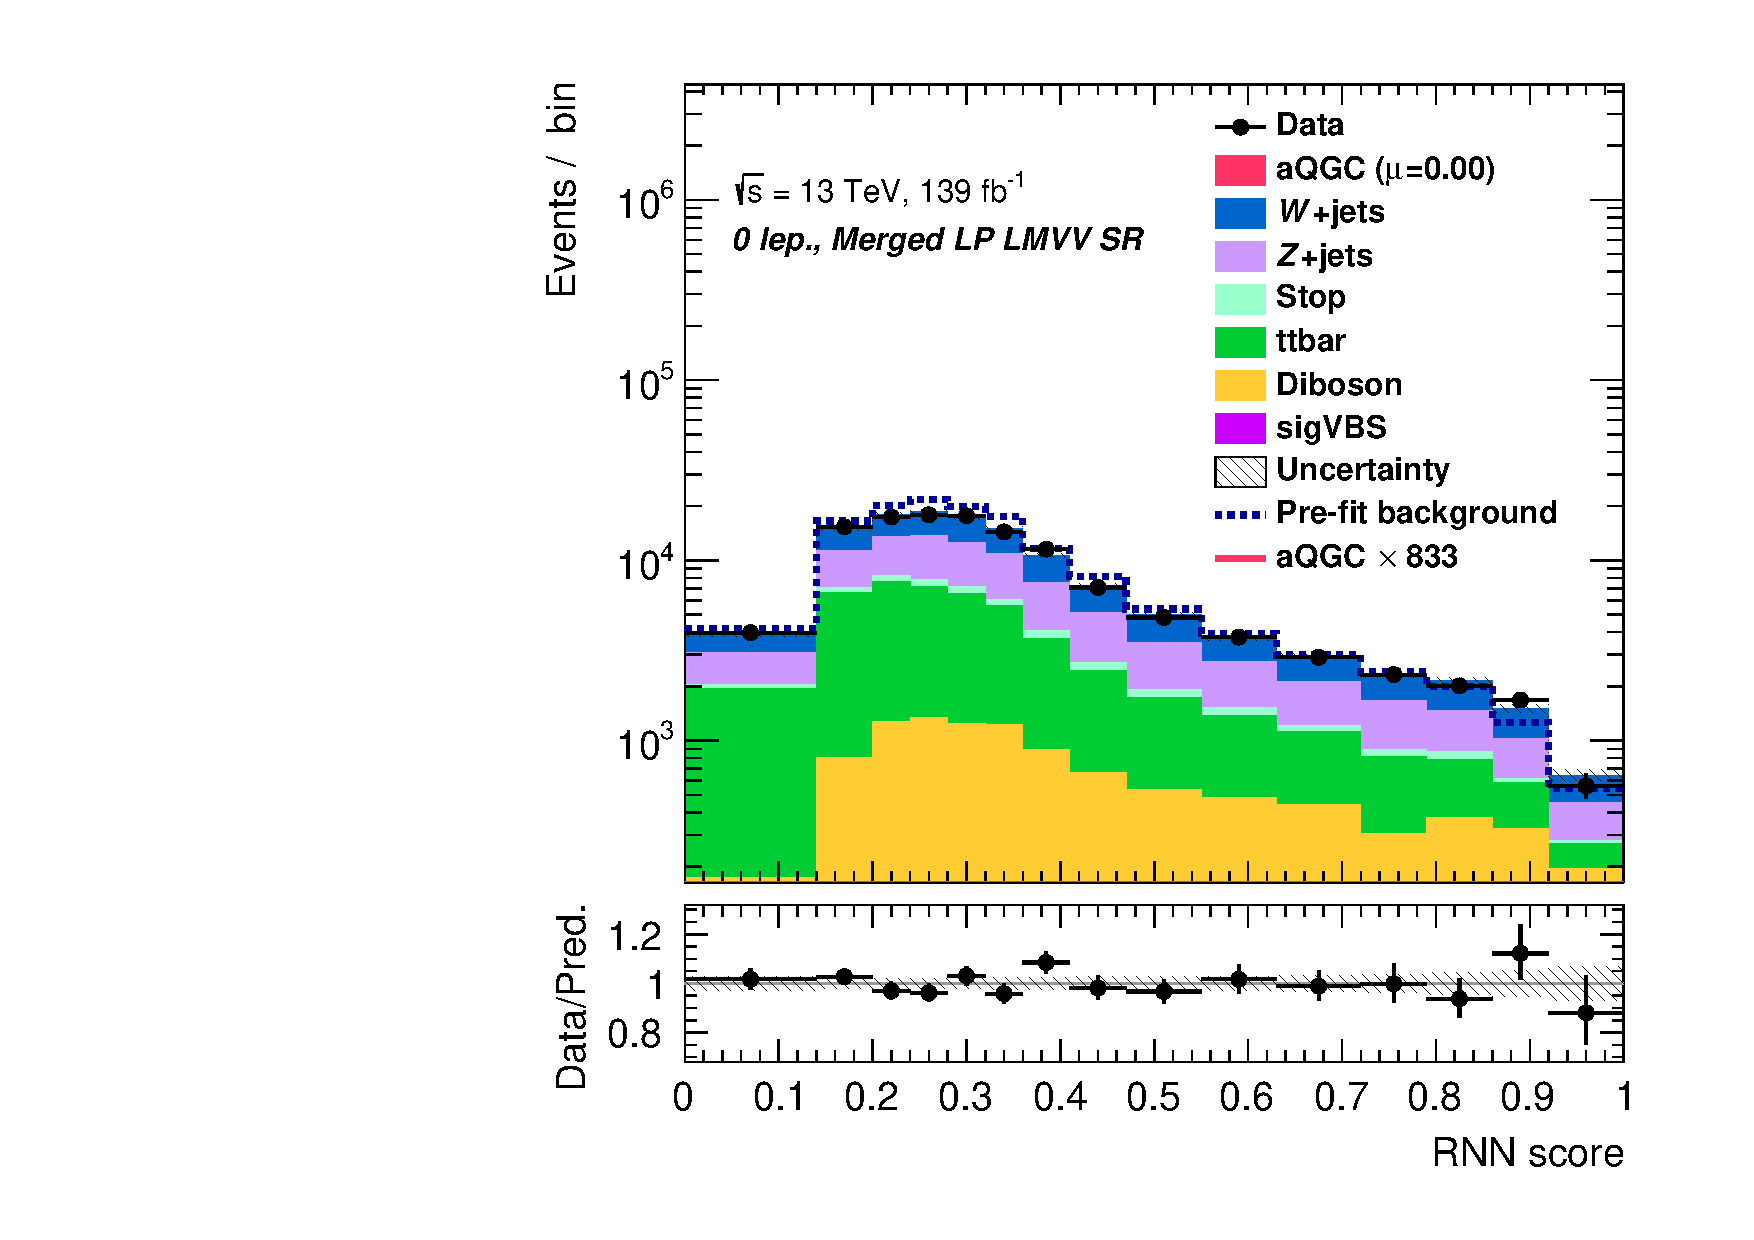
\includegraphics[width=0.45\textwidth]{figures/aQGC/PostFit/Region_distRNN_DSRVBSLPLMtvvJ1200_BMin0_J0_incJet1_L0_T0_incFat1_Y6051_incTag1_Fat1_GlobalFit_unconditionnal_mu1log}     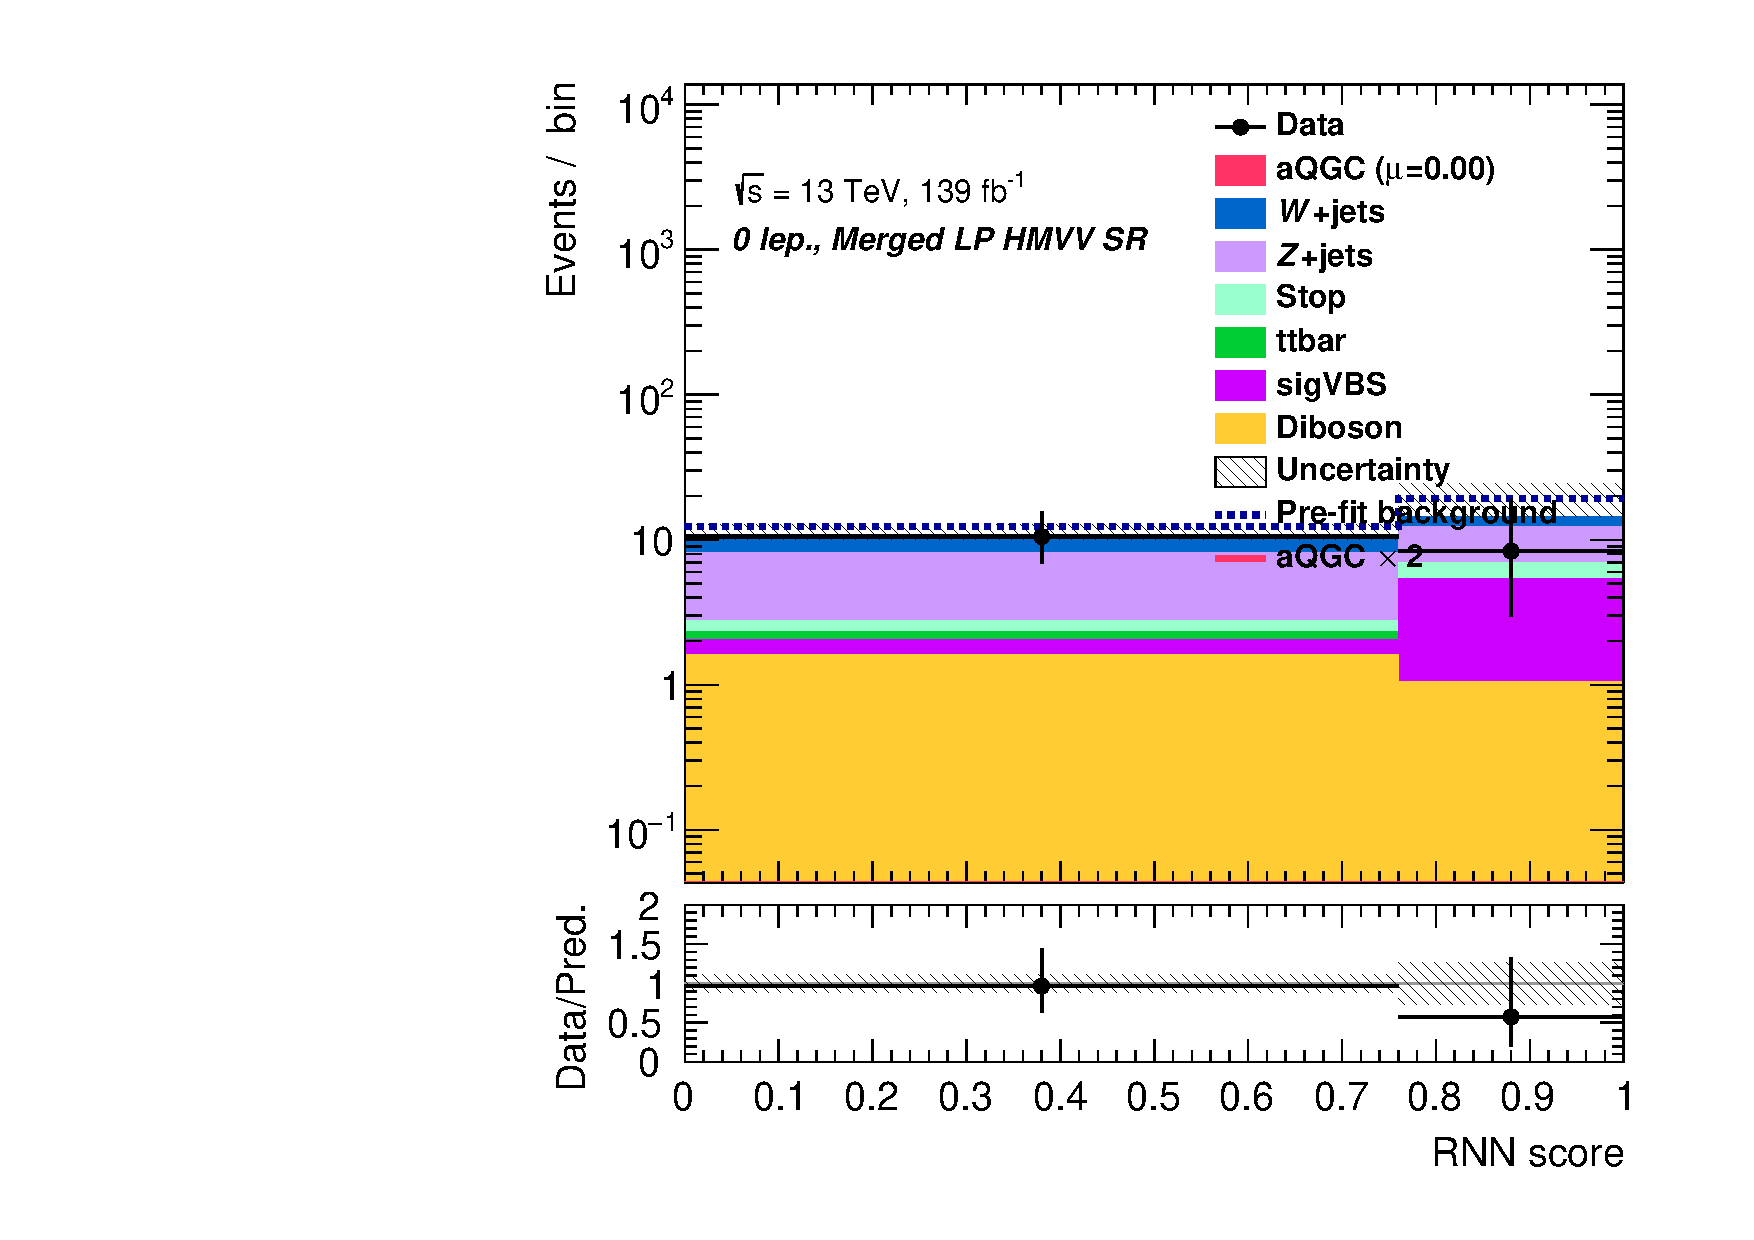
\includegraphics[width=0.45\textwidth]{figures/aQGC/PostFit/Region_distRNN_DSRVBSLPHMtvvJ1200_BMin0_J0_incJet1_L0_T0_incFat1_Y6051_incTag1_Fat1_GlobalFit_unconditionnal_mu1log}    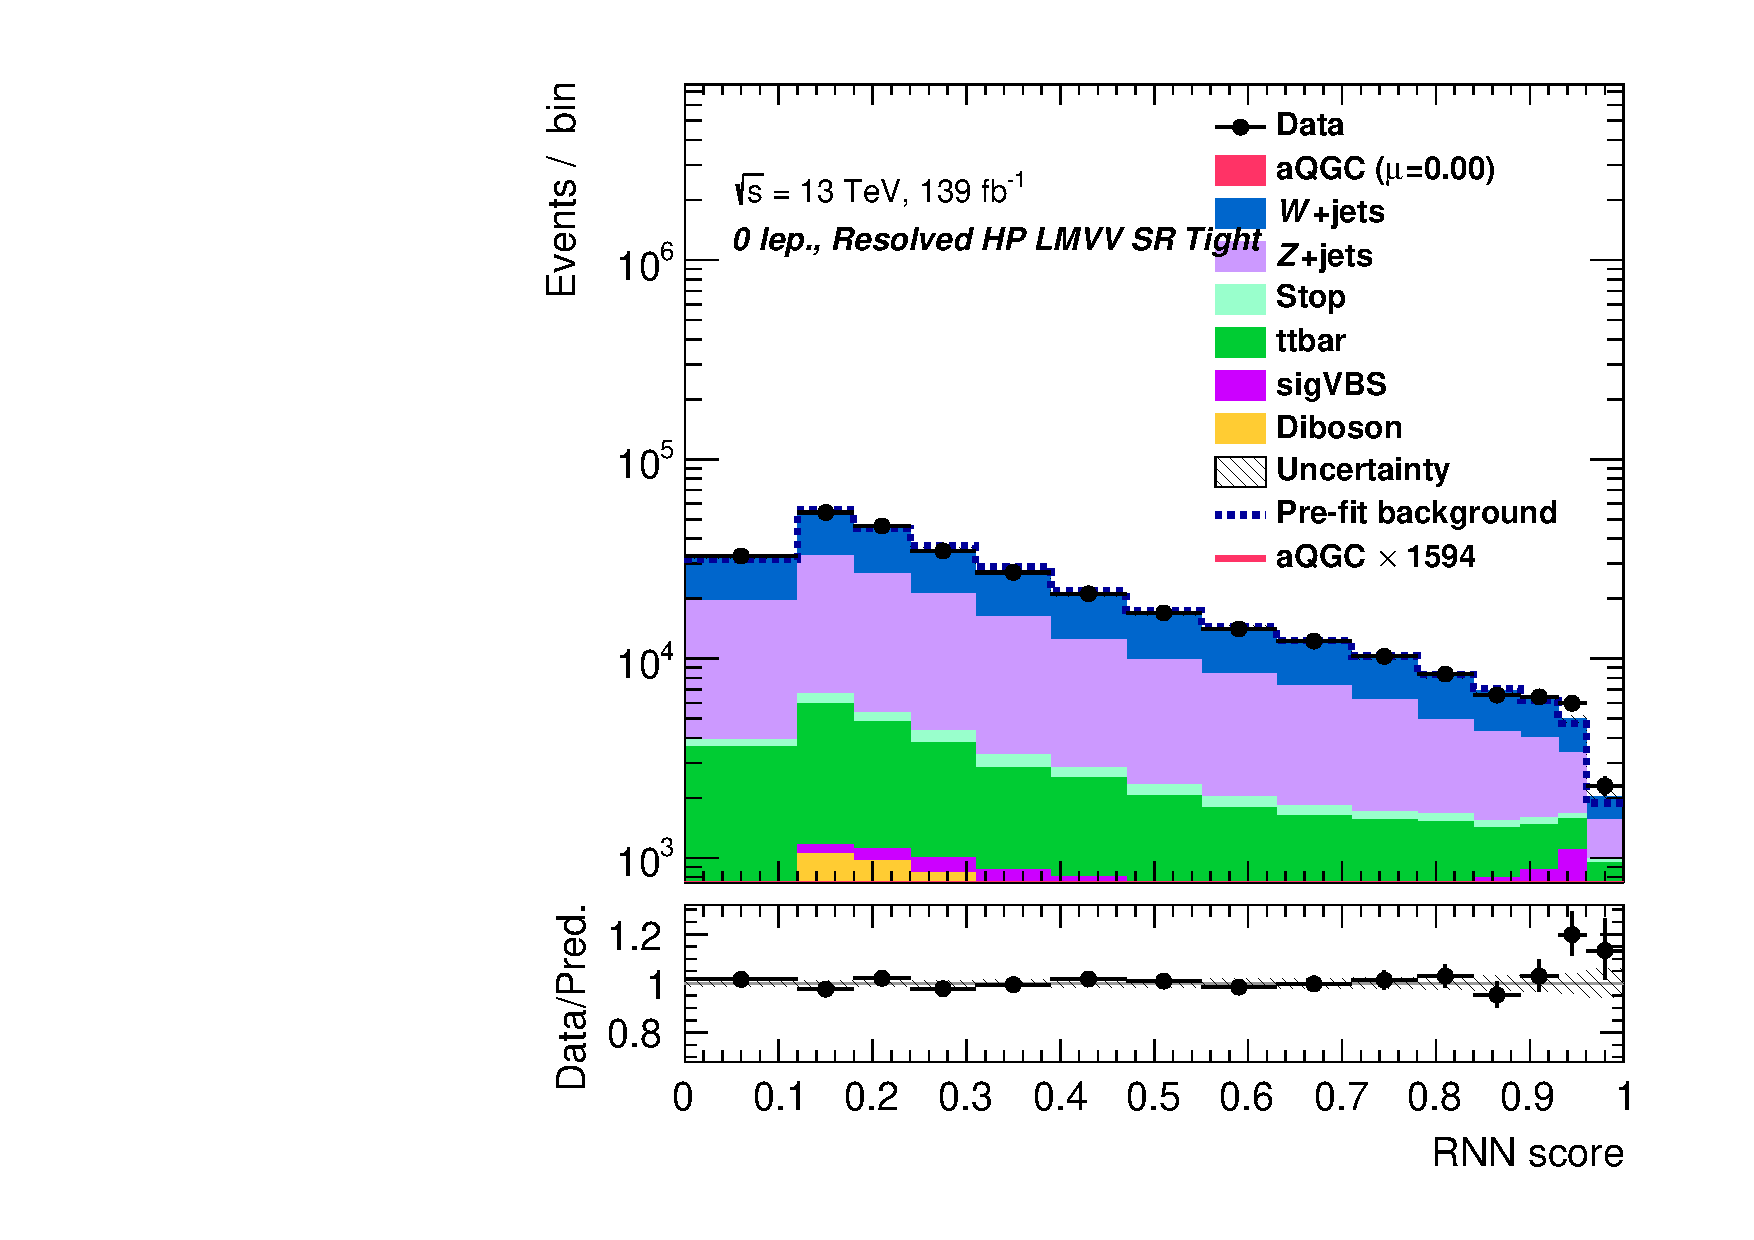
\includegraphics[width=0.45\textwidth]{figures/aQGC/PostFit/Region_distRNN_DSRVBSFidLMtvvjj1200_BMin0_T0_Y6051_incTag1_J2_L0_incJet1_GlobalFit_unconditionnal_mu1log}
    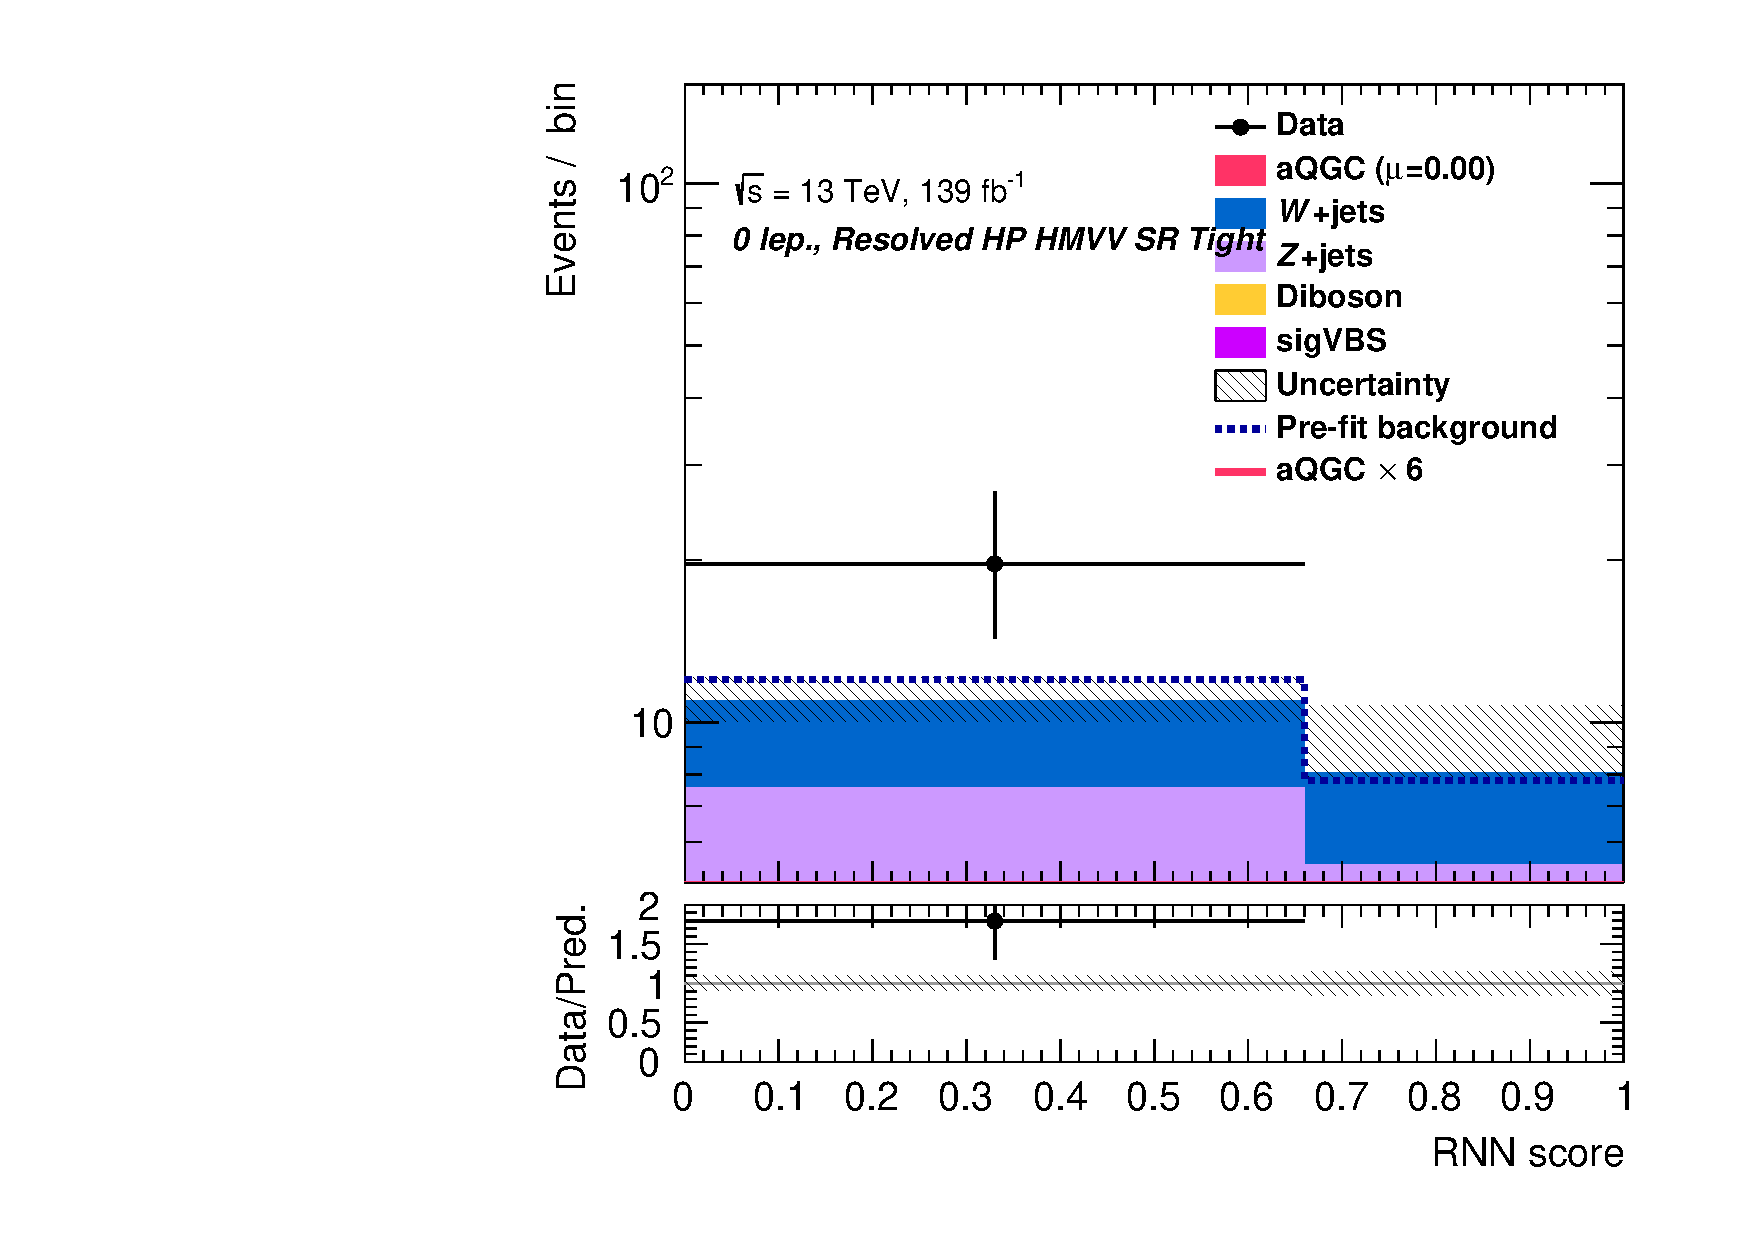
\includegraphics[width=0.45\textwidth]{figures/aQGC/PostFit/Region_distRNN_DSRVBSFidHMtvvjj1200_BMin0_T0_Y6051_incTag1_J2_L0_incJet1_GlobalFit_unconditionnal_mu1log}
      \caption{Comparisons of the observed data and expected background distributions of RNN score in 0-lepton channel signal regions. Low-$m_{VV}$ region (left) and the high-$m_{VV}$ region (right) are shown.}
      \label{fig:postSR0lepaQGC}
\end{figure}
\begin{figure}[]
    \centering
    %1lep
    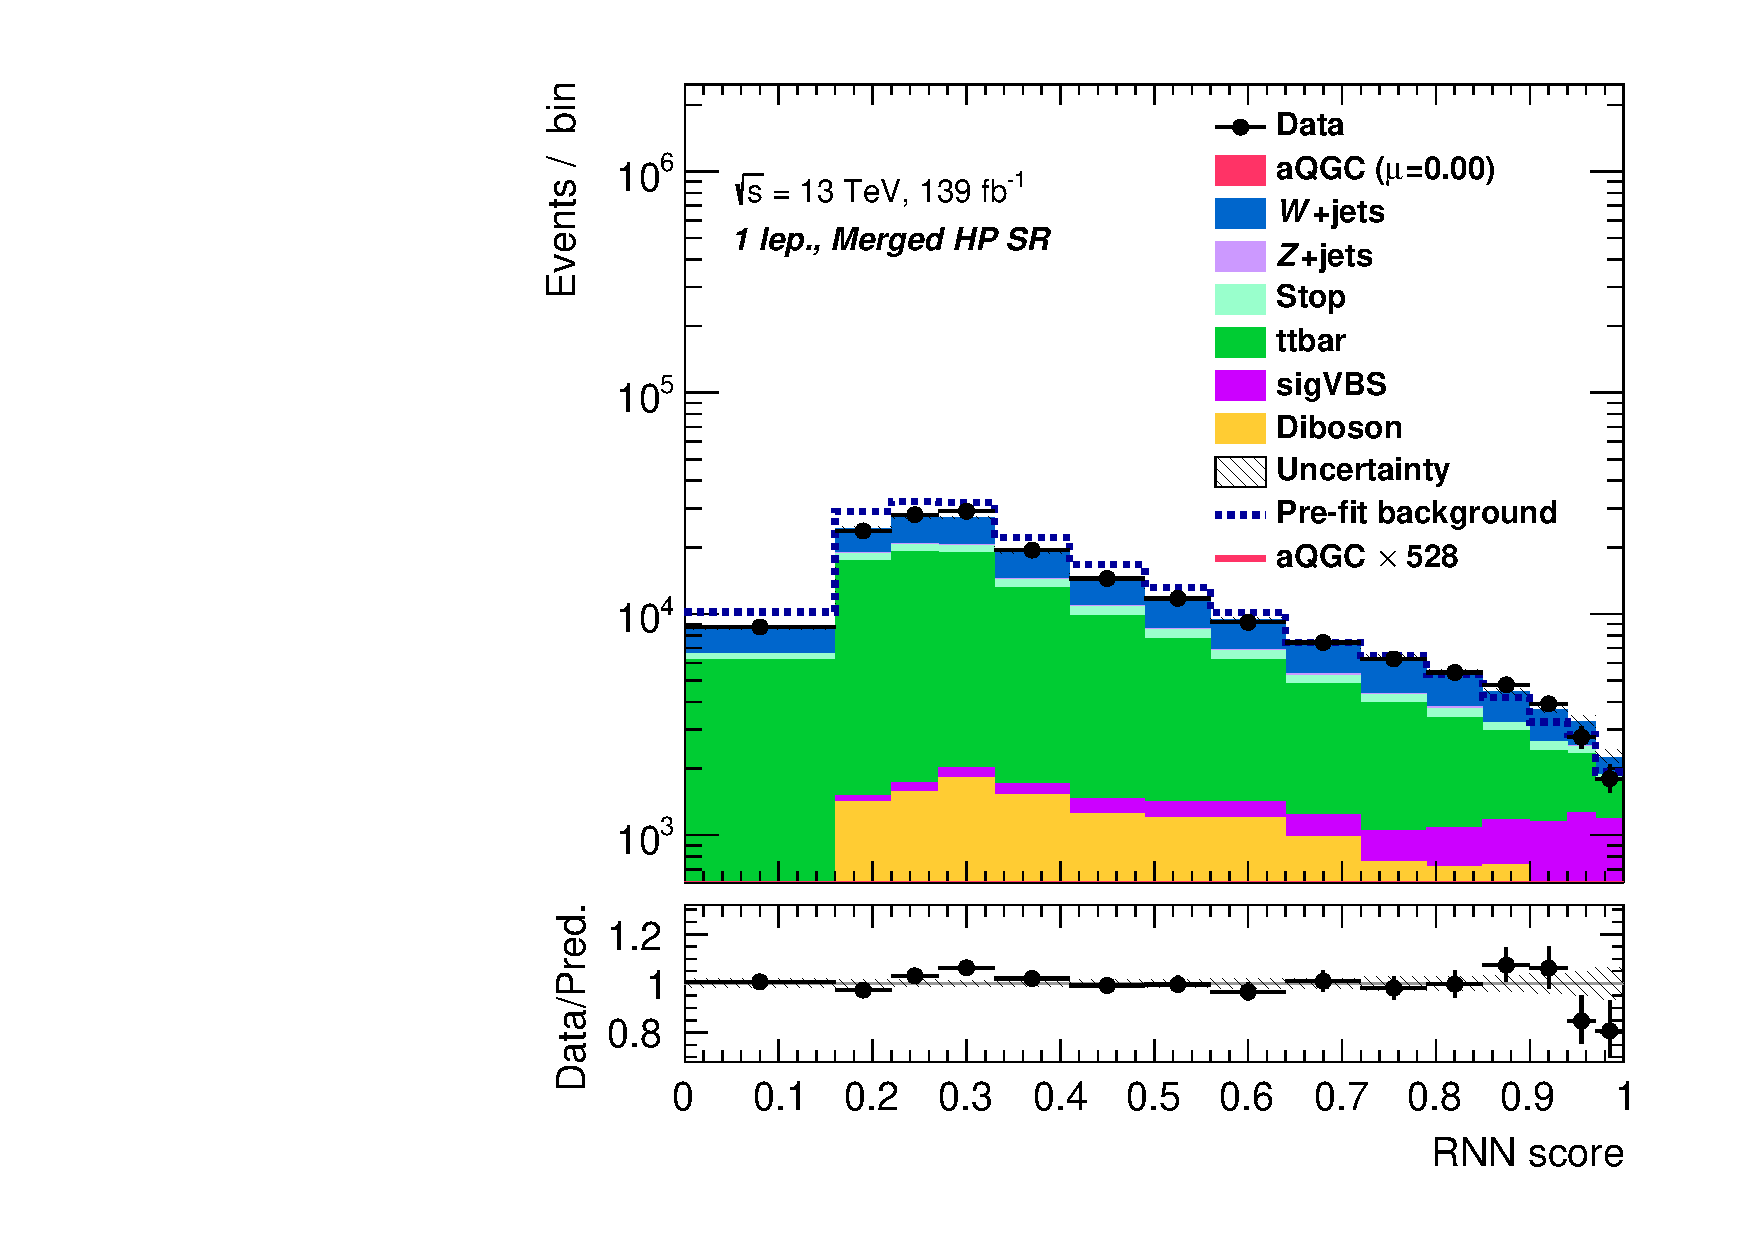
\includegraphics[width=0.45\textwidth]{figures/aQGC/PostFit/Region_distRNN_DSRVBSHPLMlvJ1500_BMin0_J0_incJet1_L1_T0_incFat1_Y6051_incTag1_Fat1_GlobalFit_unconditionnal_mu1log}
    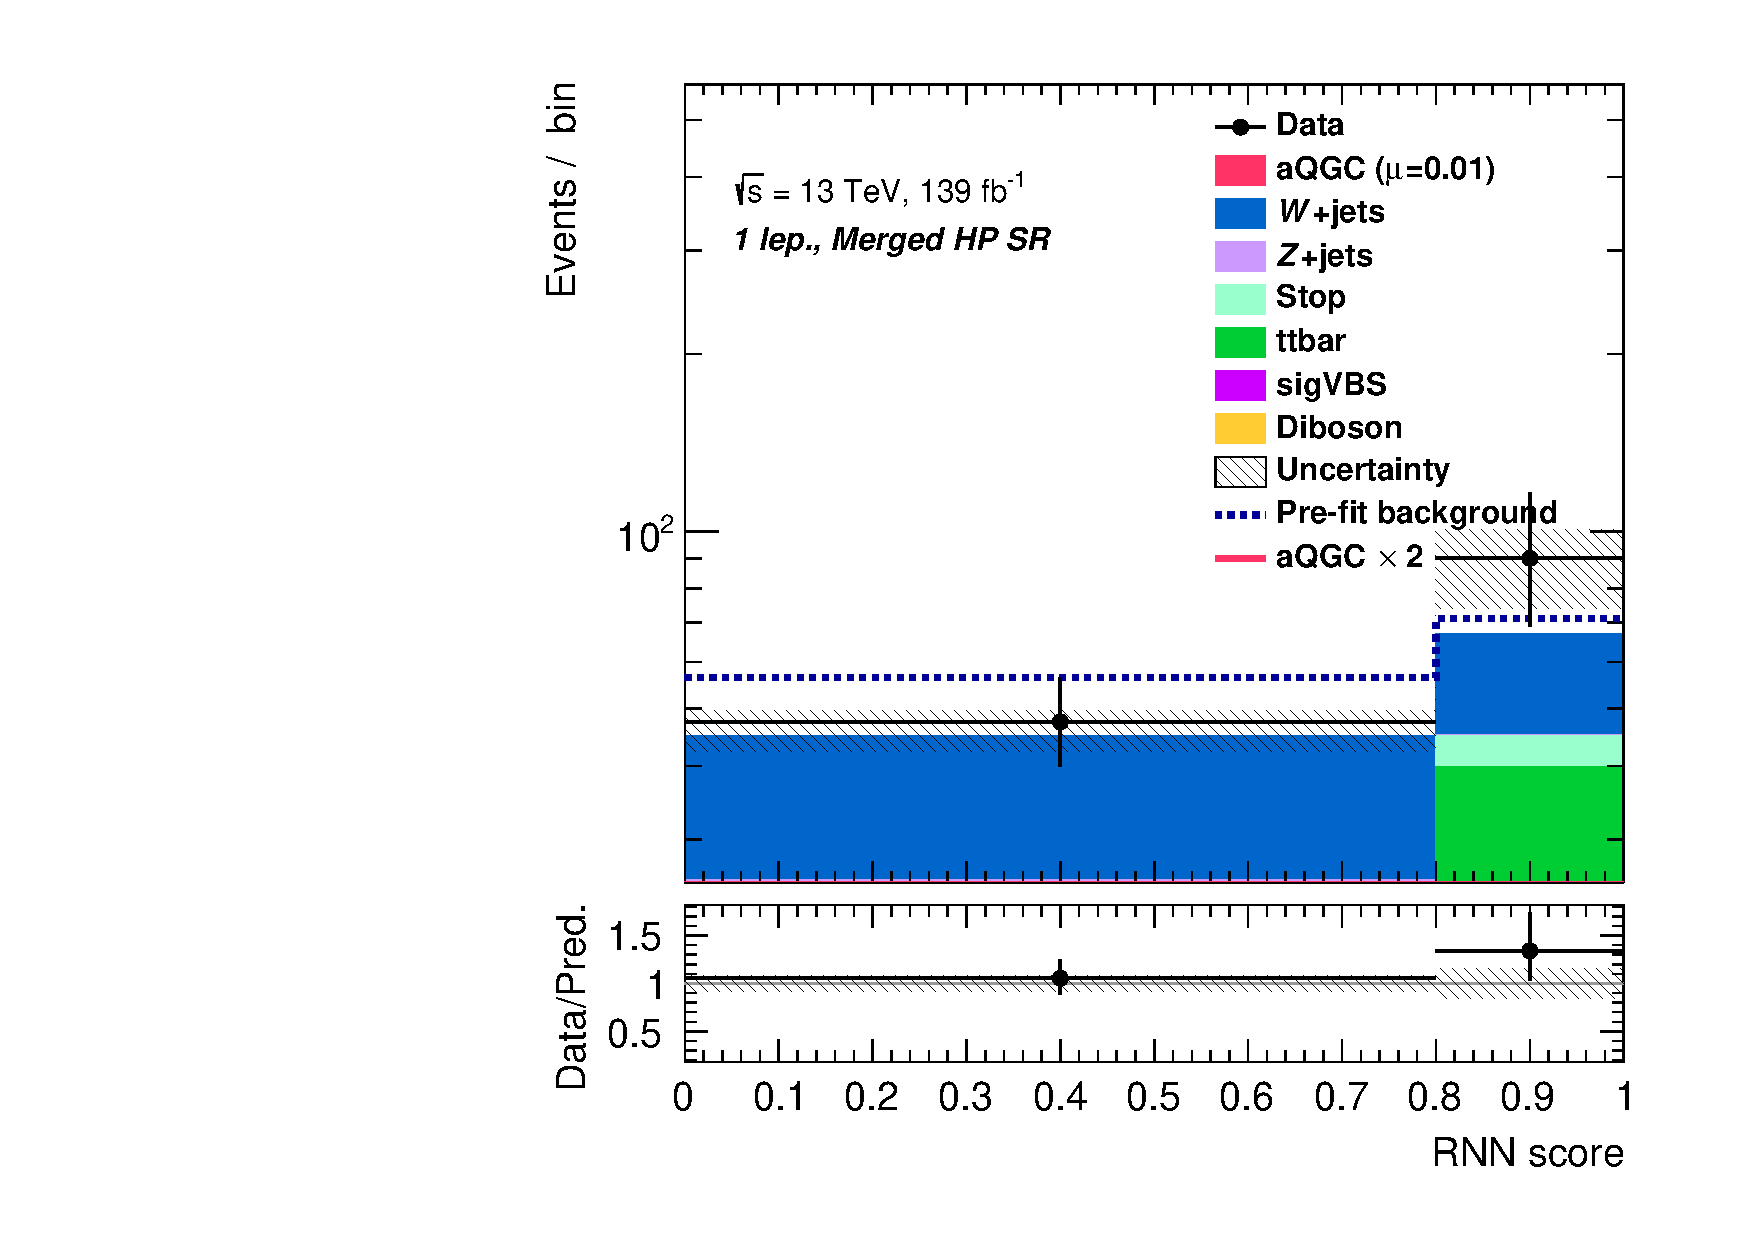
\includegraphics[width=0.45\textwidth]{figures/aQGC/PostFit/Region_distRNN_DSRVBSHPHMlvJ1500_BMin0_J0_incJet1_L1_T0_incFat1_Y6051_incTag1_Fat1_GlobalFit_unconditionnal_mu1log}
    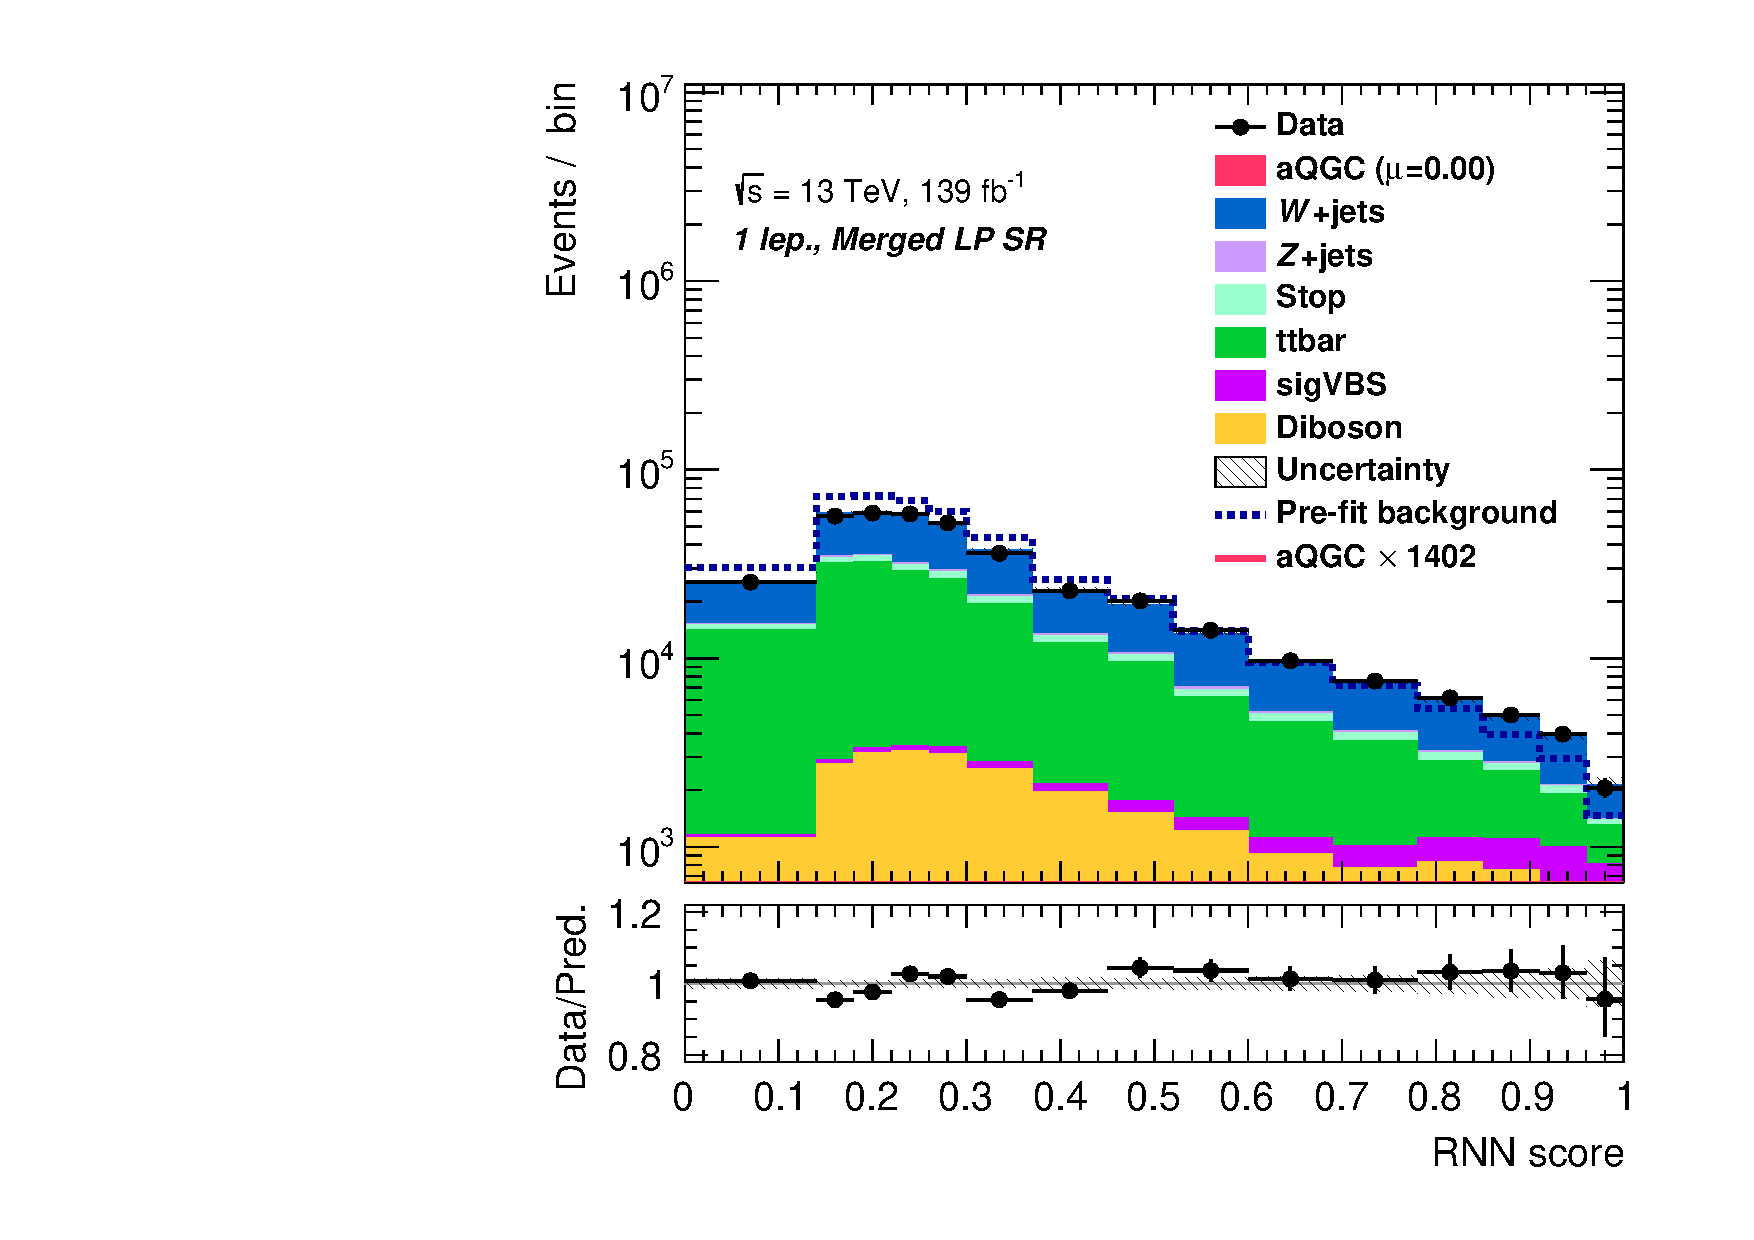
\includegraphics[width=0.45\textwidth]{figures/aQGC/PostFit/Region_distRNN_DSRVBSLPLMlvJ1500_BMin0_J0_incJet1_L1_T0_incFat1_Y6051_incTag1_Fat1_GlobalFit_unconditionnal_mu1log}
    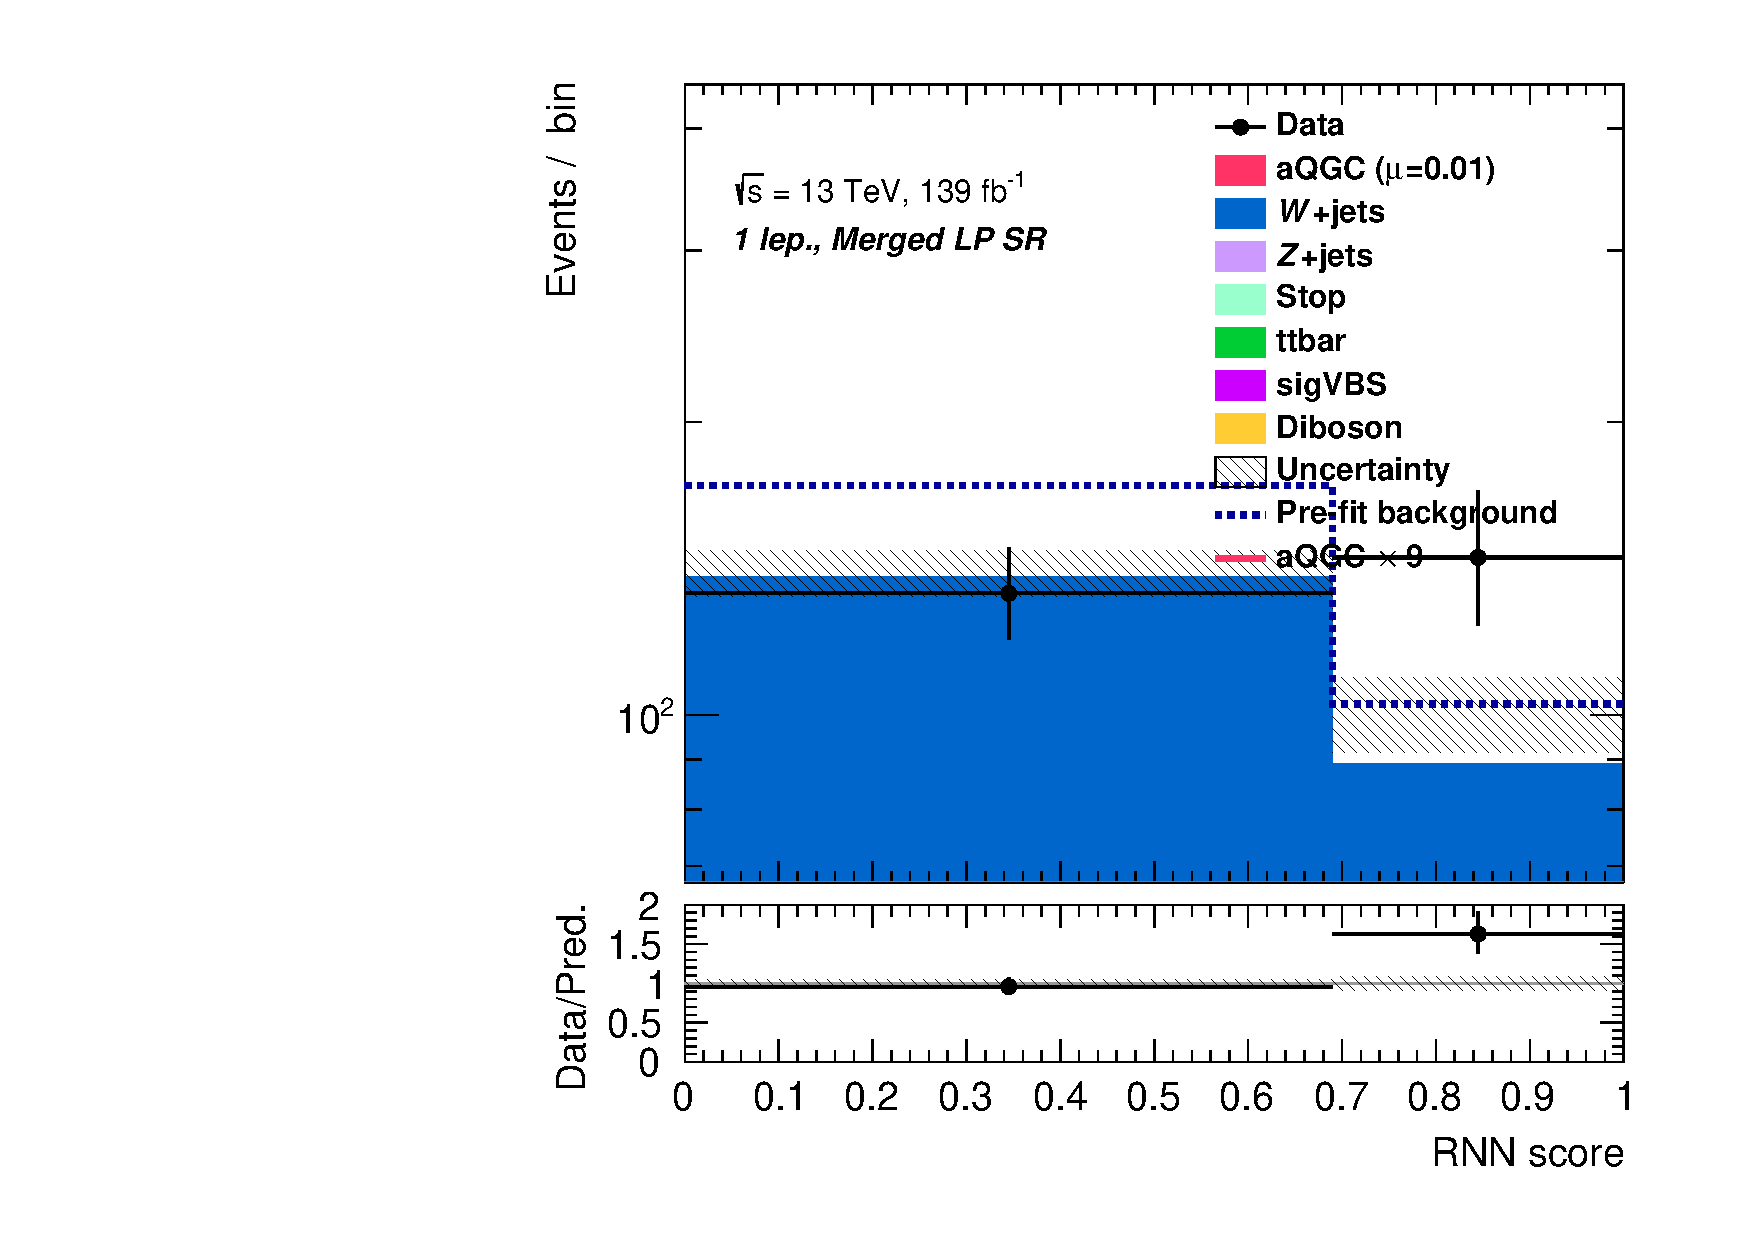
\includegraphics[width=0.45\textwidth]{figures/aQGC/PostFit/Region_distRNN_DSRVBSLPHMlvJ1500_BMin0_J0_incJet1_L1_T0_incFat1_Y6051_incTag1_Fat1_GlobalFit_unconditionnal_mu1log}
    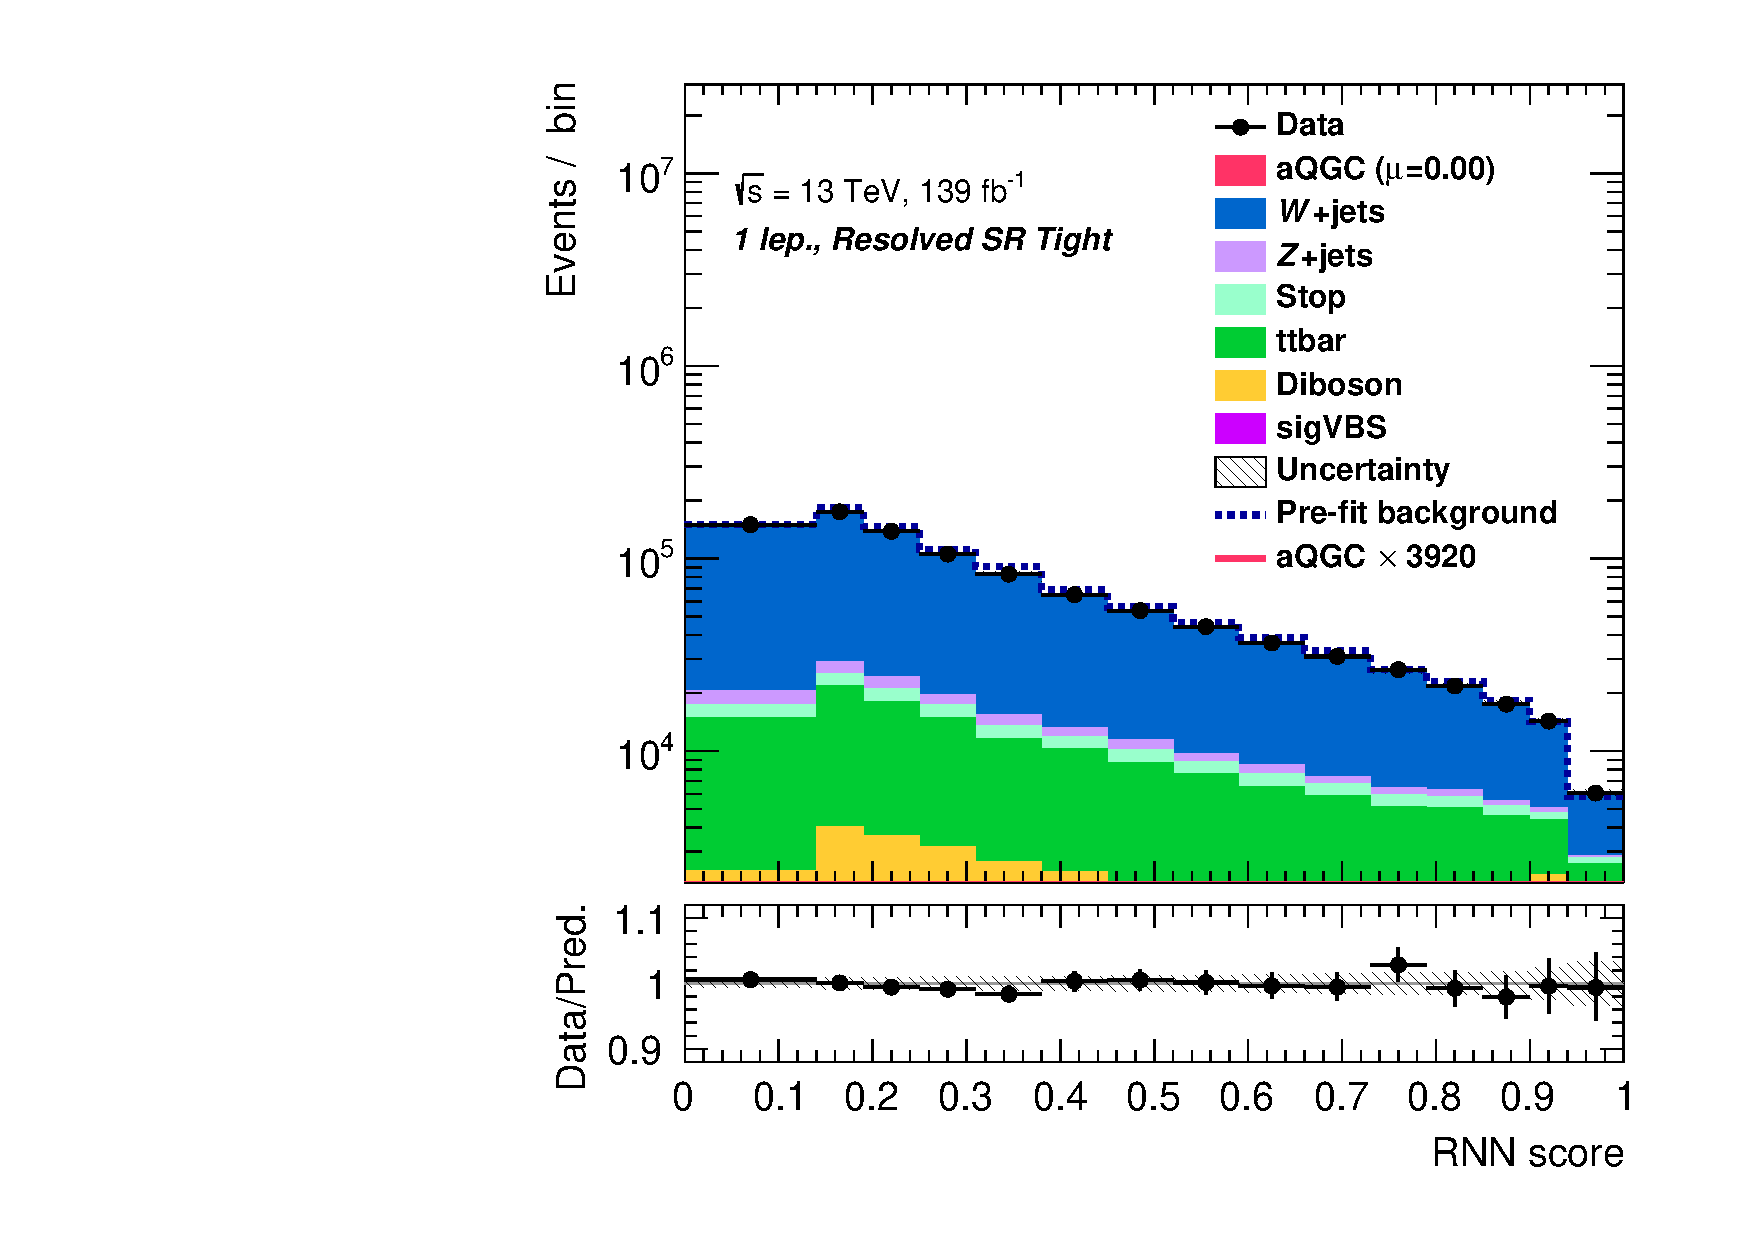
\includegraphics[width=0.45\textwidth]{figures/aQGC/PostFit/Region_distRNN_DSRVBSTightLMlvjj1500_BMin0_T0_Y6051_incTag1_J2_L1_incJet1_GlobalFit_unconditionnal_mu1log}
    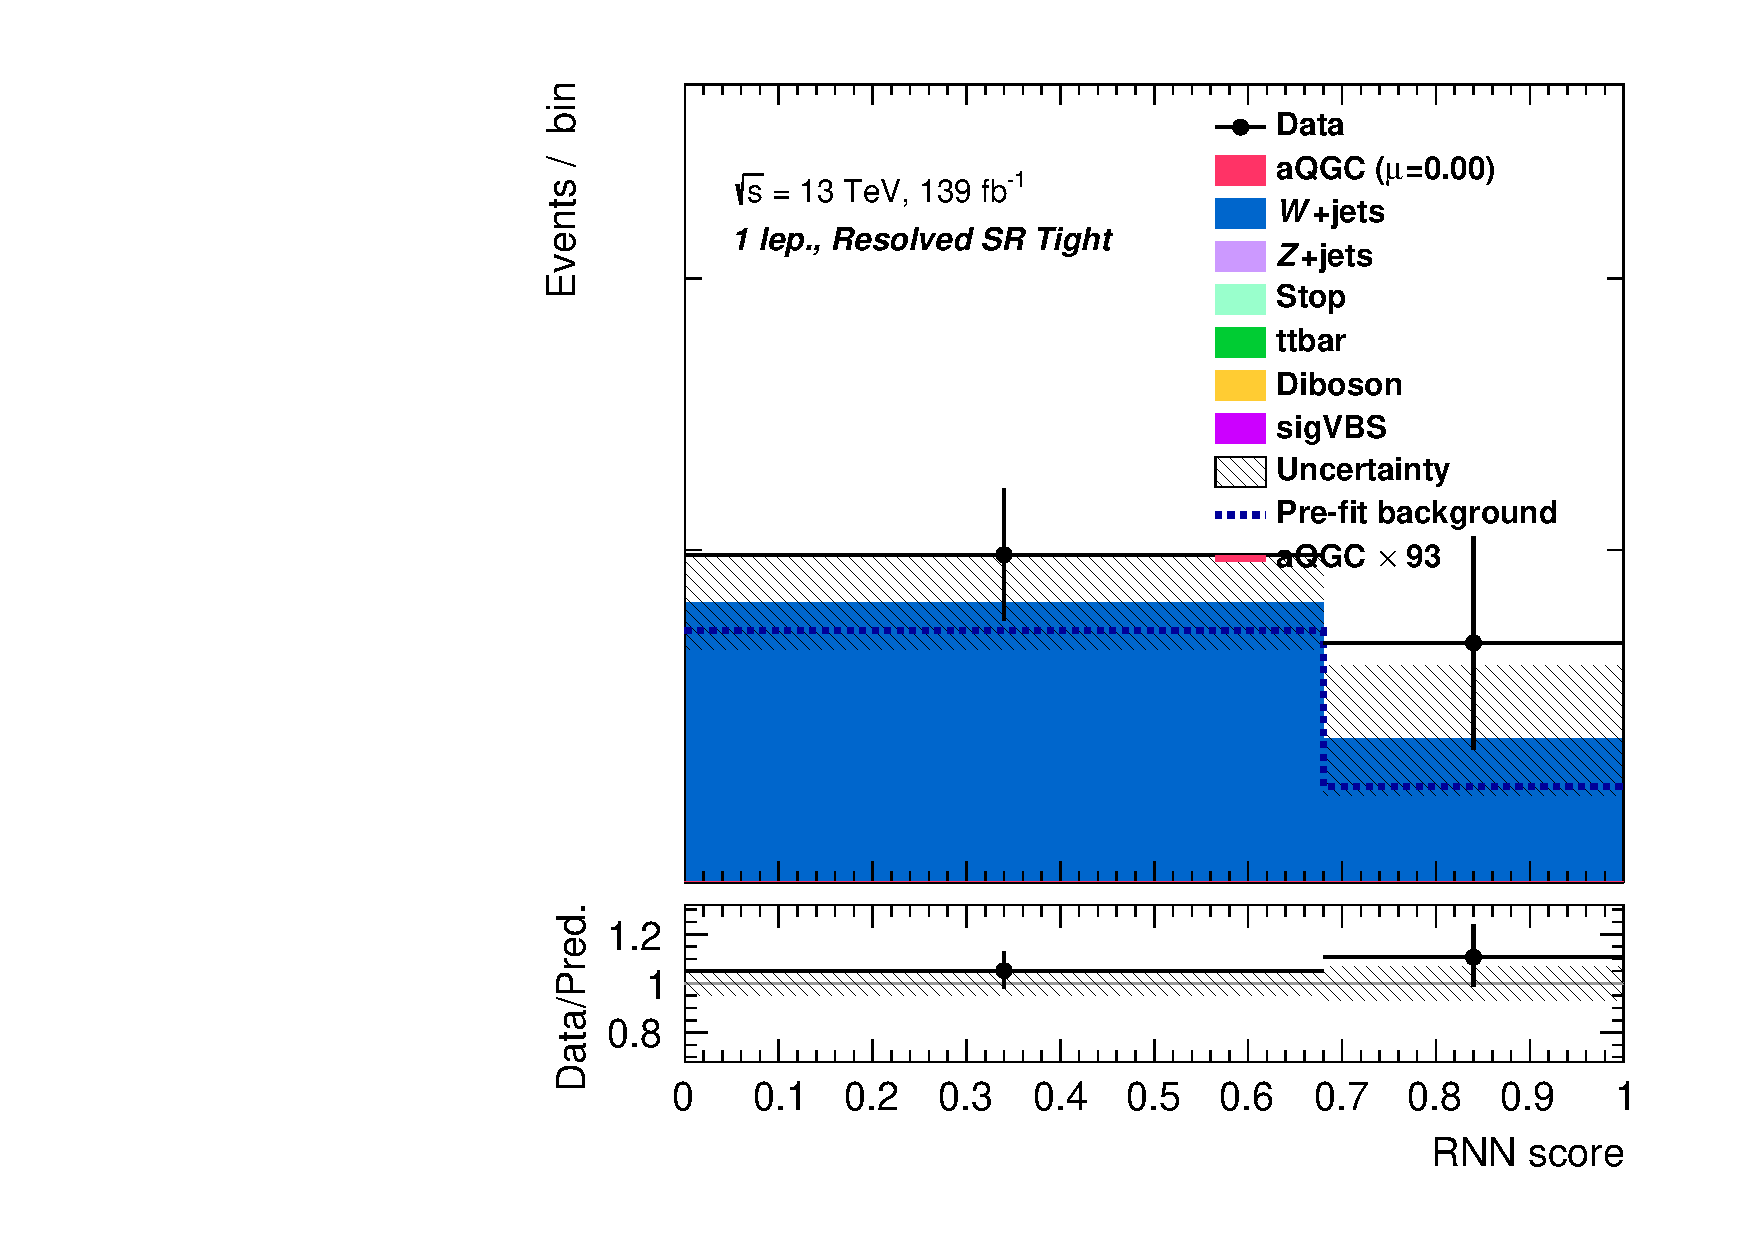
\includegraphics[width=0.45\textwidth]{figures/aQGC/PostFit/Region_distRNN_DSRVBSTightHMlvjj1500_BMin0_T0_Y6051_incTag1_J2_L1_incJet1_GlobalFit_unconditionnal_mu1log}
      \caption{Comparisons of the observed data and expected background distributions of RNN score in 1-lepton channel signal regions. Low-$m_{VV}$ region (left) and the high-$m_{VV}$ region (right) are shown.}
      \label{fig:postSR1lepaQGC}
\end{figure}
\begin{figure}[]
    \centering
    %2lep
    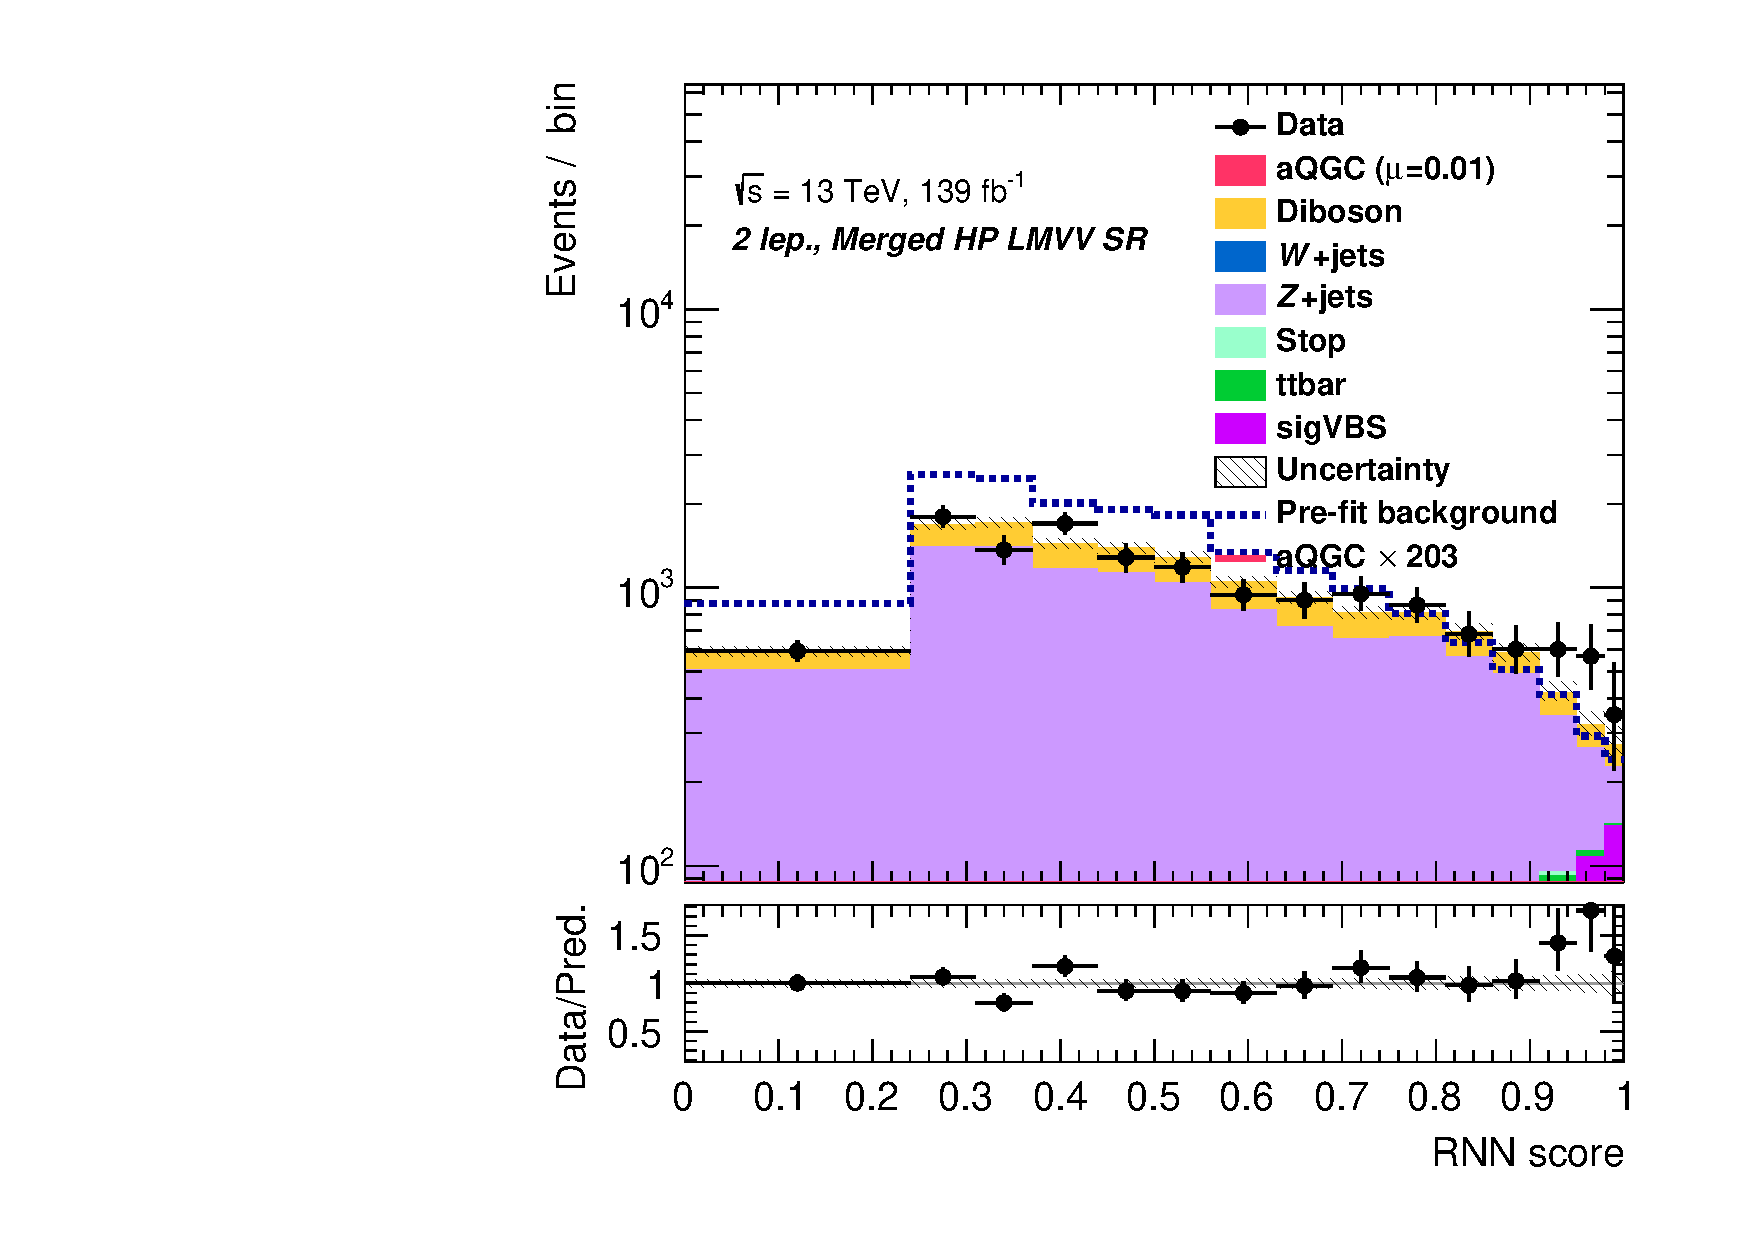
\includegraphics[width=0.45\textwidth]{figures/aQGC/PostFit/Region_distRNNScoreMerged_DSRVBSHPLMllJ1500_BMin0_J0_incJet1_L2_T0_incFat1_Y6051_incTag1_Fat1_GlobalFit_unconditionnal_mu1log}
    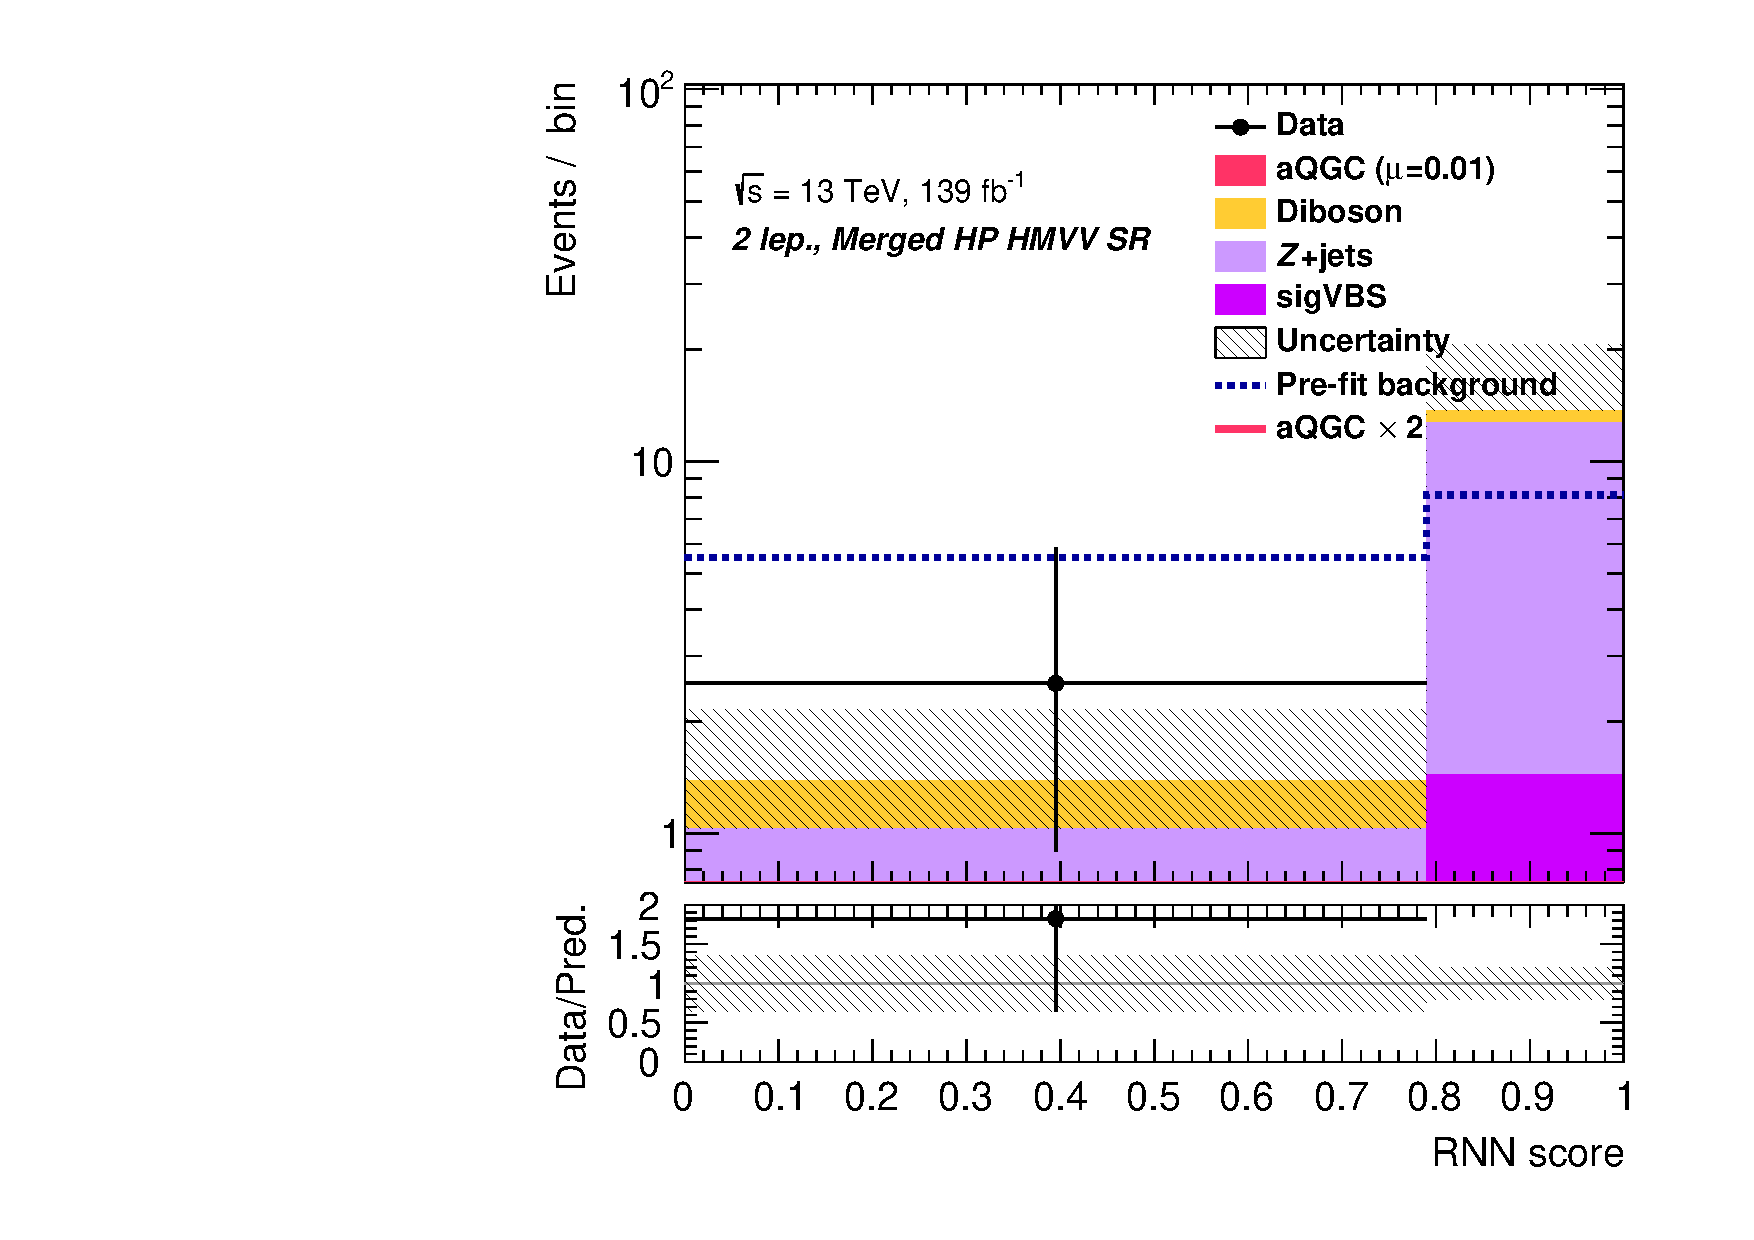
\includegraphics[width=0.45\textwidth]{figures/aQGC/PostFit/Region_distRNNScoreMerged_DSRVBSHPHMllJ1500_BMin0_J0_incJet1_L2_T0_incFat1_Y6051_incTag1_Fat1_GlobalFit_unconditionnal_mu1log}
    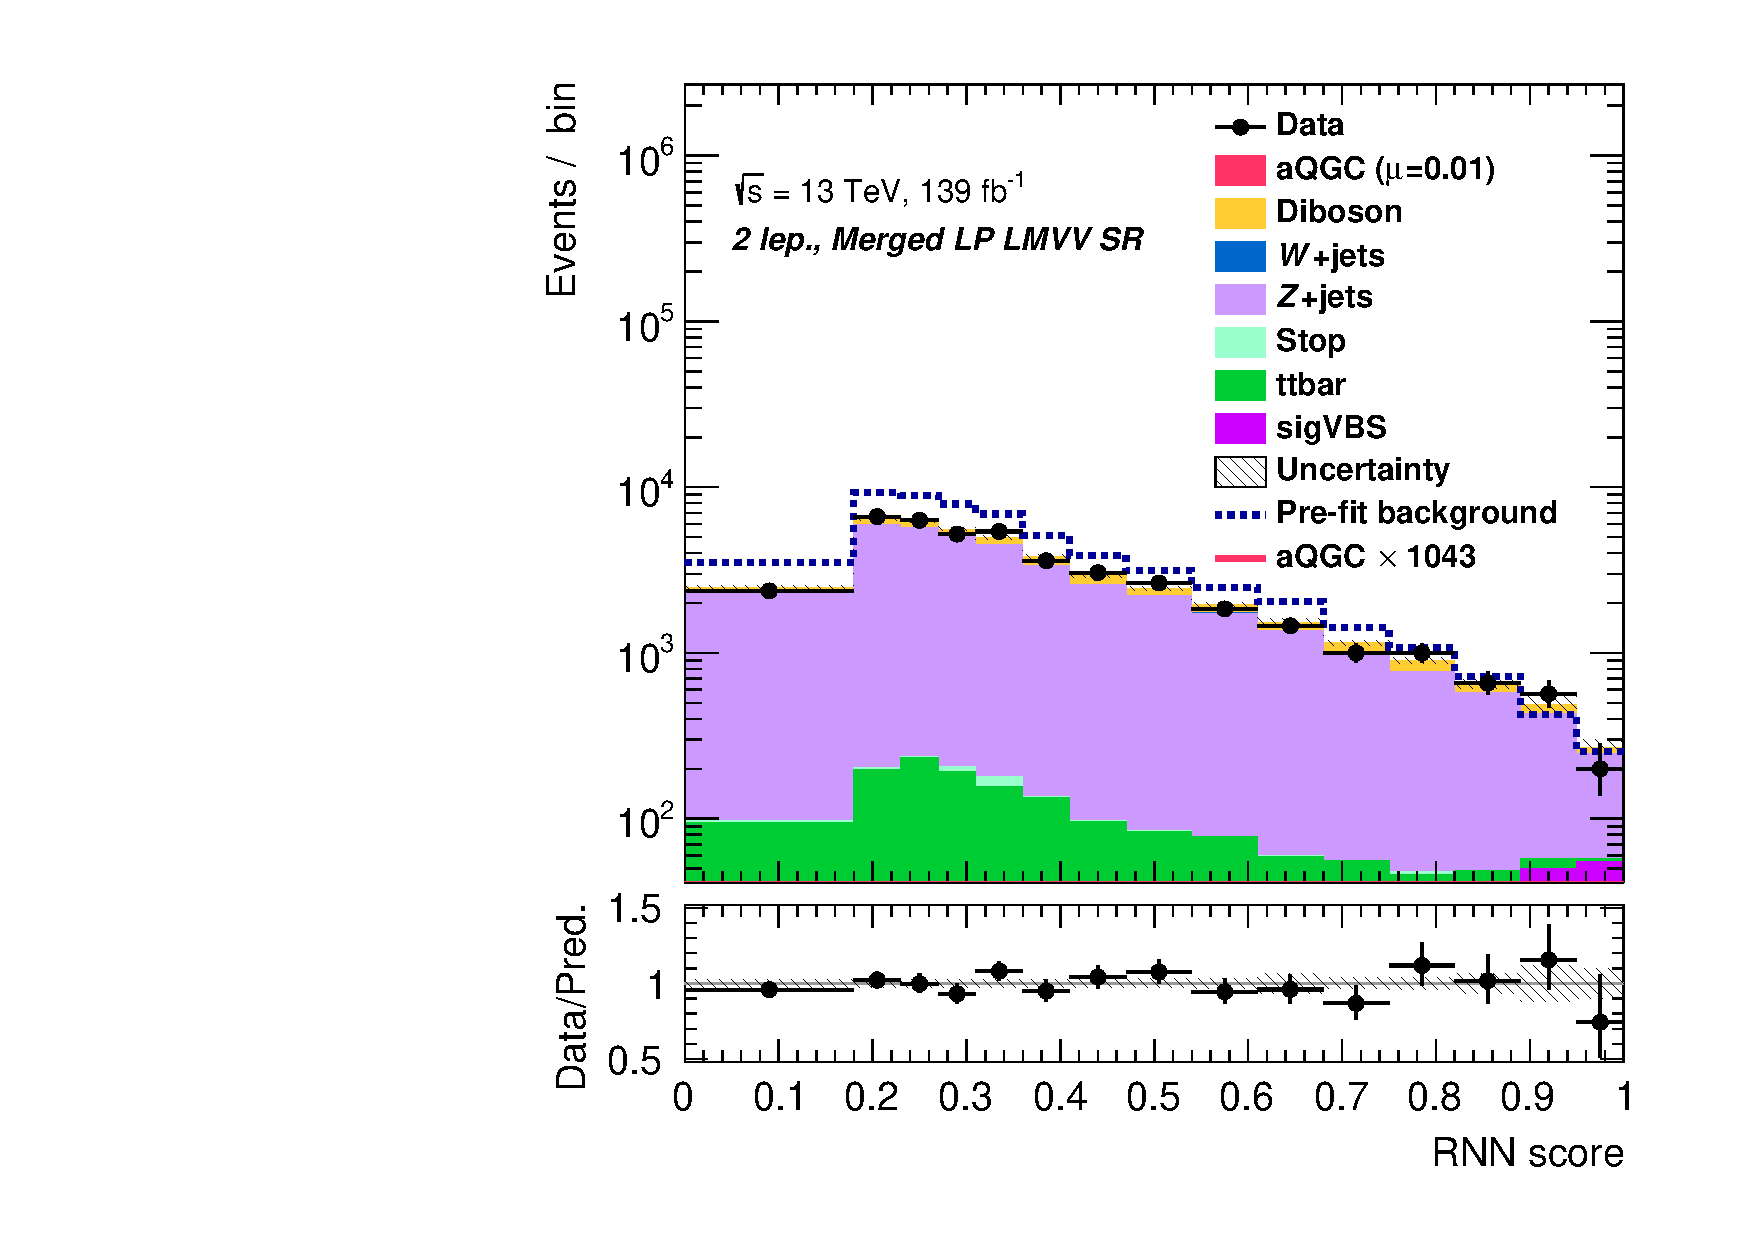
\includegraphics[width=0.45\textwidth]{figures/aQGC/PostFit/Region_distRNNScoreMerged_DSRVBSLPLMllJ1500_BMin0_J0_incJet1_L2_T0_incFat1_Y6051_incTag1_Fat1_GlobalFit_unconditionnal_mu1log}
    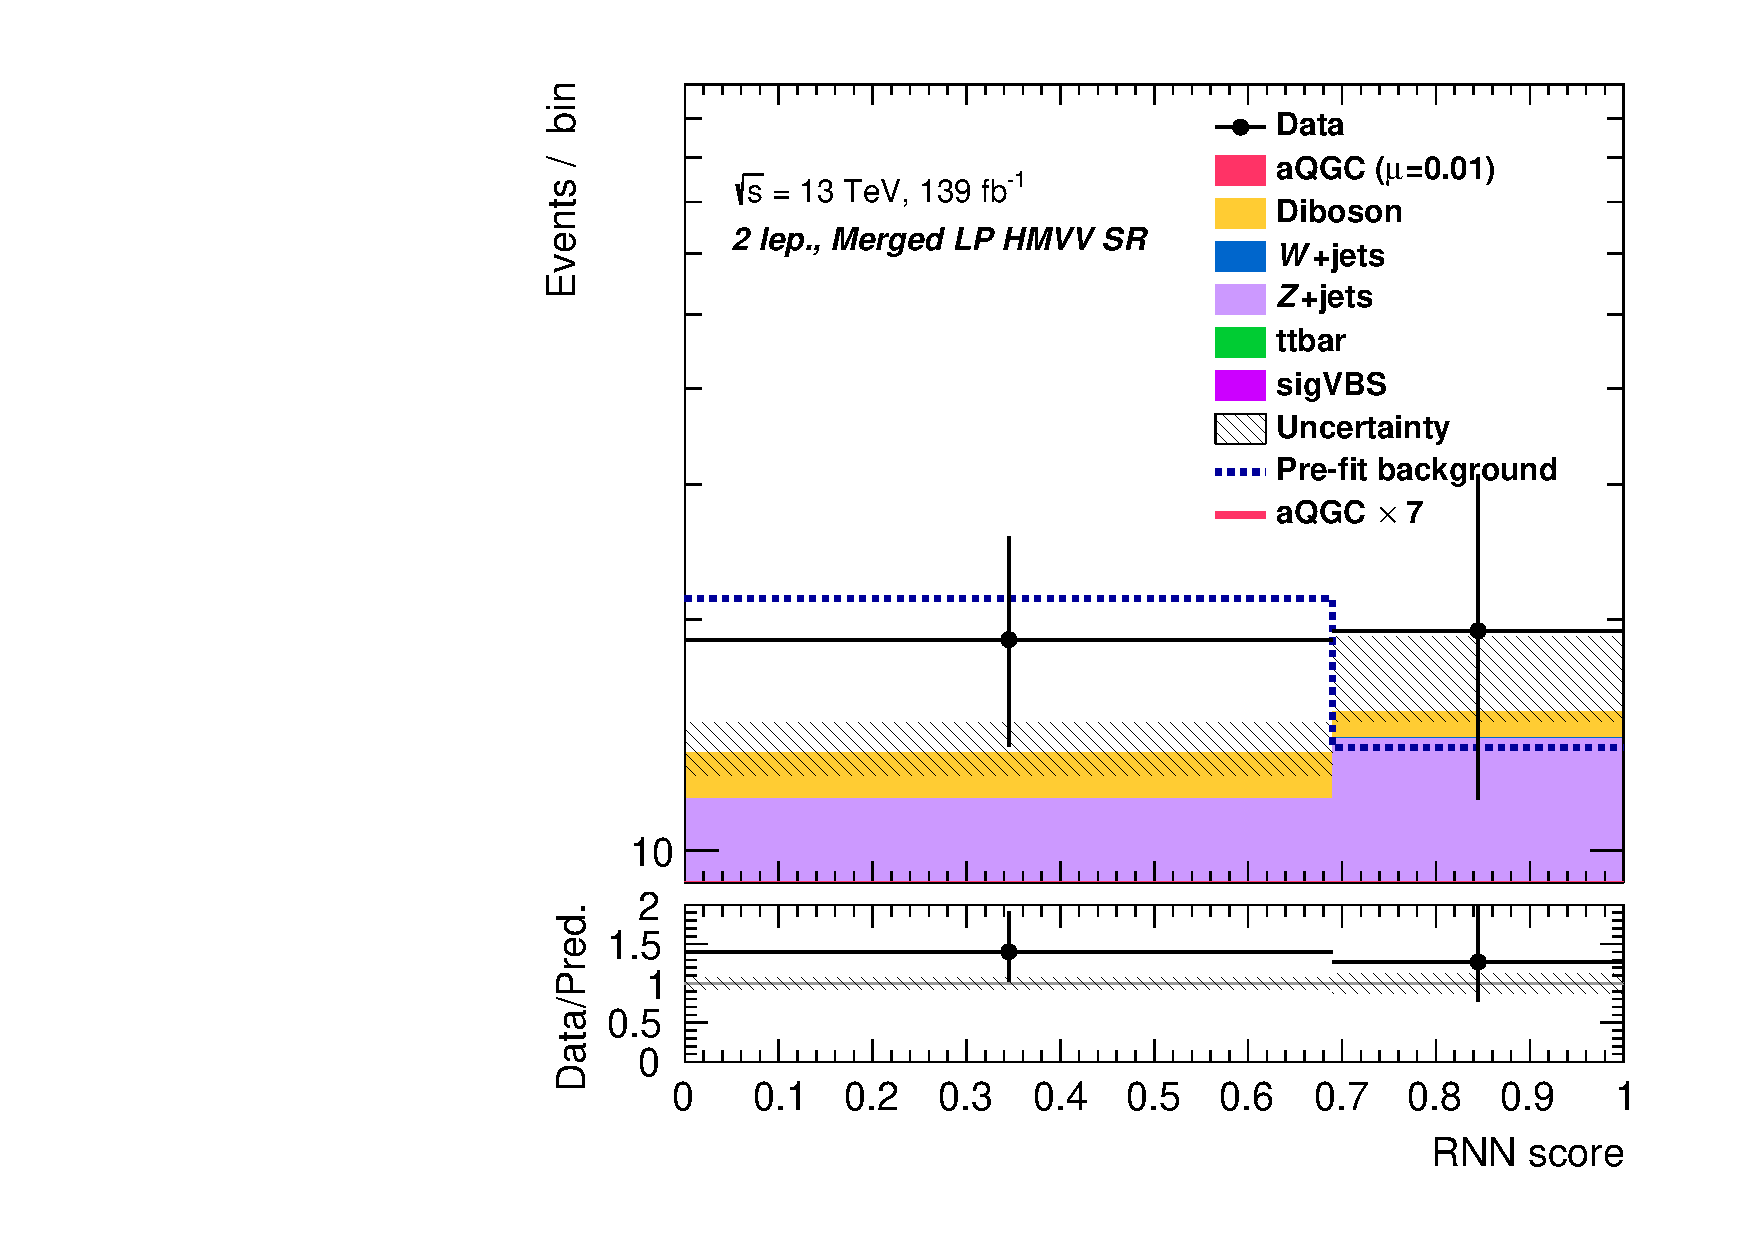
\includegraphics[width=0.45\textwidth]{figures/aQGC/PostFit/Region_distRNNScoreMerged_DSRVBSLPHMllJ1500_BMin0_J0_incJet1_L2_T0_incFat1_Y6051_incTag1_Fat1_GlobalFit_unconditionnal_mu1log}
    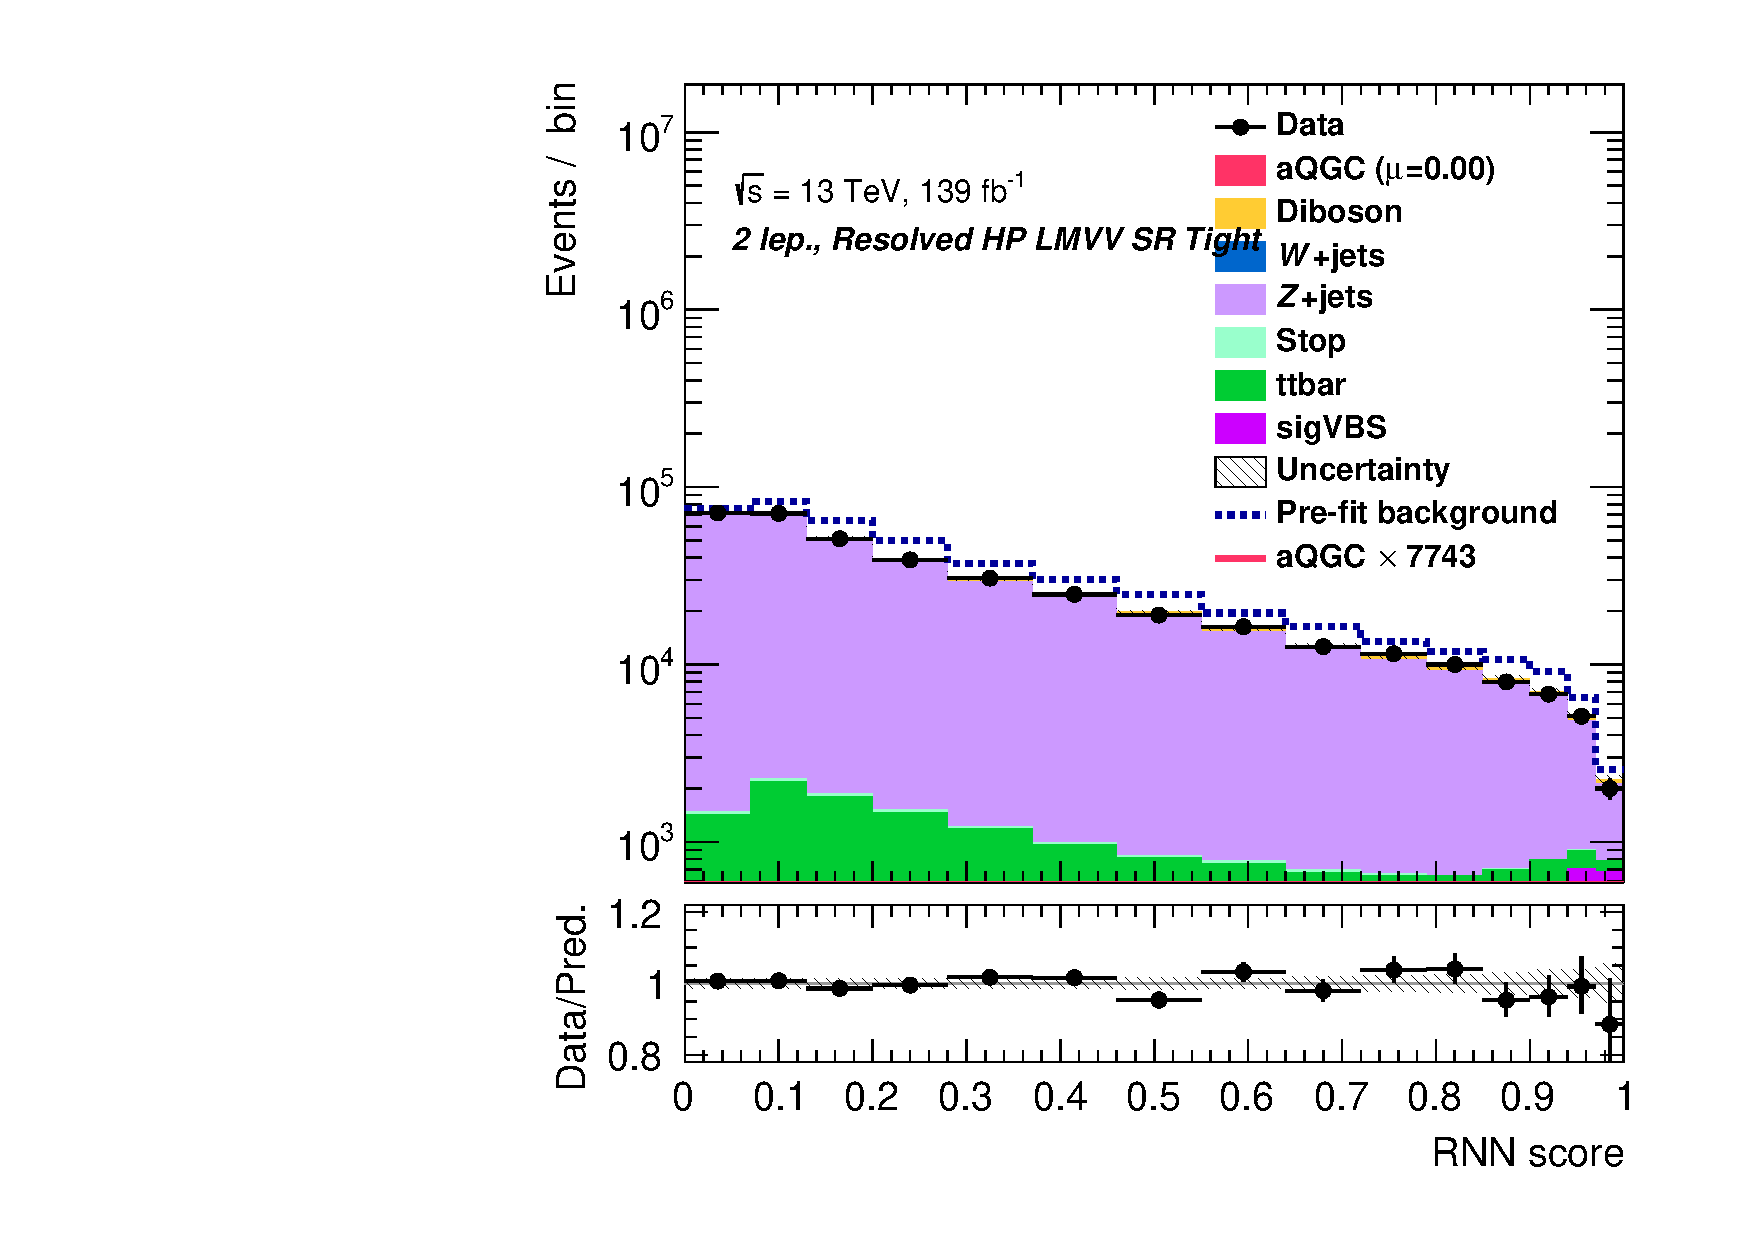
\includegraphics[width=0.45\textwidth]{figures/aQGC/PostFit/Region_distRNNScoreResolved_DSRVBSFidLMlljj1500_BMin0_T0_Y6051_incTag1_J2_L2_incJet1_GlobalFit_unconditionnal_mu1log}
    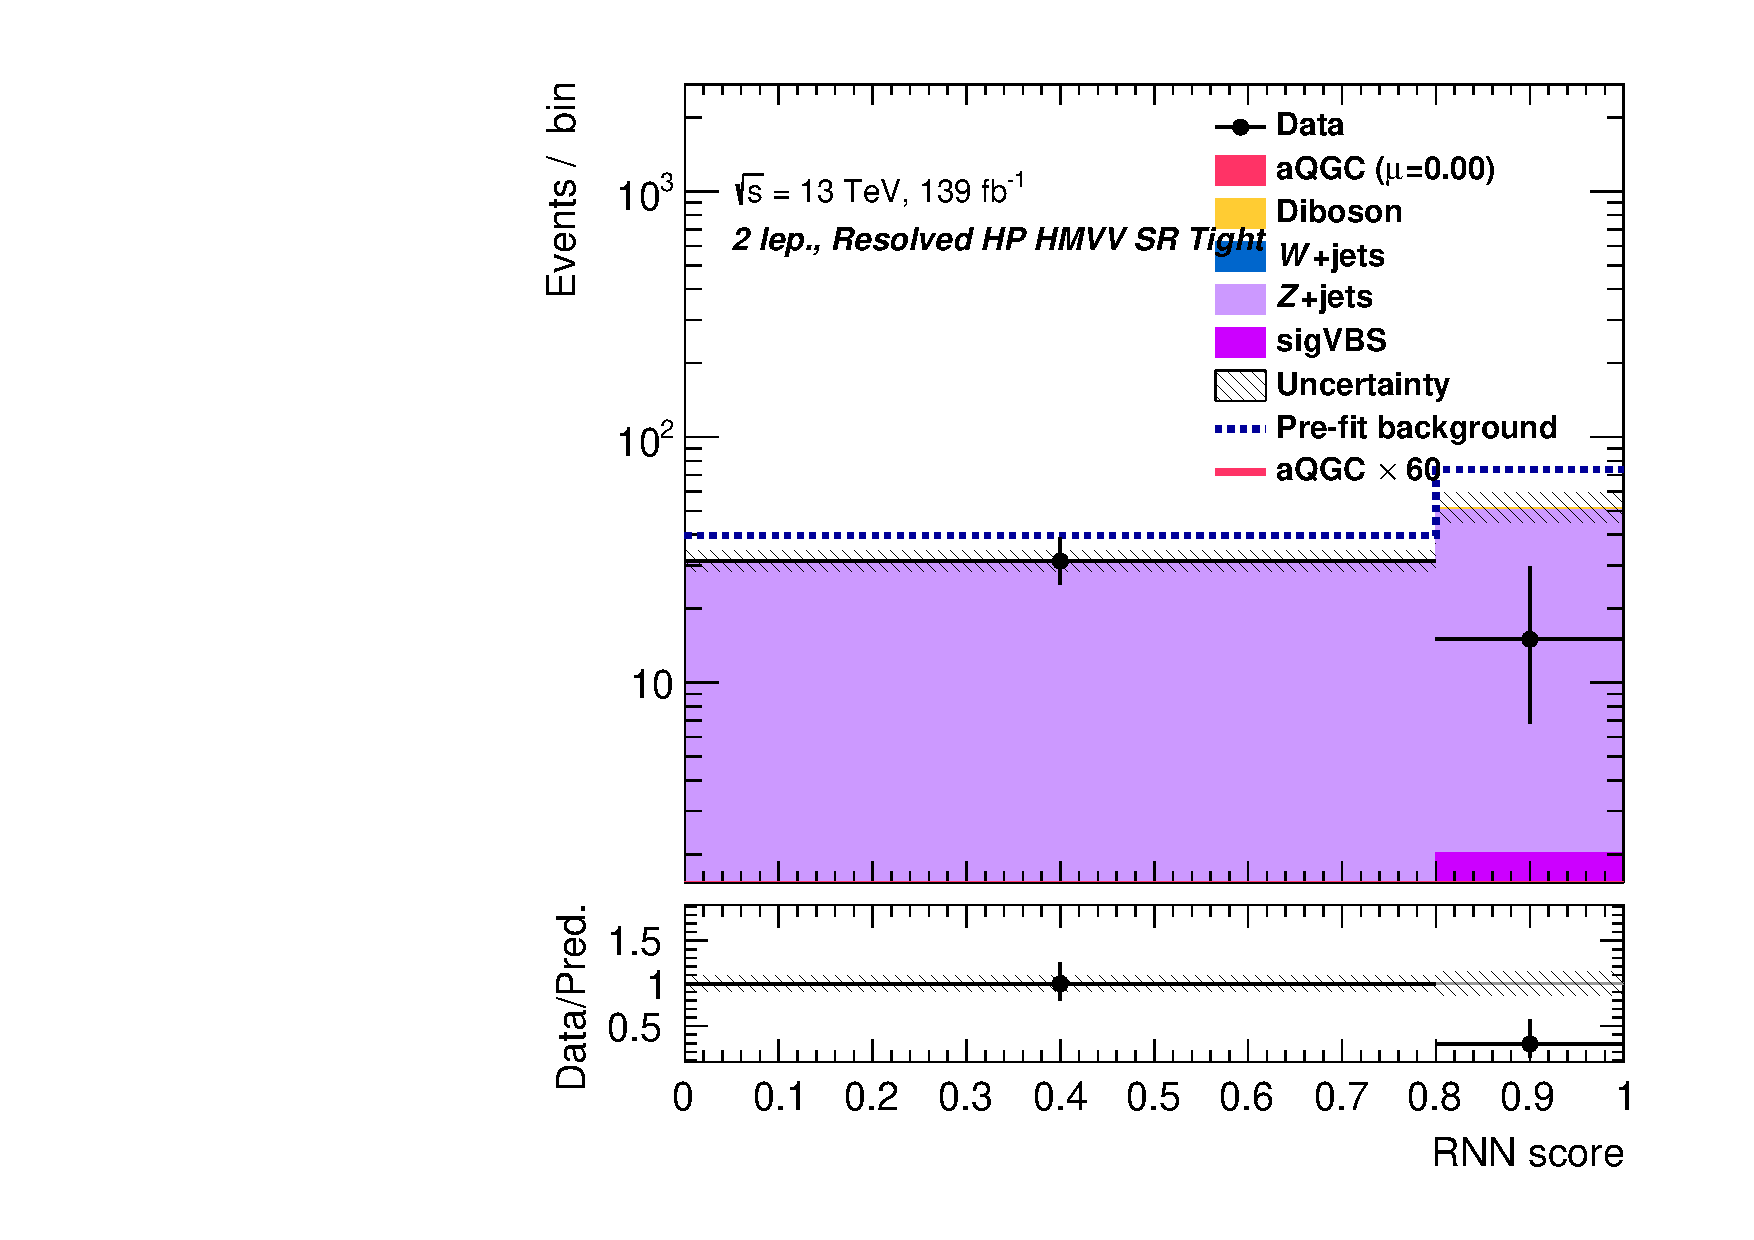
\includegraphics[width=0.45\textwidth]{figures/aQGC/PostFit/Region_distRNNScoreResolved_DSRVBSFidHMlljj1500_BMin0_T0_Y6051_incTag1_J2_L2_incJet1_GlobalFit_unconditionnal_mu1log}
    \caption{Comparisons of the observed data and expected background distributions of RNN score in 2-lepton channel signal regions. Low-$m_{VV}$ region (left) and the high-$m_{VV}$ region (right) are shown. }
    \label{fig:postSR2lepaQGC}
\end{figure}

The expected and observed limits are shown at 5 clipping energy points of [1.5, 2.0, 3.0, 5.0, $\infty$]~TeV in Figure~\ref{fig:aQGClimits}.
The unitarity bound from the theoretical calculation \cite{PhysRevD.101.113003} is overlaid.
%The upper and lower limits correspond to the signal hypotheses showing $\Delta NLL \sim \frac{1}{2}\chi^2 = 1.0$.
The log-likelihood (-2 ln $\lambda$; $\lambda$ is a likelihood ratio) distributions with respect to the $\mu_\mathrm{aQGC}$, is shown in figure~\ref{fig:ProfileLL},\ref{fig:ProfileLLFS}, \ref{fig:ProfileLLFM} for FT0, FS02, FM0 operator, for each clipping energy of 1500~GeV, 2000~GeV, $\infty$.
%Figure~\ref{}, \ref{}, \ref{} show the log-likelihood curve obtained by the fitting with observed data for each clipping energy, for FT0, FS02, FM0 operators, respectively.
\begin{figure}[ht]
    \centering
    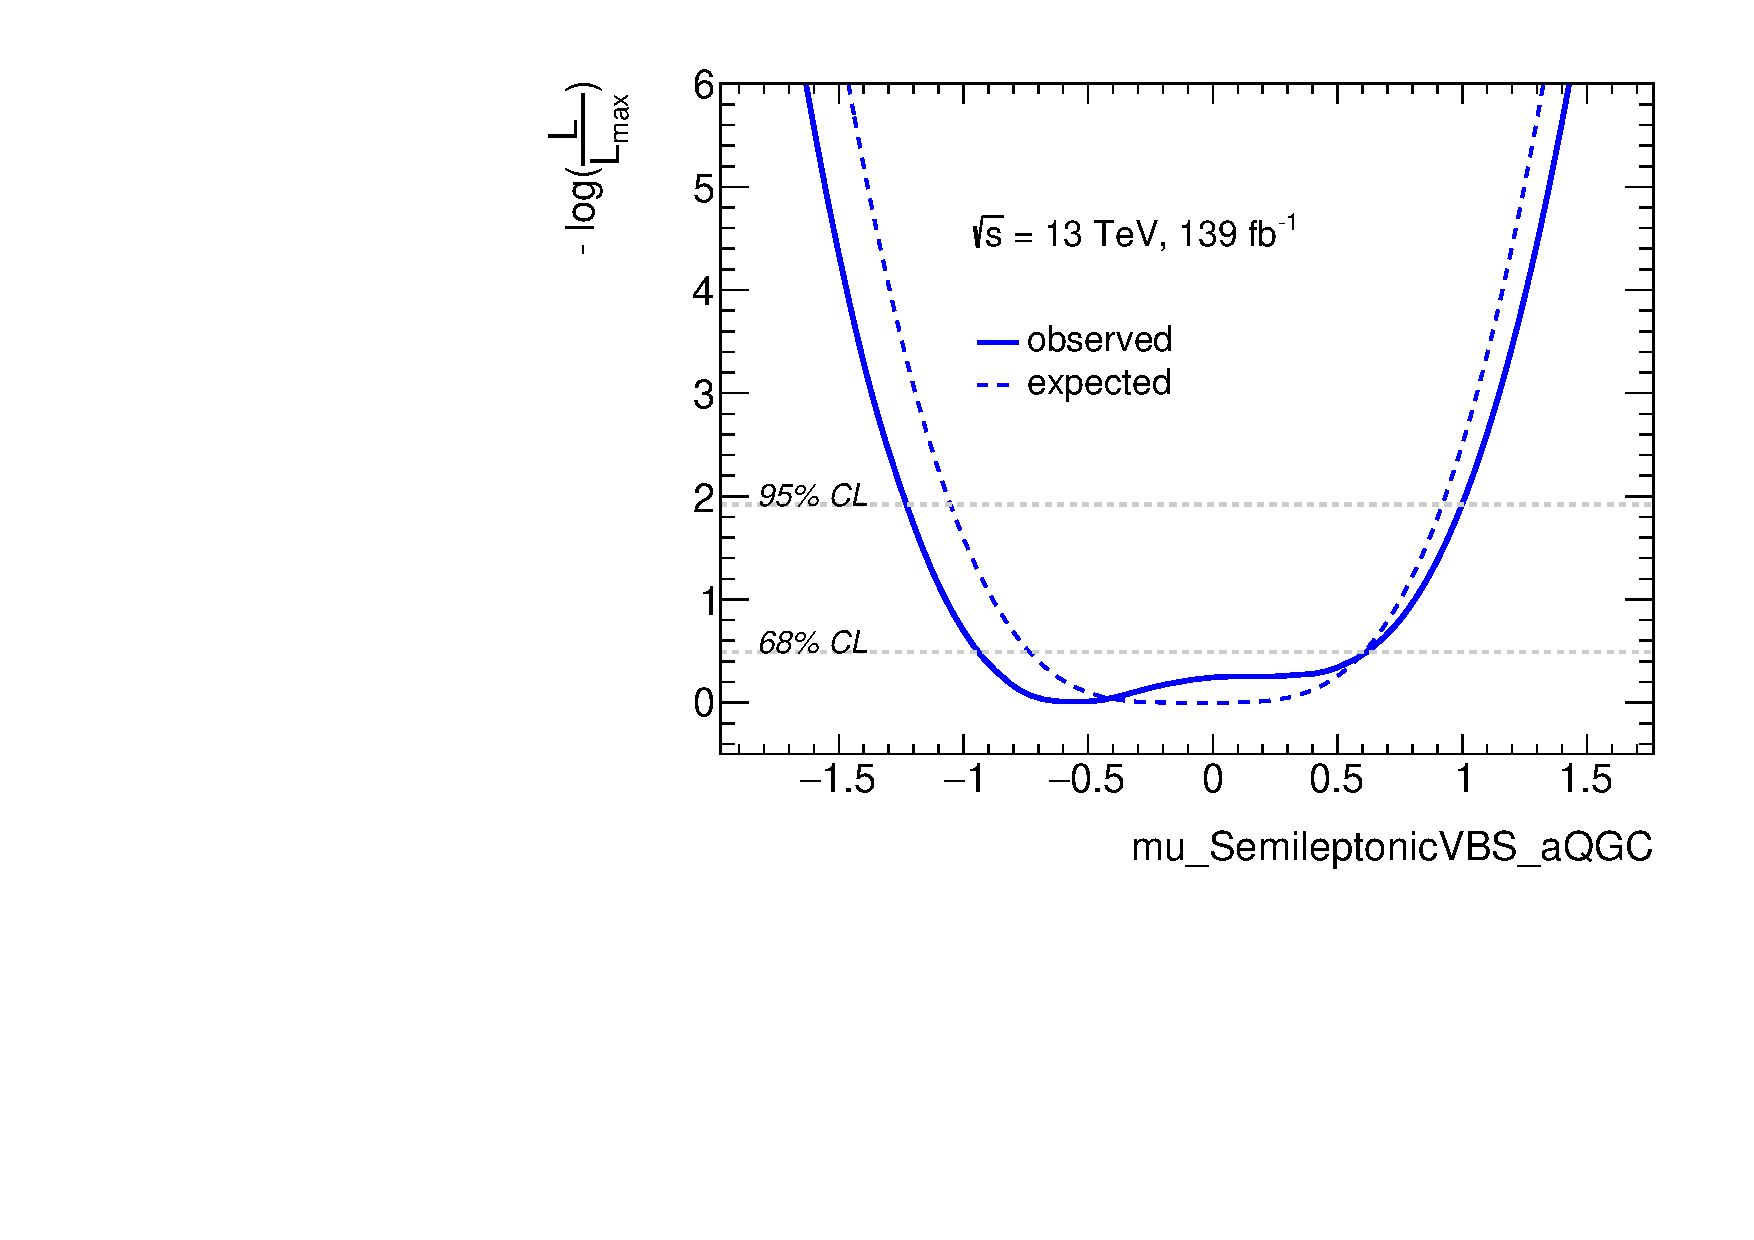
\includegraphics[width=0.32\textwidth]{figures/aQGC/profileFT01500}
    	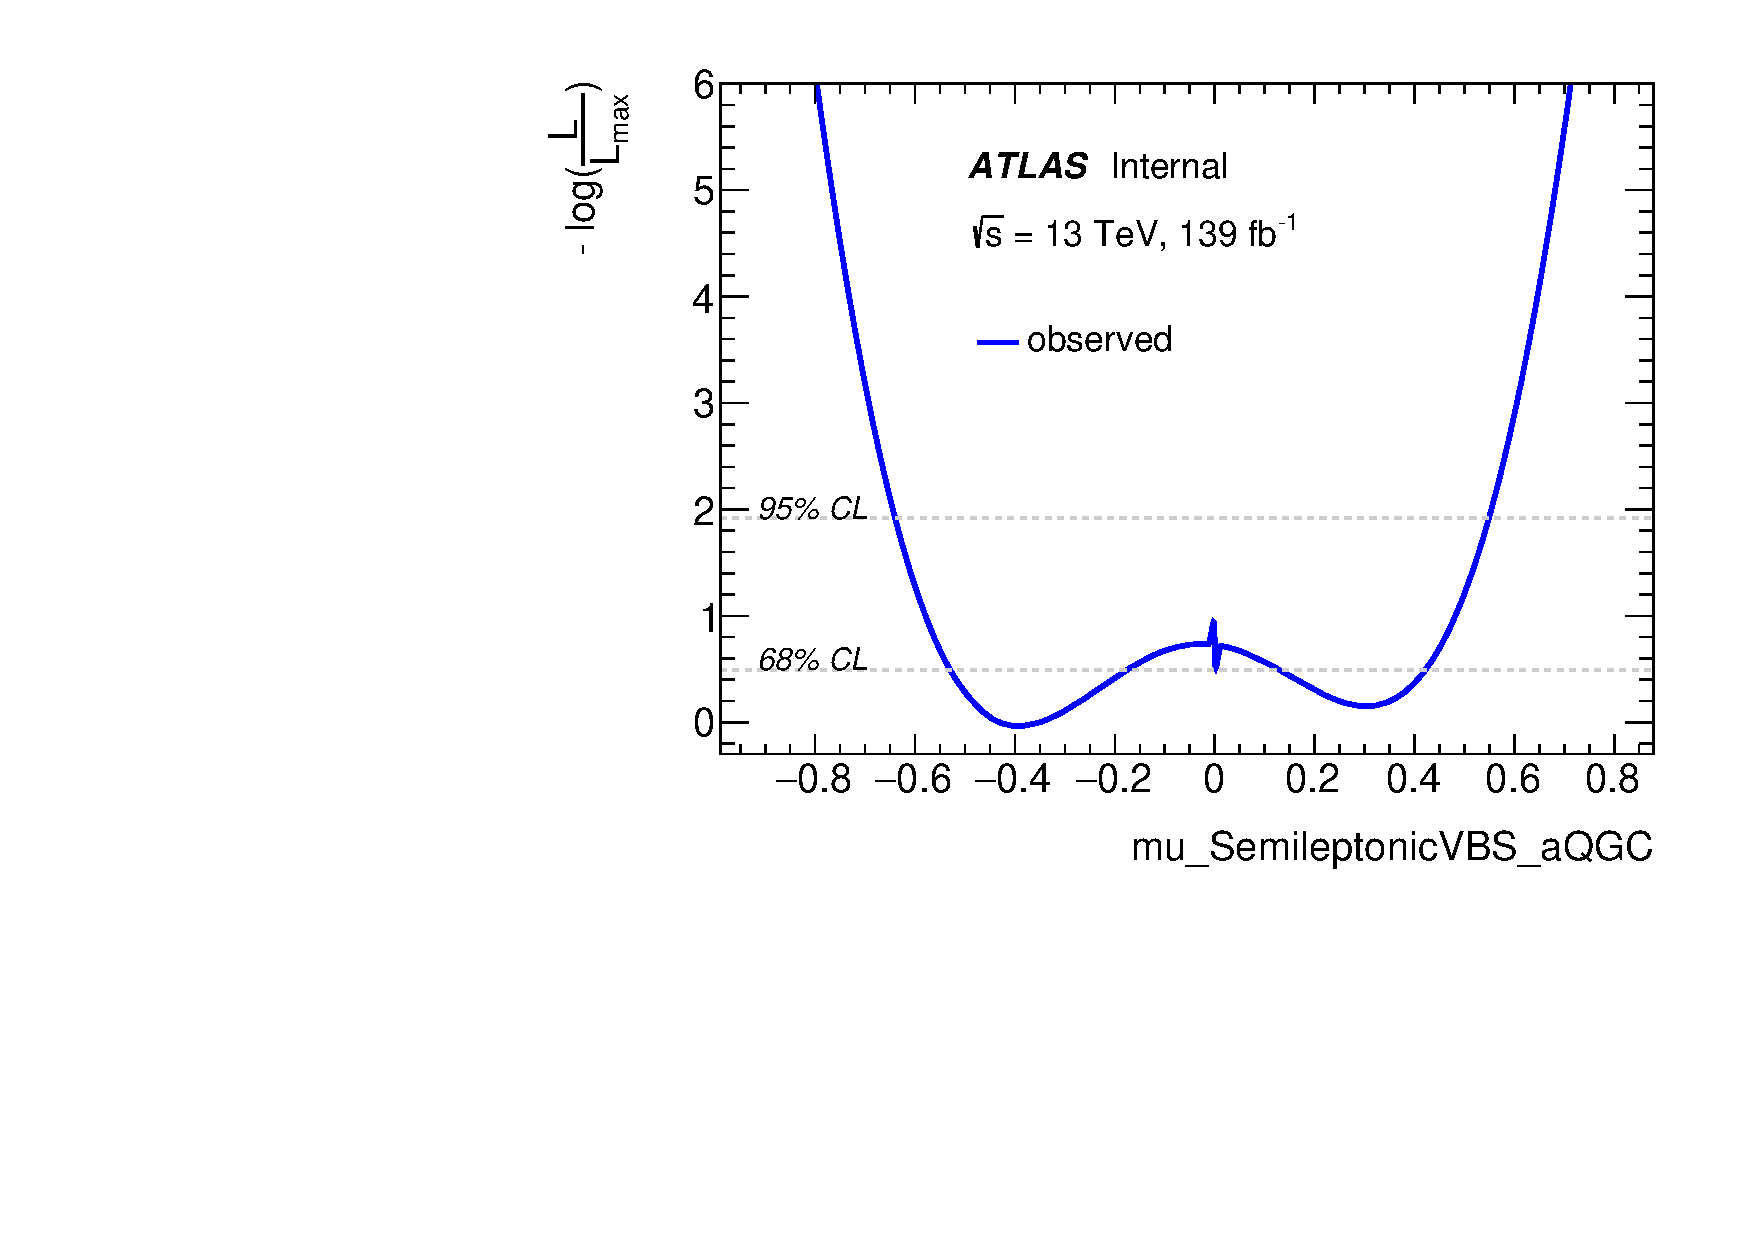
\includegraphics[width=0.32\textwidth]{figures/aQGC/profileFT02000}
    	%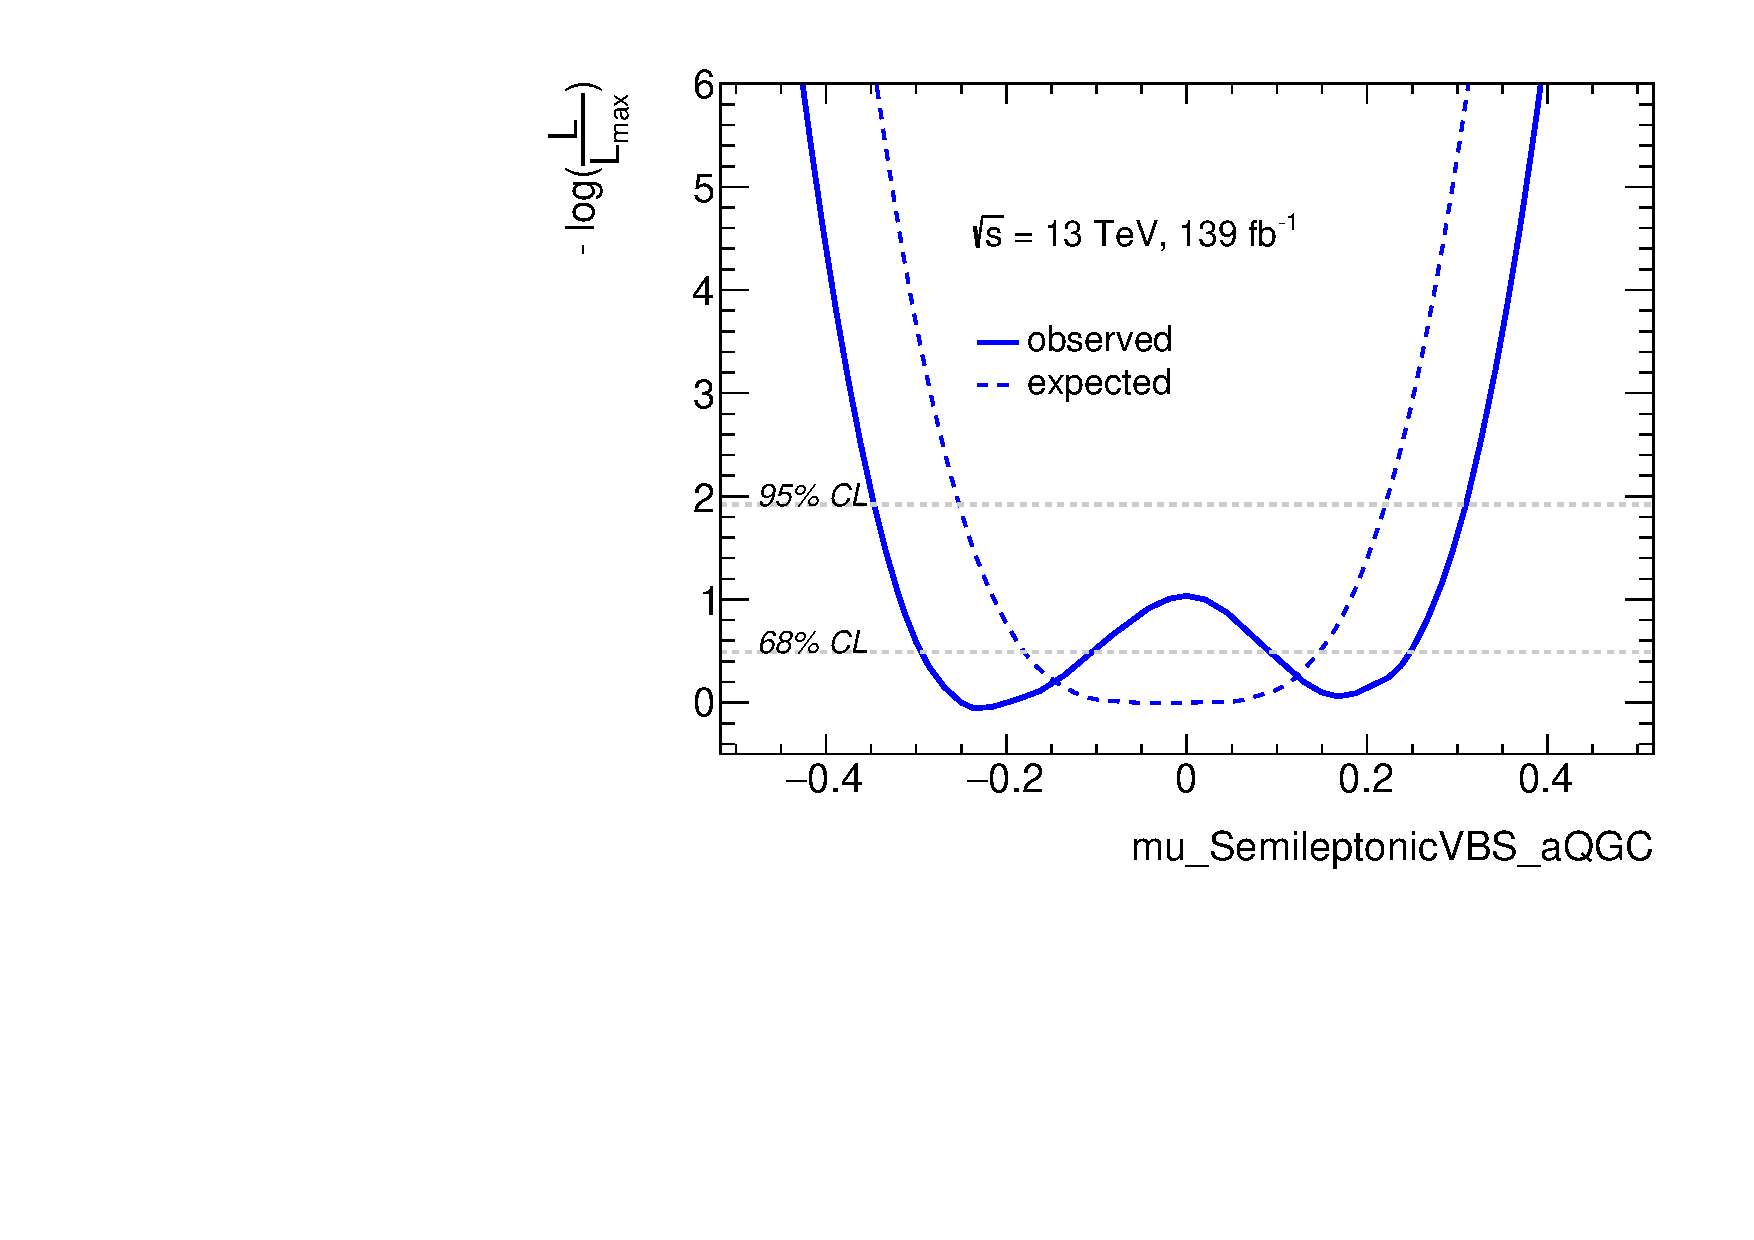
\includegraphics[width=0.38\textwidth]{figures/aQGC/profileFT03000}
        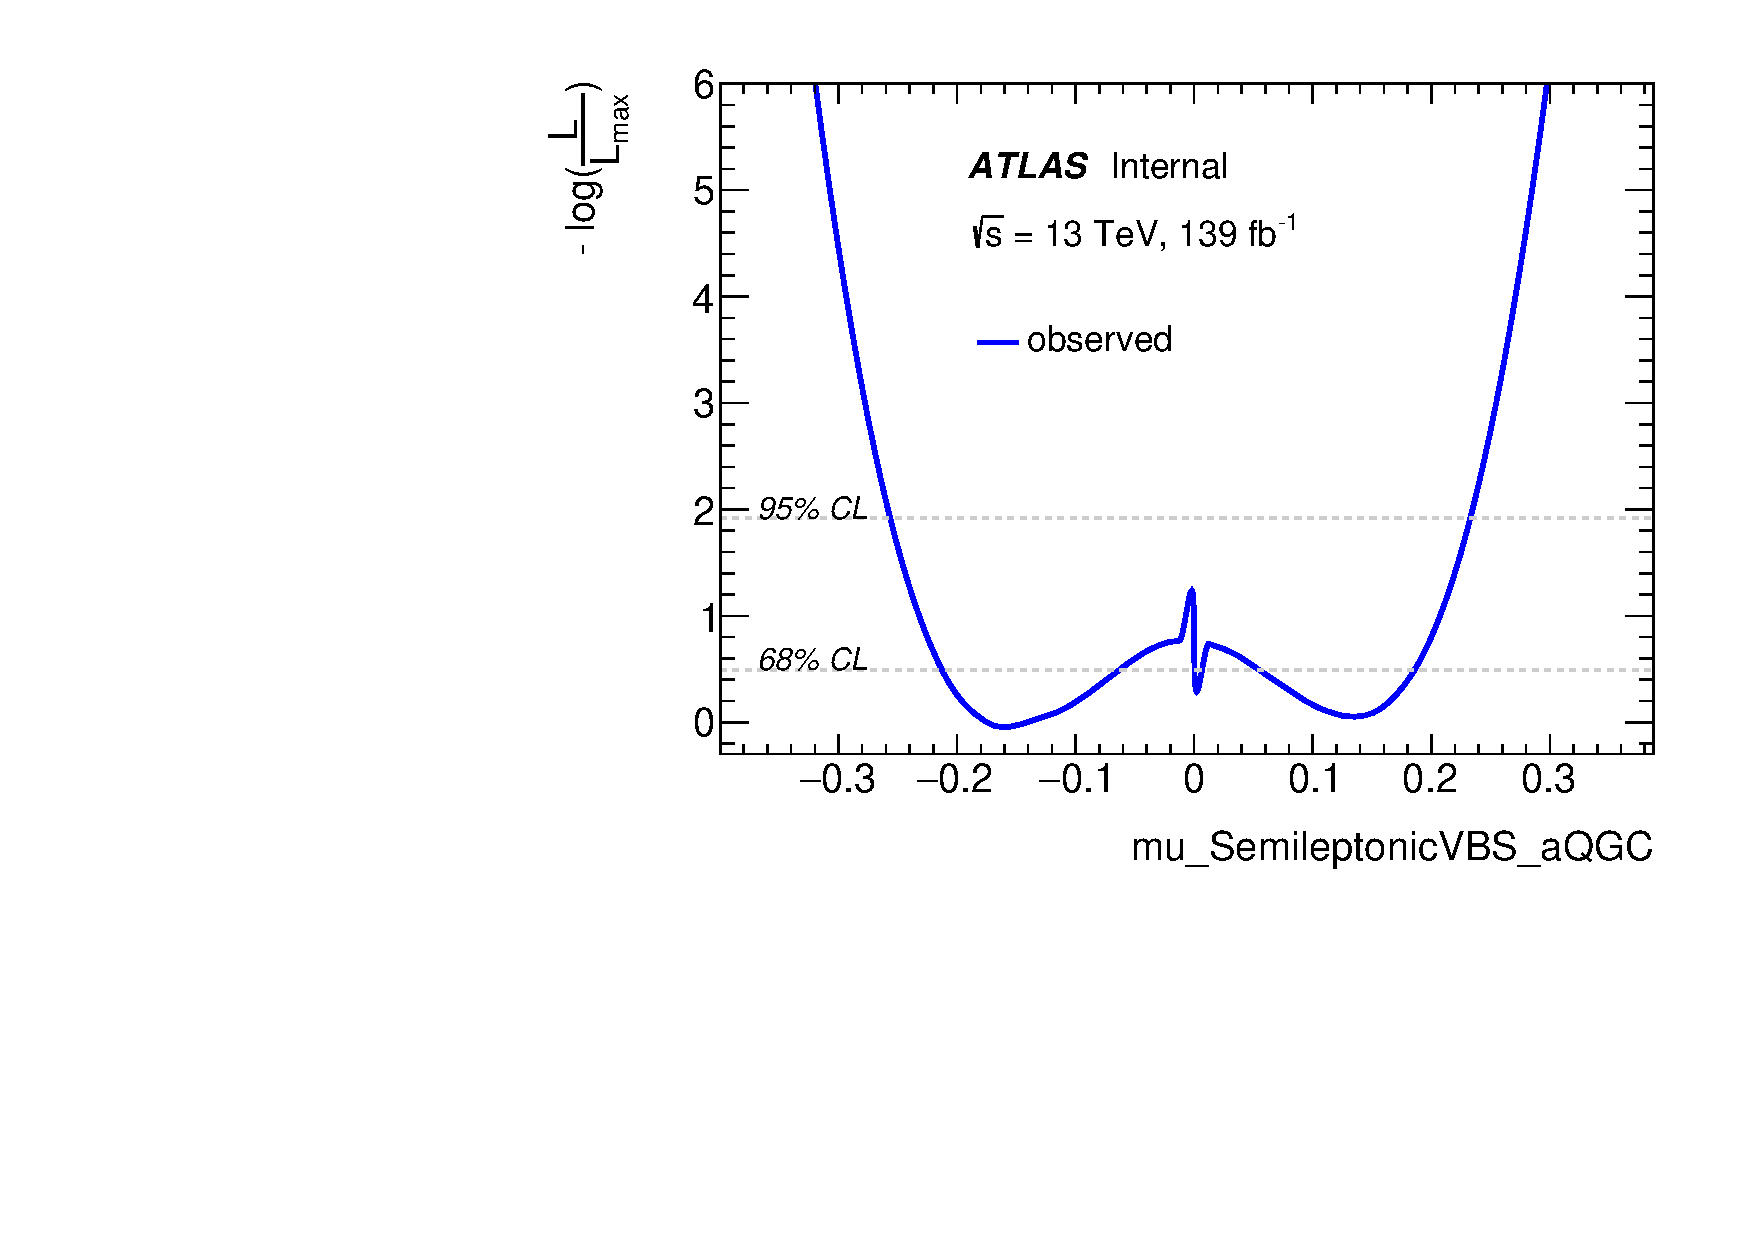
\includegraphics[width=0.32\textwidth]{figures/aQGC/profileFT0inf}
        \caption{The observed log-likelihood curves of FT0 Wilson coefficient where the clipping energy is 1.5~TeV (left), 2.0~TeV (middle), $\infty$ (right).}
        \label{fig:ProfileLL}
\end{figure}
\begin{figure}[ht]
    \centering
    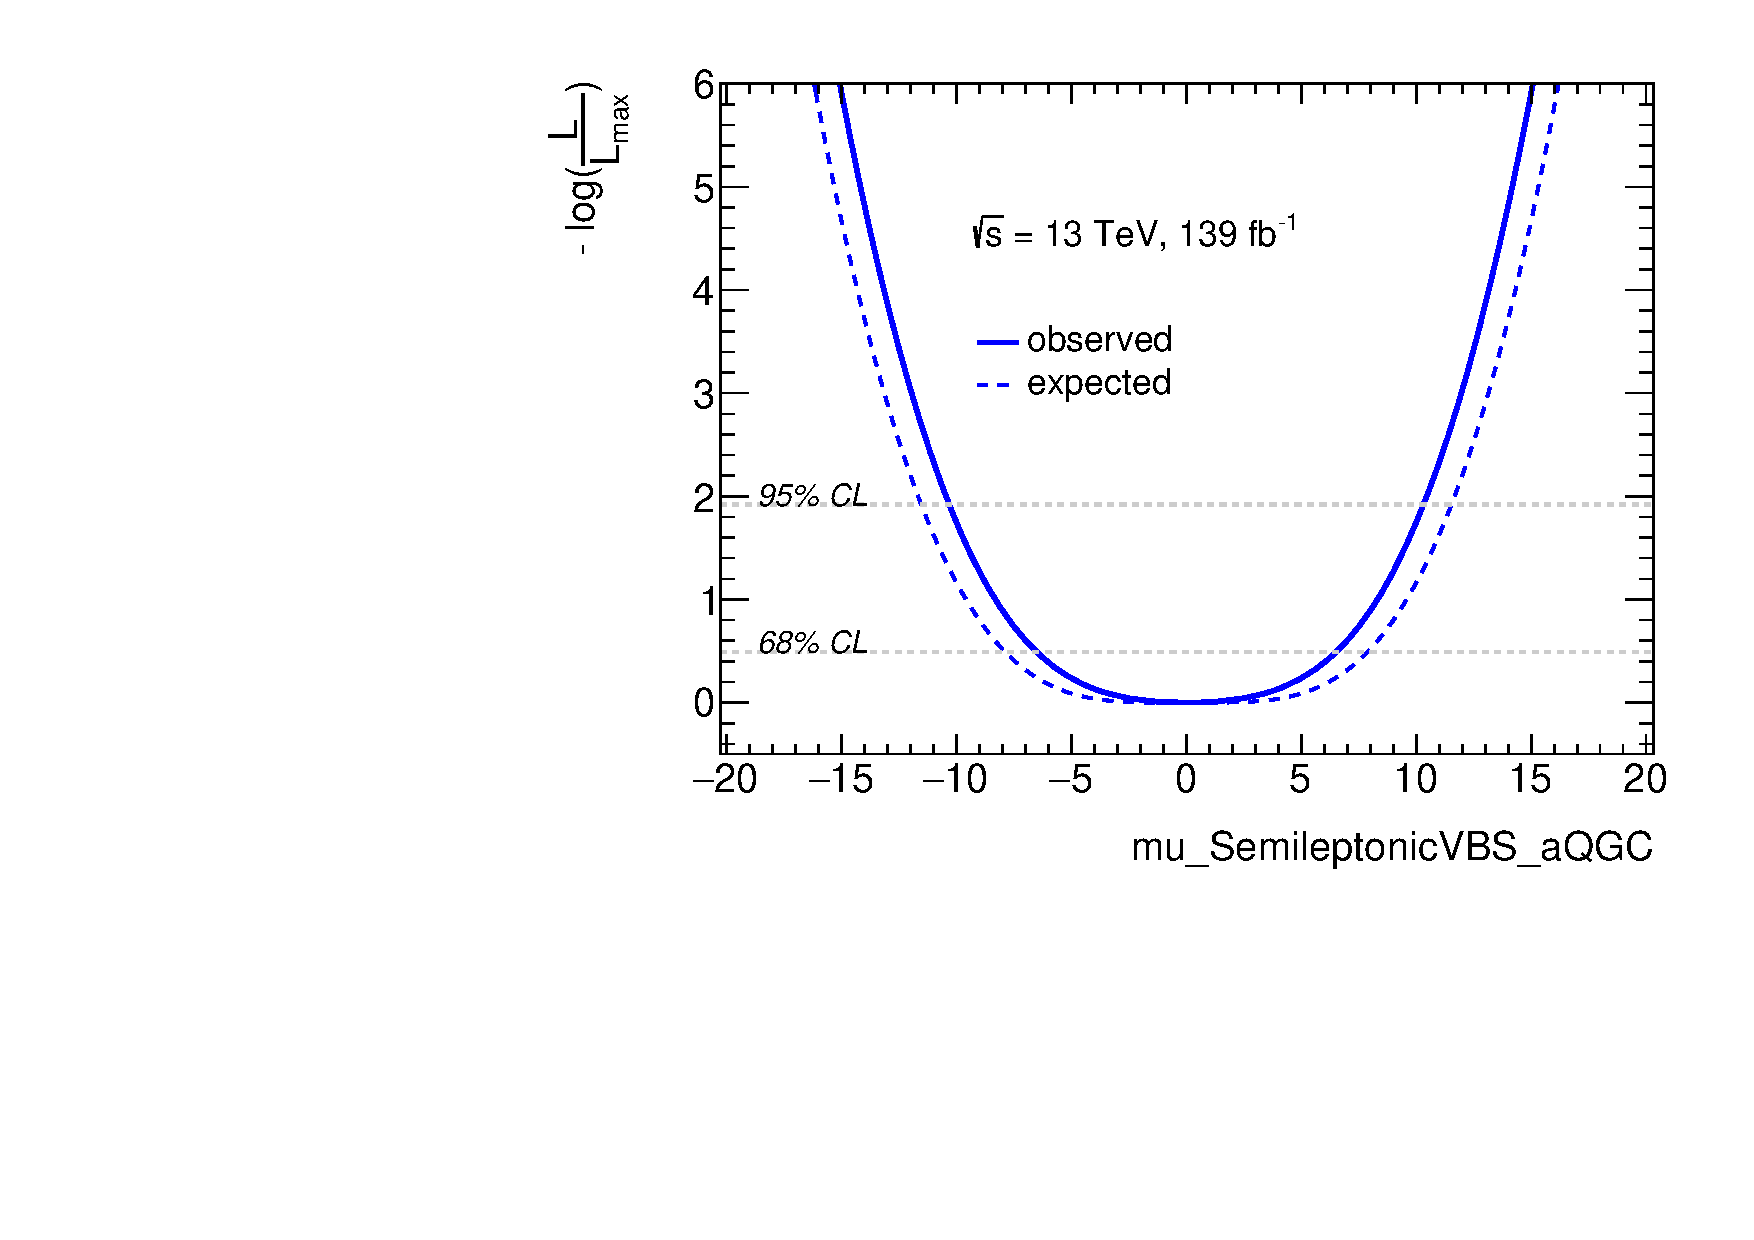
\includegraphics[width=0.32\textwidth]{figures/aQGC/profileFS021500}
    	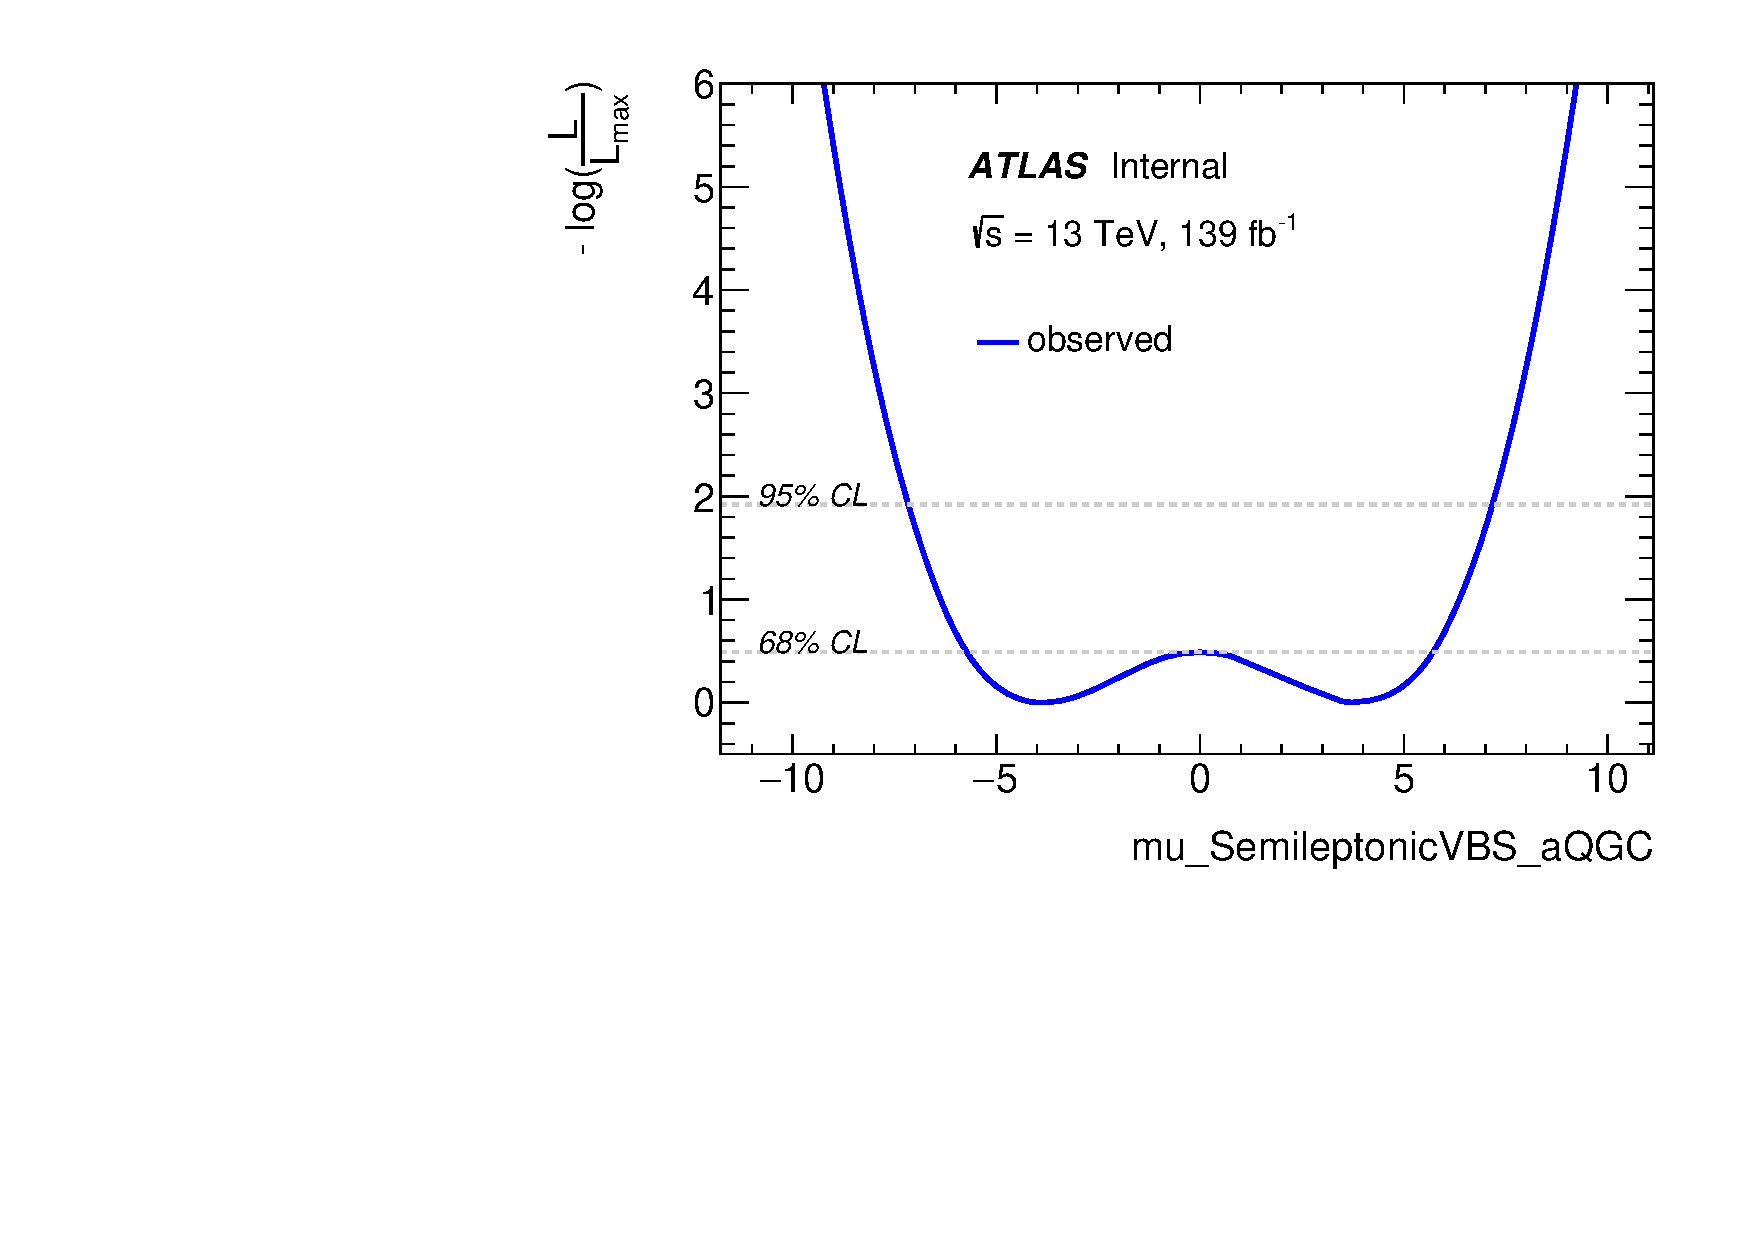
\includegraphics[width=0.32\textwidth]{figures/aQGC/profileFS022000}
    	%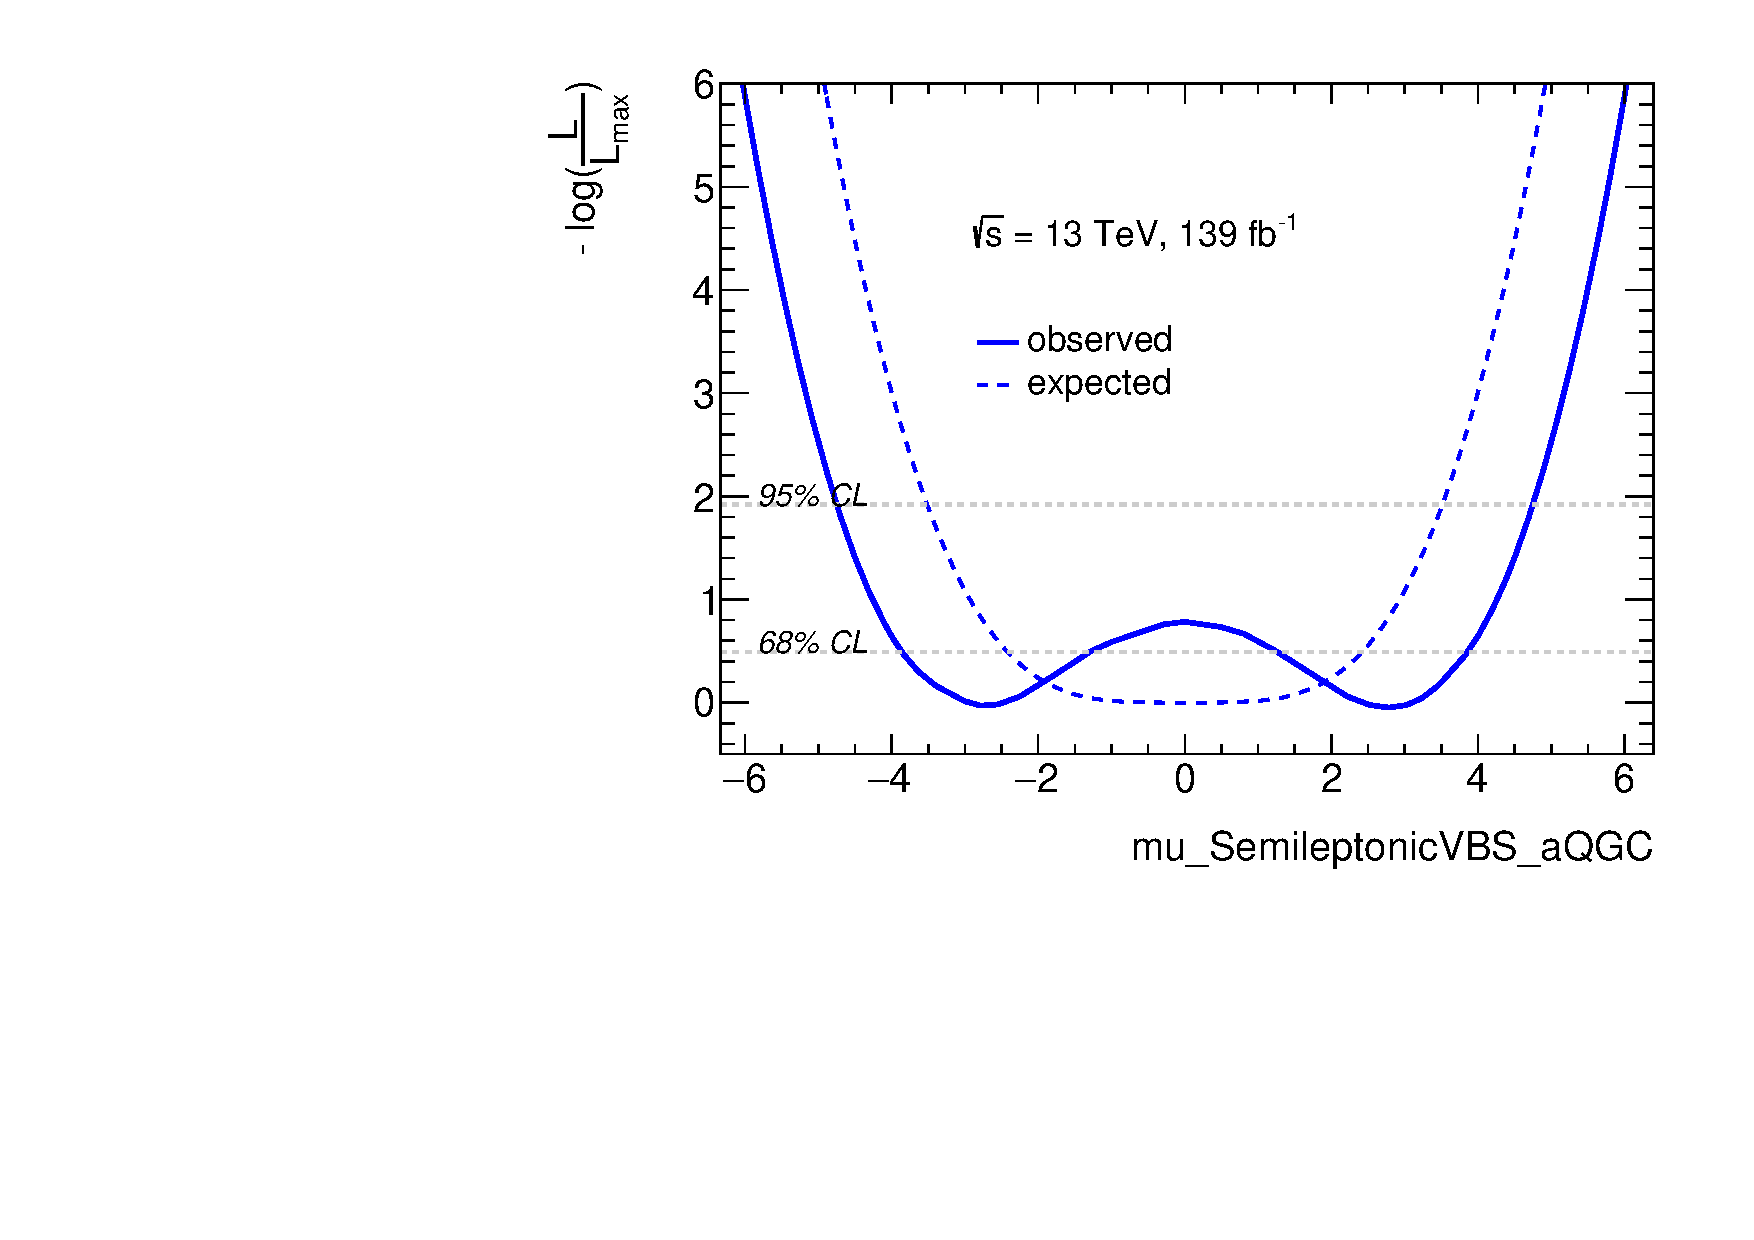
\includegraphics[width=0.38\textwidth]{figures/aQGC/profileFS023000}
        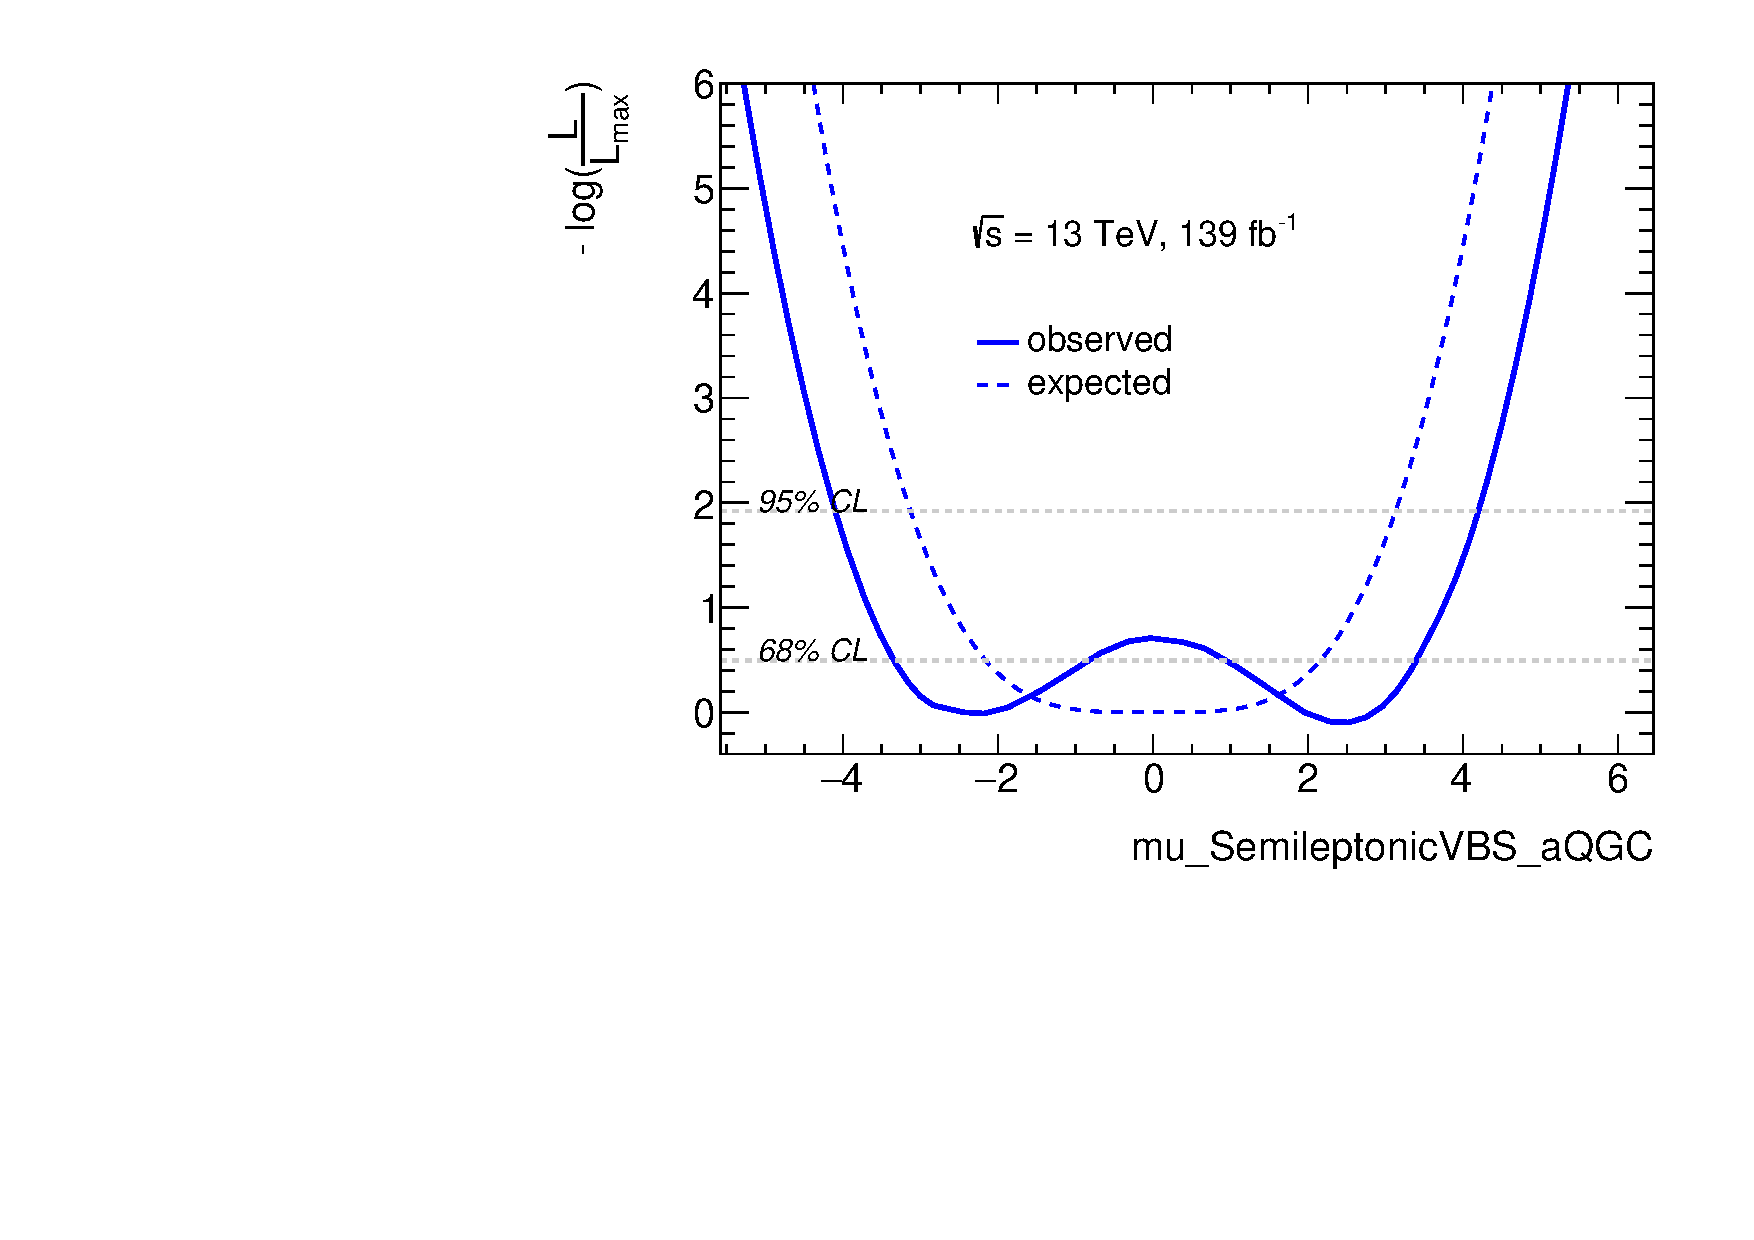
\includegraphics[width=0.32\textwidth]{figures/aQGC/profileFS02inf}
        \caption{The observed log-likelihood curves of FS02 Wilson coefficient where the clipping energy is 1.5~TeV (left), 2.0~TeV (middle), $\infty$ (right).}
        \label{fig:ProfileLLFS}
\end{figure}
\begin{figure}[ht]
    \centering
    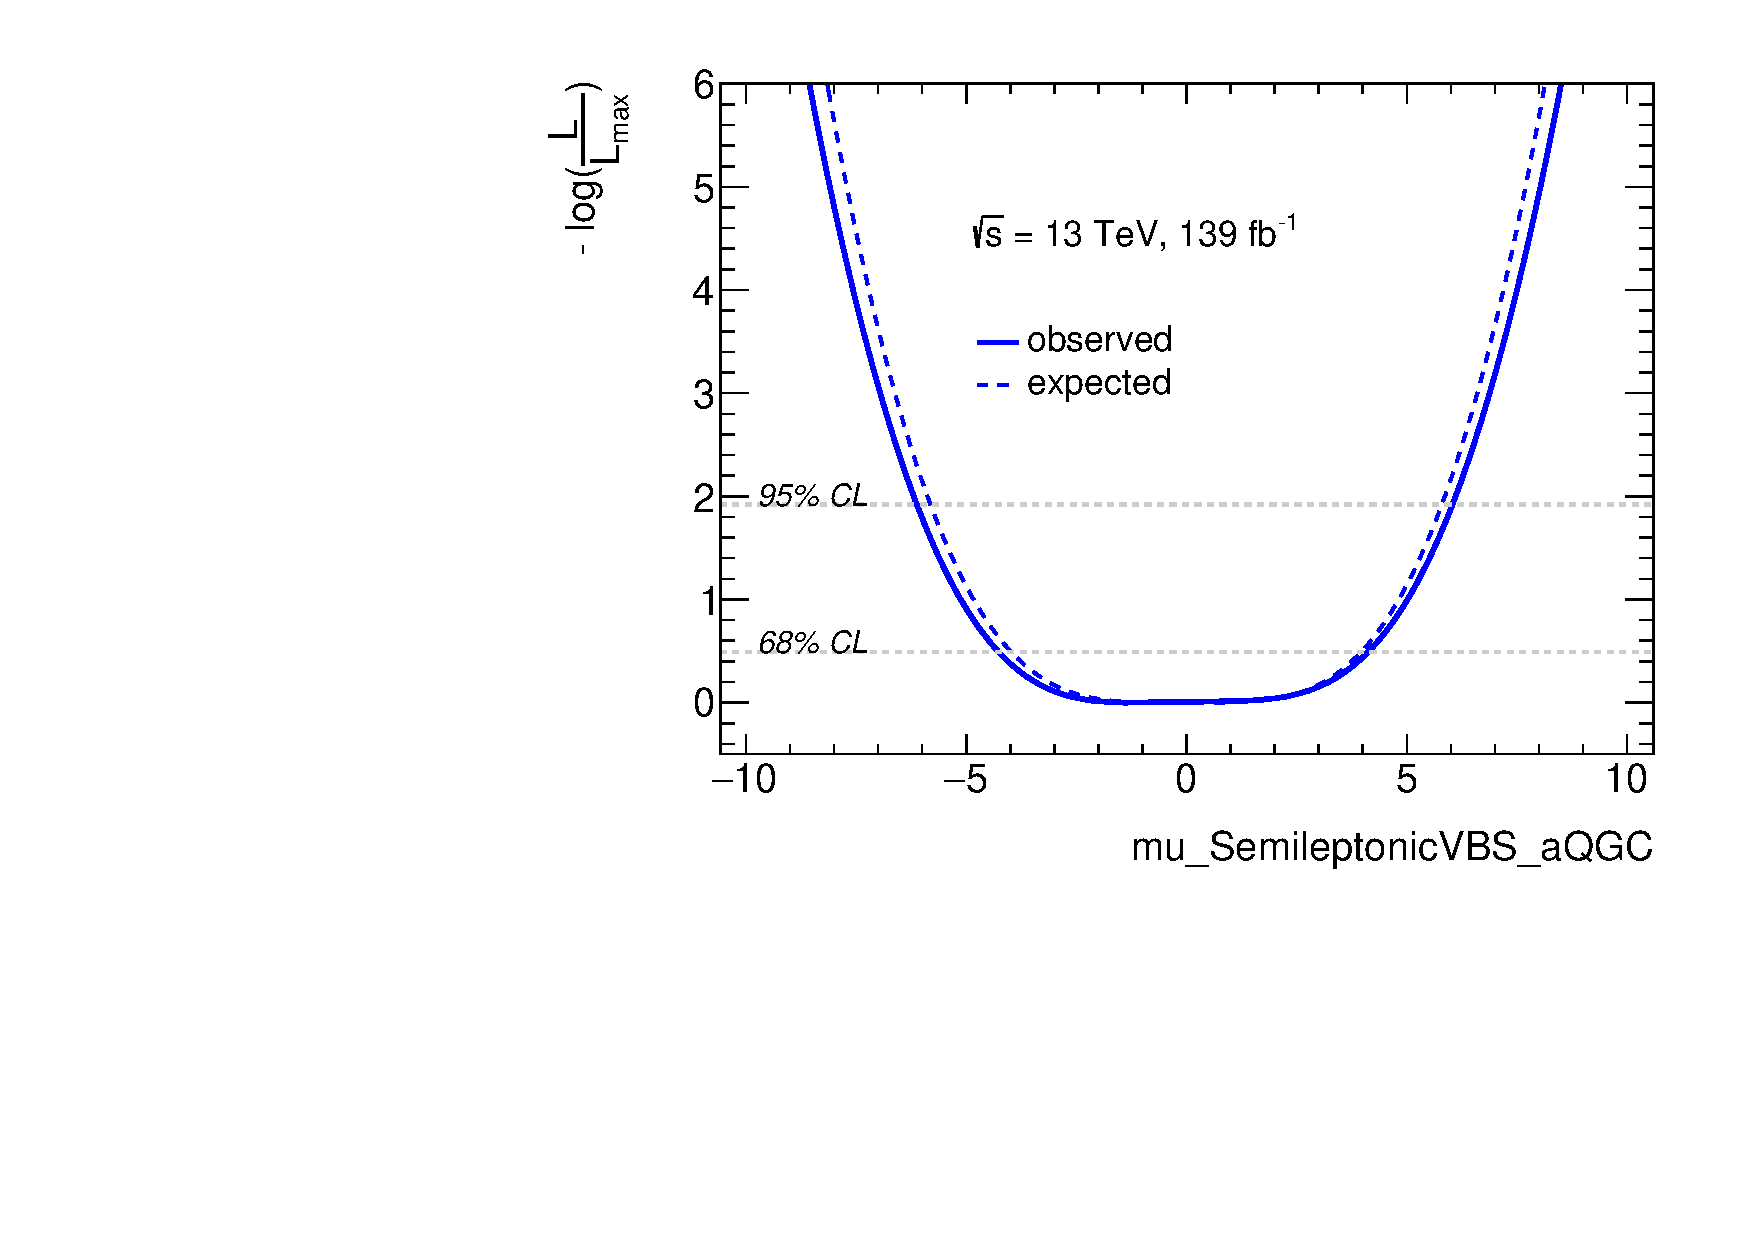
\includegraphics[width=0.32\textwidth]{figures/aQGC/profileFM01500}
    	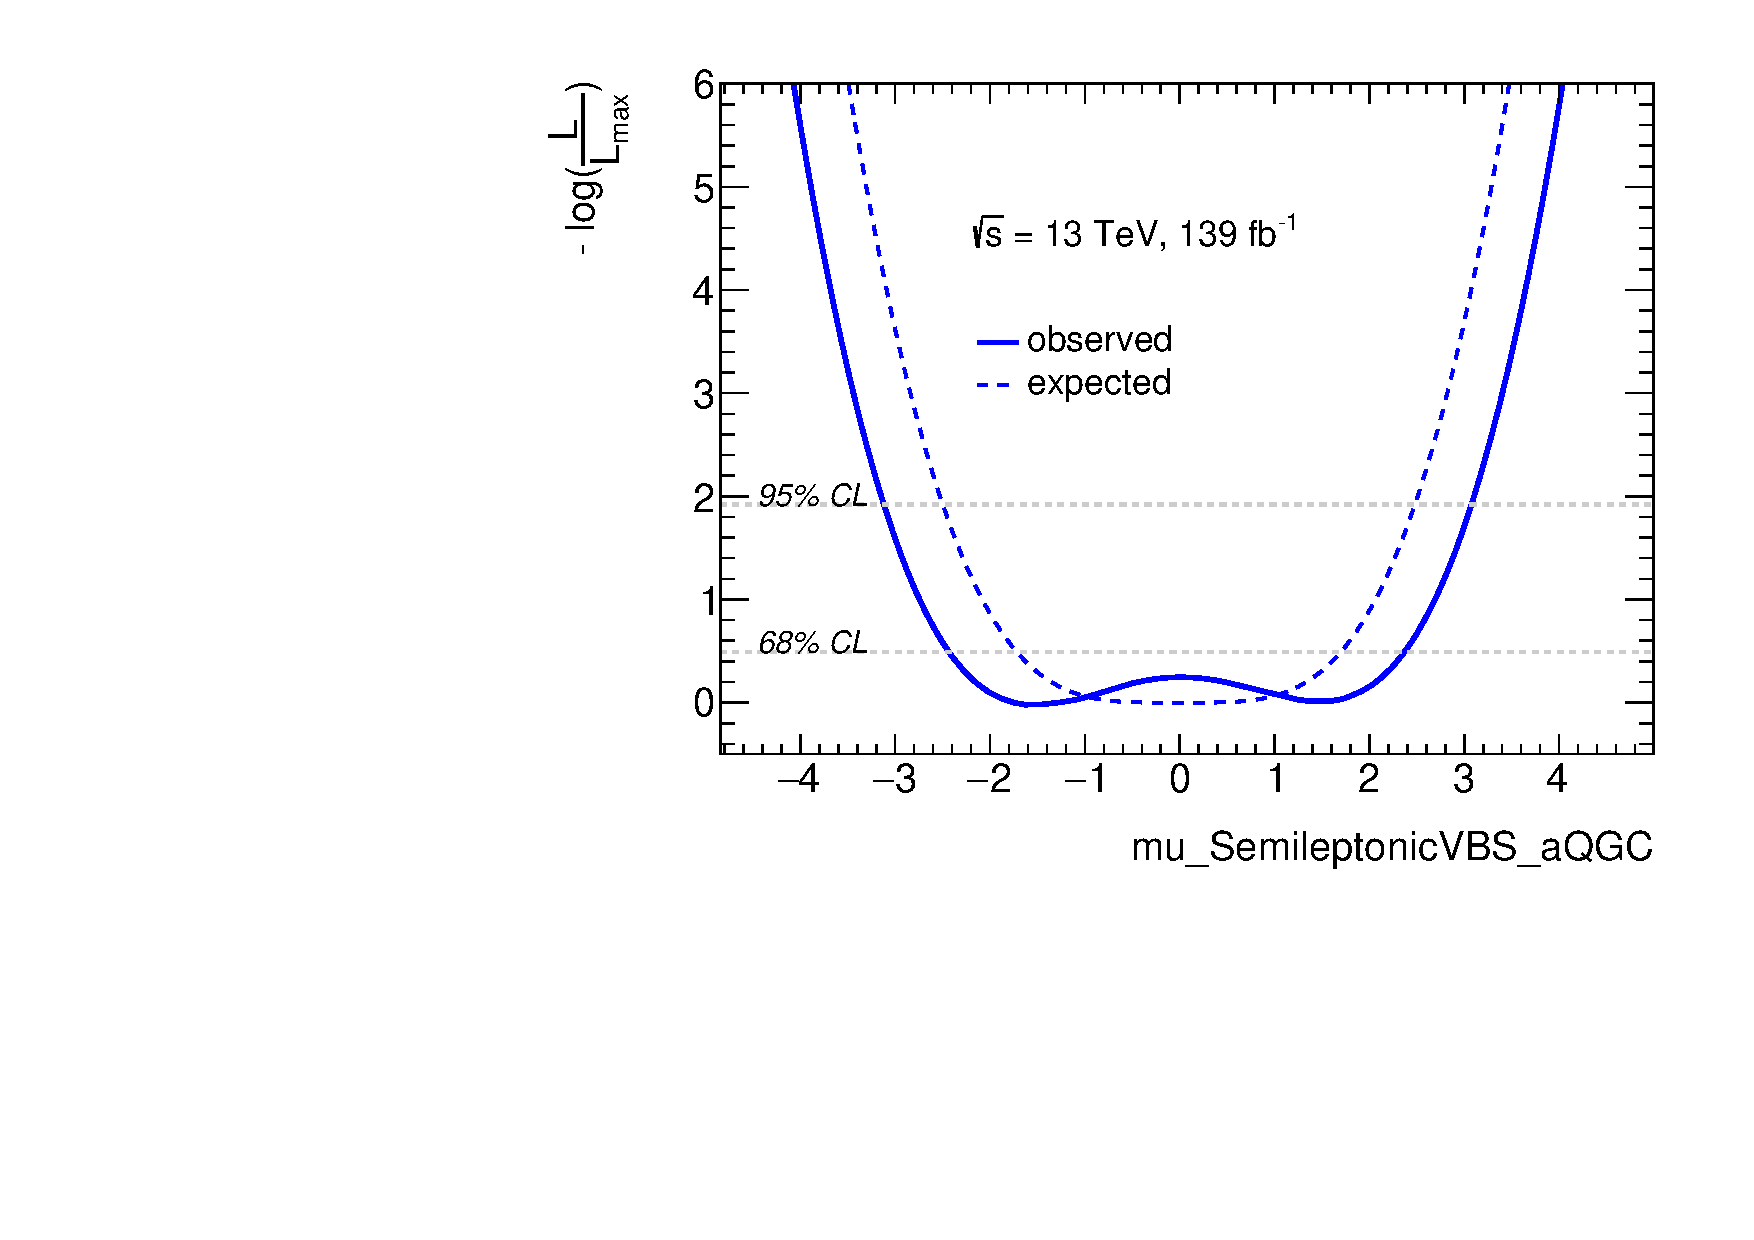
\includegraphics[width=0.32\textwidth]{figures/aQGC/profileFM02000}
    	%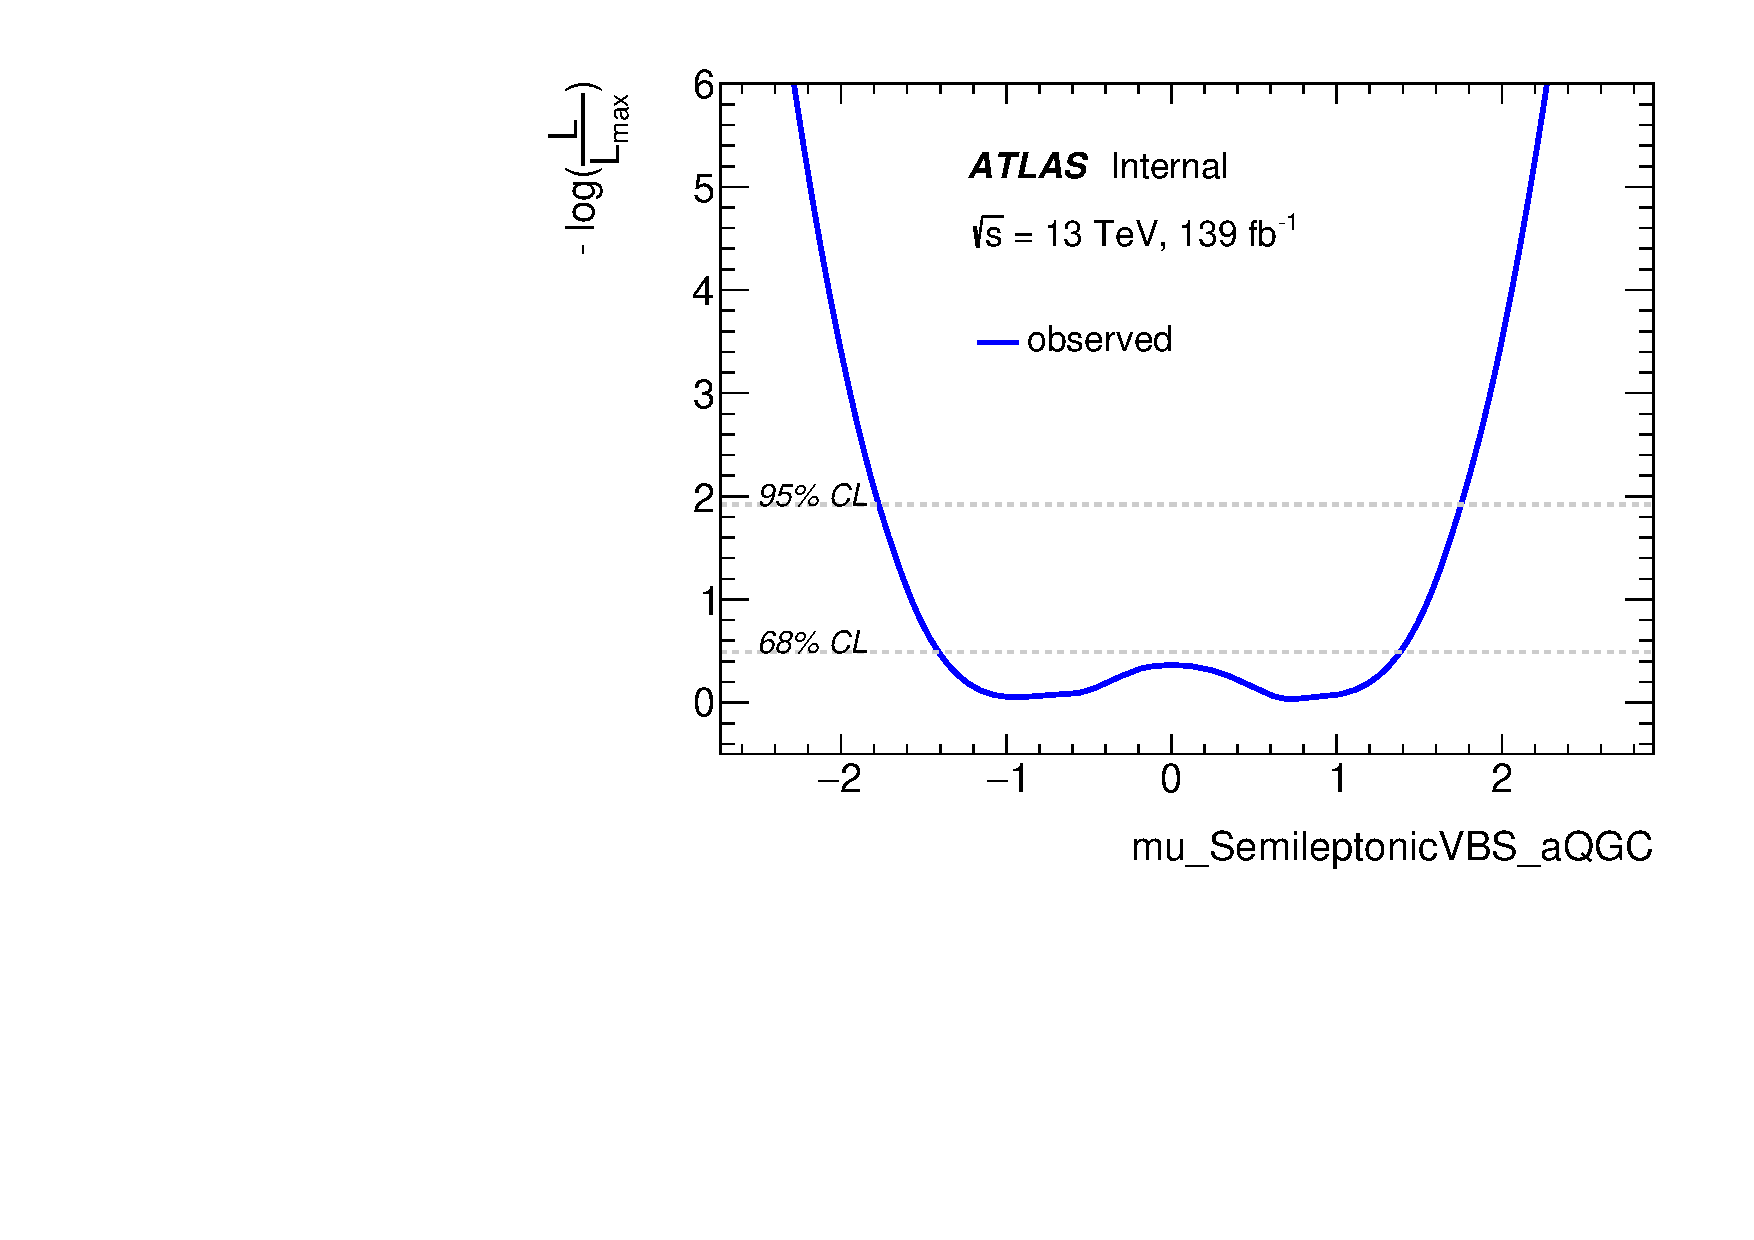
\includegraphics[width=0.38\textwidth]{figures/aQGC/profileFM03000}
        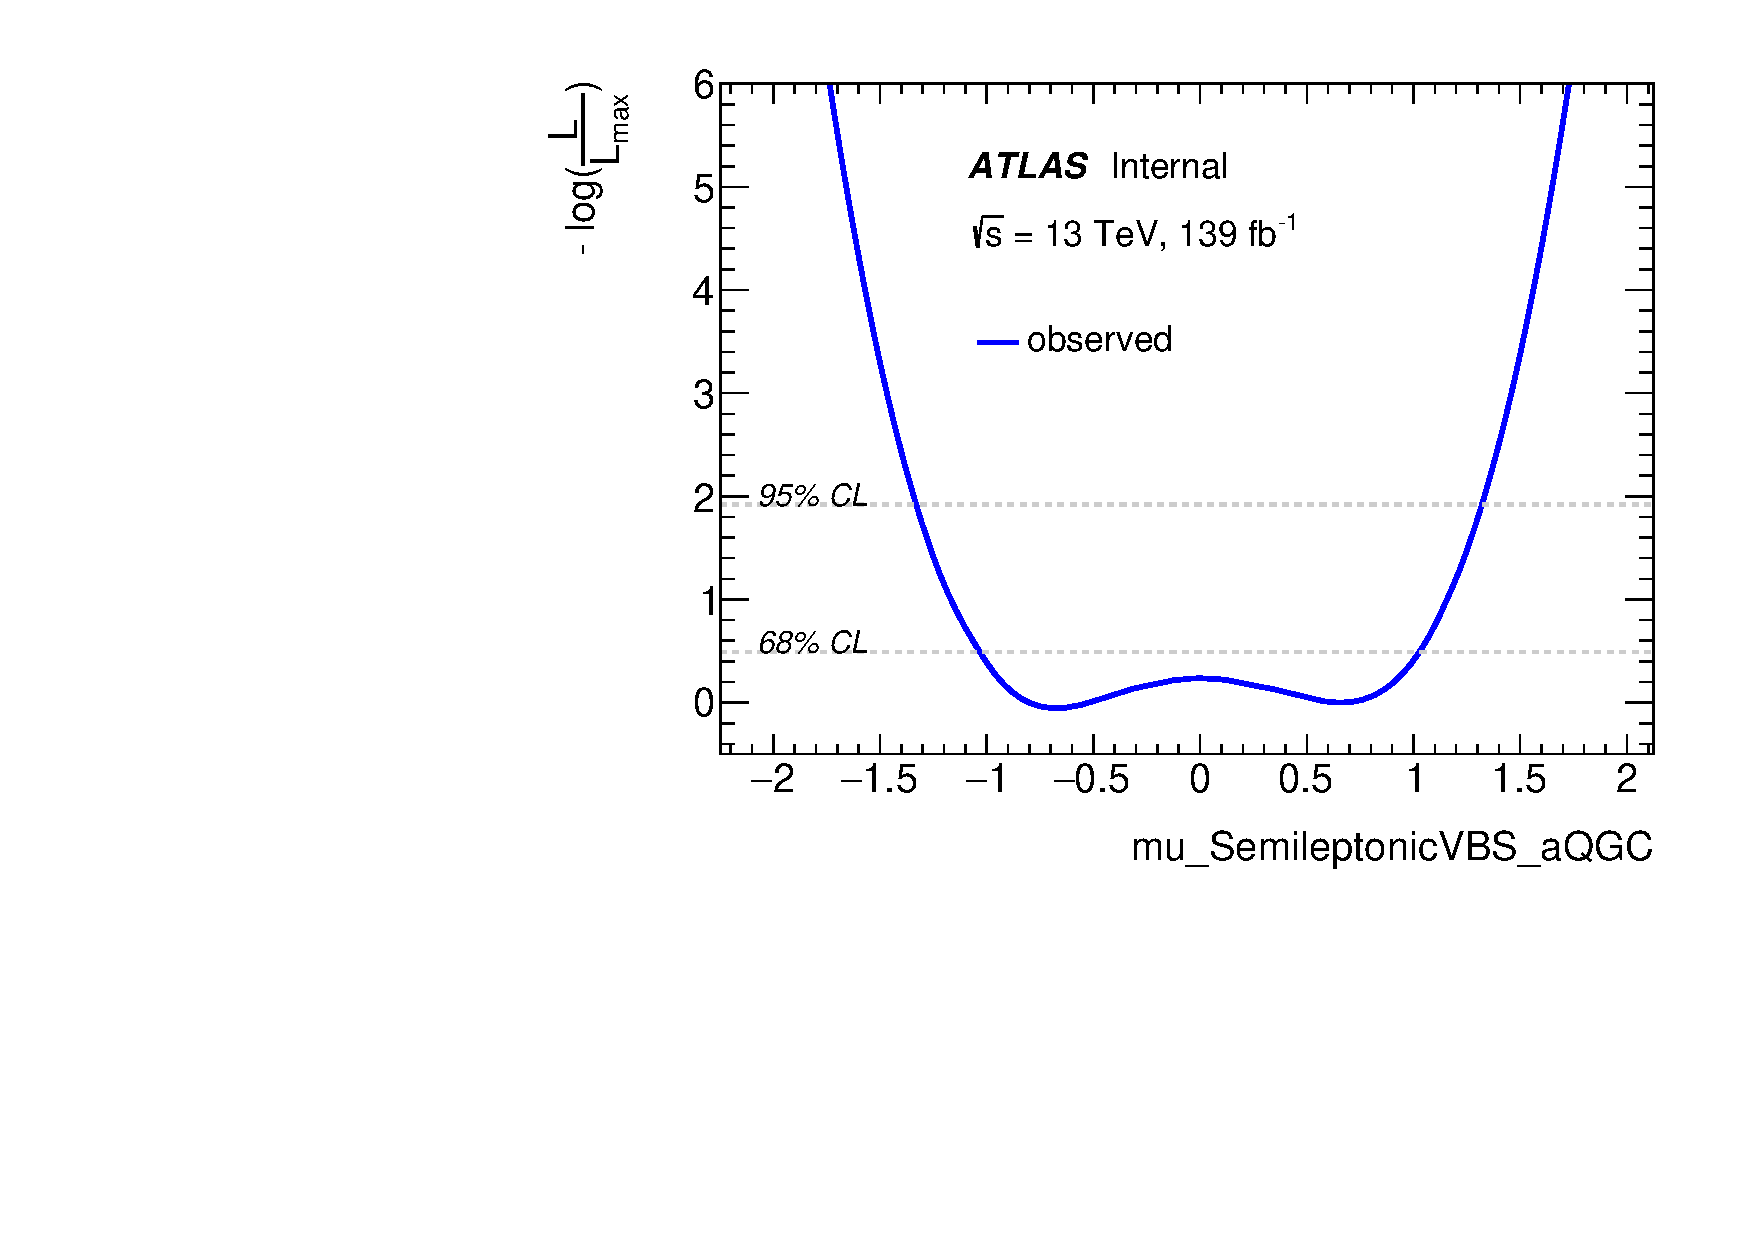
\includegraphics[width=0.32\textwidth]{figures/aQGC/profileFM0inf}
        \caption{The observed log-likelihood curves of FM0 Wilson coefficient where the clipping energy is 1.5~TeV (left), 2.0~TeV (middle), $\infty$ (right).}
        \label{fig:ProfileLLFM}
\end{figure}
%Figure~\ref{fig:QUADINT} shows the distributions of the quardratic term and the interference term for each FT0, FS02, FM0 operator.
%The quardratic term has large contribution compared to the interference term.
Due to the large contribution of the quadratic term in the parametrization of the $\mu_\mathrm{aQGC}$, the log-likelihood curve has two local minimums where there is an excess in data.
At the low clipping value at 1.5~TeV the feature of having the two local minimums gets mild since there is no signal contribution by clipping in the high-mass bins with data excess.
Similar plots for other Wilson coefficients are shown in appendix~\ref{app:aQGCresults}. 
A $\mu_\mathrm{aQGC}$ value at crossing the 95\% confidence interval line and the likelihood curve is used to calculate upper and lower limits on the coefficients. 
%The 95\% confidence interval corresponds to 1.9.
%For high clipping values, the results exclude the signal strength already excluded by the theoretical unitarity bound.
For high clipping values, the observed limit is weaker than the theoretical prediction to conserve the unitarity of the model.
Table~\ref{tab:aQGClimits} shows the uniterized and ununiterized expected and observed limits from figure~\ref{fig:aQGClimits}, where uniterized limit is the intersection point of the theoretical unitality bound and experimental limit line, while ununiterized limit is the limit with no clipping energy.
Distributions of the obtained limit in each clipping value for other Wilson coefficients are shown in appendix~\ref{app:aQGCresults}.
\begin{figure}[ht]
    \centering
    %\includegraphics[width=0.45\textwidth]{figures/aQGC/ClippedFT0CI.pdf}
    %	\includegraphics[width=0.45\textwidth]{figures/aQGC/ClippedFM0CI.pdf}
    %	\includegraphics[width=0.45\textwidth]{figures/aQGC/ClippedFS02CI.pdf}
     \includegraphics[width=0.45\textwidth]{figures/aQGC/FT0limit.pdf}
    	\includegraphics[width=0.45\textwidth]{figures/aQGC/FM0limit.pdf}
    	\includegraphics[width=0.45\textwidth]{figures/aQGC/FS02limit.pdf} 
        \caption{Expected limits (green) and observed limits (blue) for 5 clipping points are shown for each Wilson coefficient FT0 (left), FM0 (right), FS02 (middle). The black line is the theoretical unitarity bound.}
        \label{fig:aQGClimits}
\end{figure}
%\begin{table}[ht!]
%\small
%\begin{center}
%%\resizebox{0.9\textwidth}{!}{
%\begin{tabular}{ | l || l | l | l | l | l |}
%\hline
%                   & 1.5 [ TeV ] & 2.0 [ TeV ] & 3.0 [ TeV ] & 5.0 [ TeV ] & $\infty$                  \tabularnewline \hline
%FT0                & [ -1.02, 0.88 ]  & [ -0.47, 0.41 ]  & [ -0.25, 0.21 ]  & [ -0.16, 0.15 ]  & [ -0.16, 0.16 ]              \tabularnewline \hline
%FM0                & [ -5.63, 5.62 ]  & [ -2.47, 2.47 ]  & [ -1.37, 1.37 ]  & [ -1.08, 1.09 ]  & [ -1.06, 1.07 ]              \tabularnewline \hline

%\caption{Expected limits for each clipping point. Ununiterized limit is shown as the limit with no clipping energy, labeled as $\infty$ in figure~\ref{fig:aQGClimits}.}
%\label{tab:aQGClimits}
%\end{center}
%\end{table}
%uniterized limit
\begin{table}[ht!]
\begin{center}
\resizebox{0.9\textwidth}{!}{
\begin{tabular}{ | l || l | l || l | l | }
\hline
                  &\multicolumn{2}{|l||}{expected limit}                    &\multicolumn{2}{|l|}{observed limit} \tabularnewline \hline
Coefficient&uniterized                            &ununiterized     &uniterized                            &ununiterized \tabularnewline\hline
$f_{T 0} / \Lambda^4$               &[ -0.48, 0.39 ] at [ 1.99, 2.09 ]~TeV &[ -0.16, 0.16 ]  &[ -1.04, 0.74 ] at [ 1.64, 1.78 ]~TeV &[ -0.25, 0.23 ]\tabularnewline\hline
$f_{T 1} / \Lambda^4$              &[ -0.31, 0.31 ] at [ 2.65, 2.63 ]~TeV & [ -0.19, 0.19 ] &[ -0.44, 0.51  ] at [ 2.42, 2.33  ]~TeV &[ -0.25, 0.25 ]\tabularnewline \hline
$f_{T 2} / \Lambda^4$              &[ -0.88, 0.90 ] at [ 2.26, 2.25 ]~TeV & [ -0.41, 0.41 ] &[ -1.35, 1.36 ] at [ 2.04, 2.03 ]~TeV &[ -0.42, 0.52 ]\tabularnewline \hline
$f_{T 5} / \Lambda^4$              &[ -2.87, 2.36 ] at [ 1.50, 1.57 ]~TeV &[ -0.53, 0.51 ]  &[ -3.04, 2.93 ] at [ 1.50, 1.50 ]~TeV & [ -0.46, 0.62 ]\tabularnewline \hline
$f_{T 6} / \Lambda^4$              &[ -2.16, 2.19 ] at [ 1.69, 1.77 ]~TeV  & [ -0.71, 0.68 ]&[ -3.13, 2.87 ] at [ 1.62, 1.66 ]~TeV &[ -0.71, 0.68 ]\tabularnewline \hline
$f_{T 7} / \Lambda^4$             &[ -7.07, 4.05 ] at [ 1.69, 1.91 ]~TeV &[ -1.67, 1.50 ]  &[ -8.39, 6.37 ] at [ 1.62, 1.73 ]~TeV & [ -1.67, 1.50 ]\tabularnewline \hline
$f_{T 8} / \Lambda^4$               &$-$               & [ -0.56, 0.56 ]   &$-$              &[ -0.44, 0.47 ]\tabularnewline \hline
$f_{T 9} / \Lambda^4$              &$-$               & [ -1.16, 1.18 ]   &$-$              &[ -1.02, 0.94 ]\tabularnewline \hline \hline
$f_{S 02} / \Lambda^4$             &[ -5.46, 5.61 ] at [ 2.05, 2.07 ]~TeV &[ -3.27, 3.32 ]  &[ -7.53, 7.80 ] at [ 1.91, 1.90 ]~TeV &[ -3,45, 4.19 ]\tabularnewline\hline
$f_{S 1} / \Lambda^4$              &$-$               & [ -6.70, 6.74 ]   & $-$             &[ -8.57, 8.57 ]\tabularnewline \hline \hline
$f_{M 0} / \Lambda^4$                &[ -3.03, 3.03 ] at [ 1.92, 1.92 ]~TeV &[ -1.06, 1.07 ]  &[ -1.63, 1.63 ] at [ 2.24, 2.24 ]~TeV &[ -1.32, 1.31 ]\tabularnewline \hline
$f_{M 1} / \Lambda^4$                &[ -5.79, 5.80 ] at [ 2.31, 2.31 ]~TeV & [ -3.04, 3.05 ] &[ -8.66, 8.68 ] at [ 2.09, 2.09 ]~TeV &[ -4.01, 4.07 ]\tabularnewline \hline
$f_{M 2} / \Lambda^4$               &$-$               & [ -1.57, 1.57 ]   &$-$              &[ -1.94, 1.94 ]\tabularnewline \hline
$f_{M 3} / \Lambda^4$                &[ -22.11, 21,80 ] at [ 1.59, 1.60 ]~TeV&[ -5.02, 5.01 ]  &[ -22.50, 23.54 ] at [ 1.59, 1.57 ]~TeV &[ -5.93, 6.00 ]\tabularnewline \hline
$f_{M 4} / \Lambda^4$                &[ -4.92, 4.90 ] at [ 2.13, 2.13 ]~TeV & [ -2.36, 2.45 ] &[ -6.27, 6.25 ] at [ 2.0, 2.0 ]~TeV &[ -3.10, 3.10 ]\tabularnewline \hline
$f_{M 5} / \Lambda^4$                &[ -6.39, 6.39 ] at [ 2.37, 2.37 ]~TeV & [ -3.62, 3.62 ] &[ -8.72, 8.74 ] at [ 2.19, 2.19 ]~TeV &[ -4.60, 4.61 ]\tabularnewline \hline
$f_{M 7} / \Lambda^4$                &[ -8.74, 8.41  ] at [ 2.48, 2.50  ]~TeV  & [ -4.99, 4.88 ]   &[ -13.62, 13.13  ] at [ 2.22, 2.24  ]~TeV &[ -6.75, 6.62 ]\tabularnewline \hline
\end{tabular}
}
\caption{Uniterized and ununiterized expected limits and observed limits. Uniterized limit is the intersection point of the theoretical unitality bound and experimental limit line. Ununiterized limit is the limit with no clipping energy, labeled as $\infty$ in figure~\ref{fig:aQGClimits}. Operator FT8, FT9, FS1, FM2 don't have the uniterized limits, since the theoretical unitarity bounds still have more stringent limits.}
\label{tab:aQGClimits}
\end{center}
\end{table}
The ununiterized limits can be compared with the results of other analyses.
Compared to the figure~\ref{fig:limitFT},\ref{fig:limitFM}, \ref{fig:limitFS}, these results give similar or a little weaker limits compared to the CMS results,
which seems due to the difference of the fiducial volume definition.
In the ATLAS experiment limits for the same operators are recently derived in $Z(\nu\bar{\nu})\gamma jj$ channel~\cite{https://doi.org/10.48550/arxiv.2208.12741} with the luminosity of 139~$fb^{-1}$.
The comparison with their results in observed limits is shown in table~\ref{tab:comZnunu}. 
For the tensor type operators $Z(\nu\bar{\nu})\gamma jj$ channel can get more stringent limits because of its fewer backgrounds. 
For the mixed type operators, our channel can get similar or better limits due to its larger production cross section despite the larger backgrounds.
It is desirable to combine the results of several channels in the future since operators which are sensitive are different between each channel.
\begin{table}[ht!]
\begin{center}
\resizebox{0.9\textwidth}{!}{
\begin{tabular}{|c|c|c|}
\hline Coefficient          & Observed limit $\left[\mathrm{TeV}^{-4}\right](Z(\nu\bar{\nu})\gamma jj$) & Observed limit $\left[\mathrm{TeV}^{-4}\right]$ (EW VV+jj semi-lep) \\
\hline$f_{T 0} / \Lambda^4$ & {$[ -9.4, 8.4 ] \times 10^{-2}$}                                    & {$[ -25, 23 ] \times 10^{-2}$} \\
$f_{T 5} / \Lambda^4$       & {$[ -8.8, 9.9 ] \times 10^{-2}$}                                    & {$[ -46, 62 ] \times 10^{-2}$} \\
$f_{T 8} / \Lambda^4$       & {$[ -5.9, 5.9 ] \times 10^{-2}$}                                    & {$[ -44, 47 ] \times 10^{-2}$} \\
$f_{T 9} / \Lambda^4$       & {$[ -1.3, 1.3 ] \times 10^{-1}$}                                    & {$[ -10.2, 9.4 ] \times 10^{-1}$} \\
$f_{M 0} / \Lambda^4$       & {$[ -4.6, 4.6 ]$}                                                   & {$[ -1.3, 1.3 ]$} \\
$f_{M 1} / \Lambda^4$       & {$[ -7.7, 7.7 ]$}                                                   & {$[ -4.0, 4.0 ] $} \\
$f_{M 2} / \Lambda^4$       & {$[ -1.9, 1.9 ]$}                                                   & {$[ -1.9, 1.9 ]$} \\
\hline
\end{tabular}
}
\caption{Comparison of the observed limits derived in $Z(\nu\bar{\nu})\gamma jj$ channel and the EW VV+jj semi-leptonic channel. Uniterization is not preserved.}
\label{tab:comZnunu}
\end{center}
\end{table}
